\def\year{2020}\relax
%File: formatting-instruction.tex
\documentclass[letterpaper]{article} % DO NOT CHANGE THIS
\usepackage{aaai20}  % DO NOT CHANGE THIS
\usepackage{times}  % DO NOT CHANGE THIS
\usepackage{helvet} % DO NOT CHANGE THIS
\usepackage{courier}  % DO NOT CHANGE THIS
\usepackage[hyphens]{url}  % DO NOT CHANGE THIS
\usepackage{graphicx} % DO NOT CHANGE THIS
\usepackage{amssymb}
\usepackage{amsmath}
\usepackage{amstext}
\usepackage{enumerate}
%\usepackage{algorithm}
%\usepackage{algorithmicx}
%\usepackage{algpseudocode}
\usepackage[linesnumbered,boxed]{algorithm2e}
\urlstyle{rm} % DO NOT CHANGE THIS
\def\UrlFont{\rm}  % DO NOT CHANGE THIS
\usepackage{graphicx}  % DO NOT CHANGE THIS
\frenchspacing  % DO NOT CHANGE THIS
\setlength{\pdfpagewidth}{8.5in}  % DO NOT CHANGE THIS
\setlength{\pdfpageheight}{11in}  % DO NOT CHANGE THIS
%\nocopyright
%PDF Info Is REQUIRED.
% For /Author, add all authors within the parentheses, separated by commas. No accents or commands.
% For /Title, add Title in Mixed Case. No accents or commands. Retain the parentheses.
 \pdfinfo{
/Title (Forgetting in CTL to Compute Necessary and Sufficient Conditions)
/Author (Renyan Feng, Erman Acar, Stefan Schlobach, Yisong Wang)
} %Leave this	
% /Title ()
% Put your actual complete title (no codes, scripts, shortcuts, or LaTeX commands) within the parentheses in mixed case
% Leave the space between \Title and the beginning parenthesis alone
% /Author ()
% Put your actual complete list of authors (no codes, scripts, shortcuts, or LaTeX commands) within the parentheses in mixed case.
% Each author should be only by a comma. If the name contains accents, remove them. If there are any LaTeX commands,
% remove them.

% DISALLOWED PACKAGES
% \usepackage{authblk} -- This package is specifically forbidden
% \usepackage{balance} -- This package is specifically forbidden
% \usepackage{caption} -- This package is specifically forbidden
% \usepackage{color (if used in text)
% \usepackage{CJK} -- This package is specifically forbidden
% \usepackage{float} -- This package is specifically forbidden
% \usepackage{flushend} -- This package is specifically forbidden
% \usepackage{fontenc} -- This package is specifically forbidden
% \usepackage{fullpage} -- This package is specifically forbidden
% \usepackage{geometry} -- This package is specifically forbidden
% \usepackage{grffile} -- This package is specifically forbidden
% \usepackage{hyperref} -- This package is specifically forbidden
% \usepackage{navigator} -- This package is specifically forbidden
% (or any other package that embeds links such as navigator or hyperref)
% \indentfirst} -- This package is specifically forbidden
% \layout} -- This package is specifically forbidden
% \multicol} -- This package is specifically forbidden
% \nameref} -- This package is specifically forbidden
% \natbib} -- This package is specifically forbidden -- use the following workaround:
% \usepackage{savetrees} -- This package is specifically forbidden
% \usepackage{setspace} -- This package is specifically forbidden
% \usepackage{stfloats} -- This package is specifically forbidden
% \usepackage{tabu} -- This package is specifically forbidden
% \usepackage{titlesec} -- This package is specifically forbidden
% \usepackage{tocbibind} -- This package is specifically forbidden
% \usepackage{ulem} -- This package is specifically forbidden
% \usepackage{wrapfig} -- This package is specifically forbidden
% DISALLOWED COMMANDS
% \nocopyright -- Your paper will not be published if you use this command
% \addtolength -- This command may not be used
% \balance -- This command may not be used
% \baselinestretch -- Your paper will not be published if you use this command
% \clearpage -- No page breaks of any kind may be used for the final version of your paper
% \columnsep -- This command may not be used
% \newpage -- No page breaks of any kind may be used for the final version of your paper
% \pagebreak -- No page breaks of any kind may be used for the final version of your paperr
% \pagestyle -- This command may not be used
% \tiny -- This is not an acceptable font size.
% \vspace{- -- No negative value may be used in proximity of a caption, figure, table, section, subsection, subsubsection, or reference
% \vskip{- -- No negative value may be used to alter spacing above or below a caption, figure, table, section, subsection, subsubsection, or reference

\setcounter{secnumdepth}{0} %May be changed to 1 or 2 if section numbers are desired.

% The file aaai20.sty is the style file for AAAI Press
% proceedings, working notes, and technical reports.
%
\setlength\titlebox{2.5in} % If your paper contains an overfull \vbox too high warning at the beginning of the document, use this
% command to correct it. You may not alter the value below 2.5 in
\title{Forgetting in CTL to Compute Necessary and Sufficient Conditions }
%Your title must be in mixed case, not sentence case.
% That means all verbs (including short verbs like be, is, using,and go),
% nouns, adverbs, adjectives should be capitalized, including both words in hyphenated terms, while
% articles, conjunctions, and prepositions are lower case unless they
% directly follow a colon or long dash
\author{Written by AAAI Press Staff\textsuperscript{\rm 1}\thanks{Primarily Mike Hamilton of the Live Oak Press, LLC, with help from the AAAI Publications Committee}\\ \Large \textbf{AAAI Style Contributions by
Pater Patel Schneider,} \\ \Large \textbf{Sunil Issar, J. Scott Penberthy, George Ferguson, Hans Guesgen}\\ % All authors must be in the same font size and format. Use \Large and \textbf to achieve this result when breaking a line
\textsuperscript{\rm 1}Association for the Advancement of Artificial Intelligence\\ %If you have multiple authors and multiple affiliations
% use superscripts in text and roman font to identify them. For example, Sunil Issar,\textsuperscript{\rm 2} J. Scott Penberthy\textsuperscript{\rm 3} George Ferguson,\textsuperscript{\rm 4} Hans Guesgen\textsuperscript{\rm 5}. Note that the comma should be placed BEFORE the superscript for optimum readability
2275 East Bayshore Road, Suite 160\\
Palo Alto, California 94303\\
publications20@aaai.org % email address must be in roman text type, not monospace or sans serif
}
 \begin{document}

\newcommand{\tuple}[1]{{\langle{#1}\rangle}}
\newcommand{\Mod}{\textit{Mod}}
\newcommand\ie{{\it i.e. }}
\newcommand\eg{{\it e.g.}}
\newcommand\st{{\it s.t. }}
\newtheorem{definition}{Definition}
\newtheorem{examp}{Example}
\newenvironment{example}{\begin{examp}\rm}{\end{examp}}
\newtheorem{lemma}{Lemma}
\newtheorem{proposition}{Proposition}
\newtheorem{theorem}{Theorem}
\newtheorem{corollary}[theorem]{Corollary}
\newenvironment{proof}{{\bf Proof:}}{\hfill\rule{2mm}{2mm}\\ }
\newcommand{\rto}{\rightarrow}
\newcommand{\lto}{\leftarrow}
\newcommand{\lrto}{\leftrightarrow}
\newcommand{\Rto}{\Rightarrow}
\newcommand{\Lto}{\Leftarrow}
\newcommand{\LRto}{\Leftrightarrow}
\newcommand{\Var}{\textit{Var}}
\newcommand{\Forget}{\textit{Forget}}
\newcommand{\KForget}{\textit{KForget}}
\newcommand{\TForget}{\textit{TForget}}
%\newcommand{\forget}{\textit{forget}}
\newcommand{\Fst}{\textit{Fst}}
\newcommand{\dep}{\textit{dep}}
\newcommand{\term}{\textit{term}}
\newcommand{\literal}{\textit{literal}}

\newcommand{\Atom}{\mathcal{A}}
\newcommand{\SFive}{\textbf{S5}}
\newcommand{\MPK}{\textsc{k}}
\newcommand{\MPB}{\textsc{b}}
\newcommand{\MPT}{\textsc{t}}
\newcommand{\MPA}{\forall}
\newcommand{\MPE}{\exists}

\newcommand{\DNF}{\textit{DNF}}
\newcommand{\CNF}{\textit{CNF}}

\newcommand{\degree}{\textit{degree}}
\newcommand{\sunfold}{\textit{sunfold}}

\newcommand{\Pos}{\textit{Pos}}
\newcommand{\Neg}{\textit{Neg}}
\newcommand\wrt{{\it w.r.t.}}
\newcommand{\Hm} {{\cal M}}
\newcommand{\Hw} {{\cal W}}
\newcommand{\Hr} {{\cal R}}
\newcommand{\Hb} {{\cal B}}
\newcommand{\Ha} {{\cal A}}

\newcommand{\Dsj}{\triangledown}

\newcommand{\wnext}{\widetilde{\bigcirc}}
\newcommand{\nex}{\bigcirc}
\newcommand{\ness}{\square}
\newcommand{\qness}{\boxminus}
\newcommand{\wqnext}{\widetilde{\circleddash}}
\newcommand{\qnext}{\circleddash}
\newcommand{\may}{\lozenge}
\newcommand{\qmay}{\blacklozenge}
\newcommand{\unt} {{\cal U}}
\newcommand{\since} {{\cal S}}
\newcommand{\SNF} {\textit{SNF$_C$}}
\newcommand{\start}{\textbf{start}}
\newcommand{\Elm}{\textit{Elm}}
\newcommand{\simp}{\textbf{simp}}
\newcommand{\nnf}{\textbf{nnf}}

\newcommand{\CTL}{\textrm{CTL}}
\newcommand{\Ind}{\textrm{Ind}}
\newcommand{\Tran}{\textrm{Tran}}
\newcommand{\Sub}{\textrm{Sub}}
\newcommand{\NI}{\textrm{NI}}
\newcommand{\Inst}{\textrm{Inst}}
\newcommand{\Com}{\textrm{Com}}
\newcommand{\Rp}{\textrm{Rp}}
\newcommand{\forget}{{\textsc{f}_\CTL}}
\newcommand{\ALL}{\textsc{a}}
\newcommand{\EXIST}{\textsc{e}}
\newcommand{\NEXT}{\textsc{x}}
\newcommand{\FUTURE}{\textsc{f}}
\newcommand{\UNTIL}{\textsc{u}}
\newcommand{\GLOBAL}{\textsc{g}}
\newcommand{\UNLESS}{\textsc{w}}
\newcommand{\Def}{\textrm{def}}
\newcommand{\IR}{\textrm{IR}}
\newcommand{\Tr}{\textrm{Tr}}
\newcommand{\dis}{\textrm{dis}}
\def\PP{\ensuremath{\textbf{PP}}}
\def\NgP{\ensuremath{\textbf{NP}}}
\def\W{\ensuremath{\textbf{W}}}
\newcommand{\Pre}{\textrm{Pre}}
\newcommand{\Post}{\textrm{Post}}


\newcommand{\CTLsnf}{{\textsc{SNF}_{\textsc{ctl}}^g}}
\newcommand{\ResC}{{\textsc{R}_{\textsc{ctl}}^{\succ, S}}}
\newcommand{\CTLforget}{{\textsc{F}_{\textsc{ctl}}}}
\newcommand{\Refine}{\textsc{Refine}}
\newcommand{\cf}{\textrm{cf.}}
\newcommand{\NEXP}{\textmd{\rm NEXP}}
\newcommand{\EXP}{\textmd{\rm EXP}}
\newcommand{\coNEXP}{\textmd{\rm co-NEXP}}
\newcommand{\NP}{\textmd{\rm NP}}
\newcommand{\coNP}{\textmd{\rm co-NP}}
\newcommand{\Pol}{\textmd{\rm P}}
\newcommand{\BH}[1]{\textmd{\rm BH}_{#1}}
\newcommand{\coBH}[1]{\textmd{\rm co-BH}_{#1}}
\newcommand{\Empty}{\varnothing}
\newcommand{\NLOG}{\textmd{\rm NLOG}}
\newcommand{\DeltaP}[1]{\Delta_{#1}^{p}}
\newcommand{\PIP}[1]{\Pi_{#1}^{p}}
\newcommand{\SigmaP}[1]{\Sigma_{#1}^{p}}



\maketitle

\begin{abstract}
Computation Tree Logic (CTL) is one of the central formalisms in formal verification. As a specification language, it is used to express a property
that the system at hand is expected to satisfy. From
both the verification and the system design points
of view, some information content of such property might become irrelevant for the system due to
various reasons e.g., it might become obsolete by
time, or perhaps infeasible due to practical difficulties. Then, the problem arises on how to subtract such piece of information without altering the
relevant system behaviour or violating the existing
specifications. Moreover, in such a scenario, two
crucial notions are informative: the strongest necessary condition (SNC) and the weakest sufficient
condition (WSC) of a given property.


To address such a scenario in a principled way, we
introduce a forgetting-based approach in CTL and
show that it can be used to compute SNC and WSC
of a property under a given model. We study its
theoretical properties and also show that our notion
of forgetting satisfies existing essential postulates.
Furthermore, we analyse the computational complexity of basic tasks, including various results for
the relevant fragment $\CTL_{\ALL\FUTURE}$.
\end{abstract}

\section{Introduction}
Consider a car-manufacturing company which produces two types of automobiles: a sedan car (basically a four-doored classical passenger car) and a sports car.  No matter a sedan or a sports car, both production lines are subject to a single standard criterion which is indispensable: safety restrictions.  This shared feature is also complemented several major differences aligned with these types in general. That is, a sedan car is produced with a small engine, while a sports car is produced with a large one. Moreover, due to its large amount of production, the sedan car is subject to some very restrictive low-carbon emission regulations, while a sports car is not. On the verge of shifting to an upcoming new engine technology, the company aims to adapt the sedan production to electrical engines. Such major shift in production also comes with one in regulations; electric sedans are not subject to low-carbon emission restrictions any more. In fact, due to the difference in its underlying technology, a sedan car drastically emits much less carbon, hence such standard is obsolete, and can be dropped. Yet dropping some restrictions in a large and complex production system in automative industry, without affecting the working system components or violating dependent specifications  is a non-trivial task.


Similar scenarios may arise in many different domains such as business-process modelling, software development, concurrent systems and more~\cite{Baier:PMC:2008}.  In general,  some information content of such property might become irrelevant for the system due to various reasons e.g., it might become obsolete by time like in the above example, or perhaps  becomes infeasible due to practical difficulties. Then, the problem arises on how to subtract such piece of information without altering the behaviour of the relevant system components or violating the existing specifications. Moreover, in such a scenario, two logical notions introduced by E. Dijkstra in~\cite{dijkstra1978guarded} are very informative: the \emph{strongest necessary condition} (SNC) and the \emph{weakest sufficient condition}  (WSC)  of a given specification. These correspond to \emph{most general consequence} and the \emph{most specific abduction} of such specification, respectively.

%\emph{Weakest precondition}, we also call \emph{weakest sufficient condition} (WSC)
%\emph{Strongest postcondition} (we also call \emph{strongest necessary condition} (SNC)), a dual concept, was introduced subsequently.





To address such a scenario in a principled way, we employ a  method based on formal verification.\footnote{ This is  especially useful for abstracting away the domain-dependent problems, and focusing on conceptual ones.} In particular,
we introduce a \emph{forgetting}-based approach in Computation Tree Logic (\CTL)~\cite{clarke1981design}
a central formalism in formal verification, and show that it can
be used to compute SNC and WSC, in the same spirit of~\cite{DBLP:journals/ai/Lin01}.
%\begin{example}\label{exmp:1}


The scenario we mentioned concerning car-engine manufacturing can be easily represented  as a small example by the following Kripke structure $\Hm=(S, R, L, s_0)$ in Figure~\ref{BVM} on $V=\{ sl, sr, se, le, lc\}$ whose elements correspond to  \emph{select},  \emph{safety restrictions}, \emph{small engine},  \emph{large engine} and \emph{low-carbon emission requirements}, respectively. Moreover, $s_0$ is the initial state where we select either choose producing an engine for \emph{sedan} which corresponds to the state $s_1$ or a \emph{sports car} which corresponds to the state $s_2$.
Since only a single-type of production is possible at a time, after each production state ($s_1$ or $s_2$), we turn back to the initial state ($s_0$) to start over.
%Let $\varphi=\ALL\GLOBAL \ALL \FUTURE(sr)$, which means $sr$ will be satisfied infinitely many times in the structure, be a \CTL\ formula.
\begin{figure}[ht]
  \centering
  % Requires \usepackage{graphicx}
  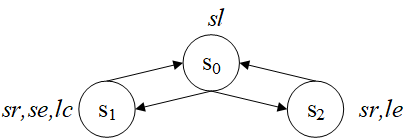
\includegraphics[width=5cm]{BVM.png}\\
  \caption{Car Engine Manufacturing Scenario }\label{BVM}
\end{figure}
%\end{example}






%In program correctness methods, SNC and WSC meet their toughest challenge when
%they deal with iterative constructs~\cite{mraihi2011computing}.
%{\em Computation Tree Logic} (\CTL)~\cite{clarke1981design}


%Model modification, which has been developed in~\cite{ramdani2019r,martinez2016ctl,ding2006ctl}, is an extension of refinement of system.
%This paper explore a method to compute the WSC of a property (a \CTL\ formula) under a given model system that may be modified for guiding \CTL\ Model modification.
%It is known that the computing of WSC for code fragment $S$ with respect to assertion $Q$  requires $S$  must terminate~\cite{tremblay1996logic}.
%test
%It is known that the computing of WSC for code fragment $S$ with respect to assertion $Q$  requires $S$  must terminate~\cite{tremblay1996logic} since to it just concerns relation among input values and output values.
%However, in the case of model checking, it concerns properties about execution runs, which may not terminate.
%For example, the concurrent system with there is at least one successor state for each state $s$ in this system, the termination of this system is impossible.
%However, in \emph{model checking} of concurrent system with there is at least one successor state for each state $s$ in this system, the termination of this system is impossible.
%Informally, given a transition system $\Hm$ with $s_0$ as an initial state and a specification $\varphi$ (in this article we suppose it is a {\em Computation Tree Logic}
%(\CTL\ in short)~\cite{clarke1981design} formula), we should decide whether $(\Hm, s_0) \models \varphi$. It is a good thing if $(\Hm, s_0) \models \varphi$ indeed. However, if $(\Hm, s_0) \nvDash \varphi$, how can we find the WSC $\psi$ under a given set of atoms such that $(\Hm, s_0) \models \psi \supset \varphi$.
%It can be shown by the following example.


The notions of SNC and WSC were considered in the scope of formal verification among others,  in generating counterexamples~\cite{dailler2018instrumenting} and refinement of  system~\cite{woodcock1990refinement}.
On the \emph{forgetting} side, it was first formally defined
in propositional and first order logics by Lin and Reiter~\cite{lin1994forget}.
Over the last decades, researchers have developed forgetting notions and theories not only in classical logic but also in non-classical logic systems~\cite{eiter2019brief}, such as forgetting in logic programs under answer-set semantics~\cite{DBLP:Zhang:AIJ2006,Eiter2008Semantic,Wong:PhD:Thesis,Yisong:KR:2012,Yisong:IJCAI:2013}, description logics~\cite{Wang:AMAI:2010,Lutz:IJCAI:2011,zhao2017role} and knowledge forgetting in modal logic~\cite{Yan:AIJ:2009,Kaile:JAIR:2009,Yongmei:IJCAI:2011,fang2019forgetting}. It also has been considered in planning~\cite{lin2003compiling} and conflict solving \cite{Lang2010Reasoning,Zhang2005Solving},
%knowledge compilation \cite{Zhang2009Knowledge,Bienvenu2010Knowledge},
creating restricted views of ontologies~\cite{zhao2017role},
%{ZhaoSchmidt18a},
strongest and weakest definitions \cite{Lang2008On}, SNC (WSC) \cite{DBLP:journals/ai/Lin01}, among others.

%\begin{example}\label{exmp:1}
% We give a simplified variant of an example from~\cite{Baier:PMC:2008}. A Beverage Vending Machine %, which has been established as standard in the field of process calculi,
% can be described as a Kripke structure $\Hm=(S, R, L, s_0)$ in Figure~\ref{BVM} on $V_a=\{select, pay, beer, soda\}$.
% % with $S=\{s_0, s_1, s_2\}$, $R=\{(s_0, s_1), (s_0, s_2), (s_1, s_0), (s_2,s_0)\}$, $L(s_0)=\{select\}$, $L(s_1)=\{pay, soda\}$, $L(s_2)=\{pay, beer\}$ and $s_0$ is an initial state.
%This means that  if we are in $s_0$, (s)elect (so)da and pay for it then we are in $s_1$, else if we (s)elect (b)eer and (p)ay for it then we  are in $s_2$, after taking out the drink we are back to $s_0$ again.
%For convenience, we use $s$ for $select$, $p$ for $pay$, $b$ for $beer$, $so$ for $soda$ and $r$ for orange juice.
%%It follows that $s_0$ is an initial state.
%Let $\varphi=\ALL\GLOBAL \ALL \FUTURE(p\wedge r)$, which means $p\wedge r$ will be satisfied infinite times in the structure, be a \CTL\ formula.
%\begin{figure}
%  \centering
%  % Requires \usepackage{graphicx}
%  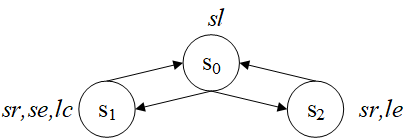
\includegraphics[width=5cm]{BVM.png}\\
%  \caption{A Beverage Vending Machine}\label{BVM}
%\end{figure}
%\end{example}
Although forgetting has been extensively investigated from various aspects of different logical systems, the existing forgetting techniques are not directly applicable in \CTL.
For instance, in propositional forgetting theory, forgetting atom $q$ from $\varphi$ is equivalent to a formula $\varphi[q/\top] \vee \varphi[q/\perp]$, where $\varphi[q/X]$ is a formula obtained from $\varphi$ by replacing each $q$ with $X$ ($X\in \{\top, \perp\}$).
This method cannot be extended to a \CTL\ formula. Consider a \CTL\ formula $\psi=\ALL\GLOBAL p \wedge \neg \ALL\GLOBAL q \wedge \neg \ALL\GLOBAL \neg q$. If we want to forget
atom $q$ from $\psi$ by using the above method, we would have $\psi[q/\top] \vee \psi[q/\perp] \equiv \perp$. This is obviously not correct since after forgetting $q$ this specification should
not become inconsistent.
Similar to~\cite{Yan:AIJ:2009}, we research forgetting in \CTL\ from the semantic forgetting point of view.
And it is shown that our definition of forgetting satisfies those four postulates of forgetting presented in~\cite{Yan:AIJ:2009}.
%We can decide $(\Hm, s_0)\nvDash \varphi$ easily since this structure does not contain the atom $r$.
%In order for $(\Hm, s_0)$ to satisfy $\varphi$, we should find a condition $\psi$ such that $(\Hm, s_0) \models \psi \supset \varphi$.
% As we know that if this condition exists, there are also many other conditions that satisfy the need.
%In this is the case, we can analyze in advance the set of possible atomic propositions that make up the condition. Then we can find this condition in the set only. And the smaller the set, the easier to find out the condition.
%In this paper, we always assume that the condition is a property defined on the specified atomic proposition set $V$, for our example $V=\{p,r\}$, and find the weakest property (that is, the weakest sufficient condition) satisfying the condition on the set. Finding this property is called discovering theorem by Lin in~\cite{DBLP:journals/aim/Lin18}.

%However, since $\Hm$ is a Kripke structure, it needs to be converted into a logical formula (theory), that is the characterizing formula, which is in \CTL\  proposed in~\cite{DBLP:journals/tcs/BrowneCG88}.
%We find the WSC in a set $V$ of atoms, hence a set-based bisimulation between two \MPK-structures (a Kripke structure with a state in it), $V$-bisimulation, and characterizing formula on $V$ will be proposed in this paper.
%Although the relation of bisimulation between transition systems has been wildly researched during the past several decades, it is different from our concept.
%Our $V$-bisimulation is a more general bisimulation than others.
%On the one hand, the above set-based bisimulation is an extension of the
%bisimulation-equivalence of Definition~7.1 in \cite{Baier:PMC:2008} in the
%sense that, if $V=\cal A$, then our bisimulation is almost same to the
%latter.
%\footnote{The latter has a given set of initial states,
%while there is only one initial state in our case.}.
%On the other hand, the above set-based bisimulation notion is similar to
%the state equivalence in \cite{DBLP:journals/tcs/BrowneCG88}. But it is
%different in the sense that ours is defined on \MPK-structures,
%while it is defined on states in \cite{DBLP:journals/tcs/BrowneCG88}.
%Moreover, the set-based bisimulation notion is also different
%from  the state-based bisimulation notion of Definition~7.7 in \cite{Baier:PMC:2008},
%which is defined for states of a given \MPK-structure.
The rest of the paper is organised as follows. Section 2 introduces the notation and technical preliminaries. As key contributions, Section 3, introduces the notion of forgetting in \CTL, via developing the notion of $V$-bisimulation. Such bisimulation is constructed through a set-based bisimulation and more general than the classical bisimulation. Moreover,  it provides a CTL characterization for model structures (with the initial state), and studies the semantic properties of forgetting. In addition, a complexity analysis, including a relevant fragment  $\CTL_{\ALL\FUTURE}$, is carried out.
Section 4 explores the relation between forgetting and SNC (WSC). Section 5 gives a model-based algorithm for computing forgetting in \CTL\ and outline its complexity. Conclusion closes the paper.


Due to space restrictions and to avoid hindering the flow of content, all the proofs are put to the supplementary material.



\section{Preliminaries}
 We start with some technical and notational preliminaries. Throughout this paper, we fix a finite set $\Ha$ of propositional variables (or atoms), and use $V$, $V'$ for subsets of $\Ha$.
\subsection{Model structure in $\CTL$}
In general, a transition system
%\footnote{According to \cite{Baier:PMC:2008},
%a {\em transition system} TS is a tuple $(S, Act,\rto,I, AP, L)$ where
%(1) $S$ is a set of states,
%(2) $\textrm{Act}$ is a set of actions,
%(3) $\rto\subseteq S\times \textrm{Act}\times S$ is a transition relation,
%(4) $I\subseteq S$ is a set of initial states,
%(5) $\textrm{AP}$ is a set of atomic propositions, and
%(6) $L:S\rto 2^{\textrm{AP}}$ is a labeling function.}
 can be described by a \emph{model\ structure} (or \emph{Kripke \ structure}) (see~\cite{Baier:PMC:2008} for details). A model structure is a triple $\Hm=(S,R,L)$, where
\begin{itemize}
  \item $S$ is a finite nonempty set of states \footnote{Indeed, every state is identified by a configuration of atoms i.e., which holds in that state.},
  \item $R\subseteq S\times S$ and, for each $s\in S$, there
  is $s'\in S$ such that $(s,s')\in R$,
  \item $L$ is a labeling function $S\rto 2^{\cal A}$.
\end{itemize}
%We call a model structure $\Hm$ on a set $V$ of atoms if $L: S \rto 2^V$, i.e., the labelling function $L$ map every state to $V$ (not the $\Ha$).
Given a model structure $\Hm=(S,R,L)$, a \emph{path} $\pi_{s_i}$ starting from $s_i$ of $\Hm$ is an infinite sequence of states $\pi_{s_i}=(s_i, s_{i+1} s_{i+2},\dots)$, where for each $j$ ($0\leq i\leq j$), $(s_j, s_{j+1}) \in R$. By $s'\in \pi_{s_i}$ we mean that $s'$ is a state in the path $\pi_{s_i}$.
A state $s\in S$ is {\em initial} if for any state $s'\in S$, there is a path $\pi_s$ s.t $s'\in \pi_s$.
If $s_0$ is an initial state of $\Hm$, then we denote this model structure $\Hm$ as $(S,R,L,s_0)$.

For a given model structure $\Hm=(S,R,L,s_0)$ and $s\in S$,
the {\em computation tree}
$\Tr_n^{\cal M}(s)$ of $\cal M$ (or simply $\Tr_n(s)$), that has depth $n$ and is rooted at $s$, is recursively defined as~\cite{DBLP:journals/tcs/BrowneCG88}, for $n\ge 0$,
\begin{itemize}
  \item $\Tr_0(s)$ consists of a single node $s$ with label $s$.
  \item $\Tr_{n+1}(s)$ has as its root a node $m$ with label  $s$, and
  if $(s,s')\in R$ then the node $m$ has a subtree $\Tr_n(s')$.
 % \footnote{Though
%  some nodes of the tree may have the same label, they are different nodes in the tree.}.
\end{itemize}
%By $s_n$ we mean a $n$th level node of tree $\Tr_m(s)$ $(m \geq n)$.

A {\em \MPK-structure} (or {\em \MPK-interpretation}) is a model structure
${\cal M}=(S, R, L, s_0)$ associating
with a state $s\in S$, which is written as $({\cal M},s)$ for convenience in the following.
In the case $s=s_0$ is an initial state of $\cal M$, the \MPK-structure is {\em initial}.



\subsection{Syntax and semantics of \CTL}
In the following we briefly review the basic syntax and semantics
of the \CTL~\cite{DBLP:journals/toplas/ClarkeES86}.
The {\em signature} of the language $\cal L$ of \CTL\ includes:
\begin{itemize}
  \item a finite set of Boolean variables, called {\em atoms} of $\cal L$: $\cal A$;
  \item constant symbols: $\bot$ and $\top$;
  \item the classical connectives: $\lor$ and $\neg$;
  %\item the propositional constants: $\bot$;
  \item the path quantifiers: $\ALL$ and $\EXIST$;
  \item the temporal operators: \NEXT, \FUTURE, \GLOBAL\, \UNTIL\ and \UNLESS, that
  means `neXt state', `some Future state', `all future states (Globally)', `Until' and `Unless', respectively;
  \item parentheses: ( and ).
\end{itemize}

The {\em (existential normal form or ENF in short) formulas} of
$\cal L$ are inductively defined via a Backus Naur form:
\begin{equation}\label{def:CTL:formulas}
  \phi ::=  \bot \mid \top \mid p \mid\neg\phi \mid \phi\lor\phi \mid
    \EXIST \NEXT \phi \mid
    %\EXIST \FUTURE \phi \mid
    \EXIST \GLOBAL \phi \mid
    \EXIST [\phi\ \UNTIL\ \phi]%.% \mid
    %\ALL \NEXT \phi \mid
%    \ALL \FUTURE \phi \mid
%    \ALL \GLOBAL \phi \mid
%    \ALL [\phi\ \UNTIL\ \phi]
\end{equation}
where $p\in\cal A$. The formulas $\phi\land\psi$ and $\phi\rto\psi$
are defined in a standard manner of propositional logic.
The other form formulas of $\cal L$ are abbreviated
using the forms of (\ref{def:CTL:formulas}).
%Notice that, according to the
%above definition for formulas of \CTL,
%each of the \CTL\ {\em temporal connectives} has the form $XY$
%where $X\in \{\ALL,\EXIST\}$ and  $Y\in\{\NEXT, \FUTURE, \GLOBAL, \UNTIL\}$.
%The priorities for the \CTL\ connectives are assumed to be (from the highest to the lowest):
%\begin{equation*}
 % \neg, \EXIST\NEXT, \EXIST\FUTURE, \EXIST\GLOBAL, \ALL\NEXT, \ALL\FUTURE, \ALL\GLOBAL
 % \prec \land \prec \lor \prec \EXIST\UNTIL, \ALL\UNTIL, \EXIST \UNLESS, \ALL \UNLESS, \rto.
%\end{equation*}

We are now in the position to define the semantics of $\cal L$.
Let ${\cal M}=(S,R,L,s_0)$ be a model structure, $s\in S$ and $\phi$ a formula of $\cal L$.
The {\em satisfiability} relationship between $({\cal M},s)$ and $\phi$,
written $({\cal M},s)\models\phi$, is inductively defined on the structure of $\phi$ as follows:

\begin{itemize}
  \item $({\cal M},s)\not\models\bot$ \ and\  $({\cal M},s)\models\top$;
  \item $({\cal M},s)\models p$ iff $p\in L(s)$;
  \item $({\cal M},s)\models \phi_1\lor\phi_2$ iff
    $({\cal M},s)\models \phi_1$ or $({\cal M},s)\models \phi_2$;
  \item $({\cal M},s)\models \neg\phi$ iff  $({\cal M},s)\not\models\phi$;
  \item $({\cal M},s)\models \EXIST\NEXT\phi$ iff
    $({\cal M},s_1)\models\phi$ for some $s_1\in S$ and $(s,s_1)\in R$;
  \item $({\cal M},s)\models \EXIST\GLOBAL\phi$ iff
    $\cal M$ has a path $(s_1=s,s_2,\ldots)$ such that
    $({\cal M},s_i)\models\phi$ for each $i\ge 1$;
  \item $({\cal M},s)\models \EXIST[\phi_1\UNTIL\phi_2]$ iff
    $\cal M$ has a path $(s_1=s,s_2,\ldots)$ such that, for some $i\ge 1$,
    $({\cal M},s_i)\models\phi_2$ and
    $({\cal M},s_j)\models\phi_1$ for each $1\leq j<i$.
\end{itemize}

Similar to the work in \cite{DBLP:journals/tcs/BrowneCG88,Bolotov:1999:JETAI},
only initial \MPK-structures are considered to be candidate models
in the following, unless otherwise noted. Formally,
an initial \MPK-structure $\cal K$ is a {\em model} of a formula $\phi$
whenever ${\cal K}\models\phi$.
%Let $\Pi$ be a set of formulae, ${\cal K} \models \Pi$ if for each $\phi\in \Pi$ there is $\cal K \models \phi$.
We denote $\Mod(\phi)$ the set of models of $\phi$.
The formula $\phi$  is {\em satisfiable}
if $\Mod(\phi)\neq\emptyset$.
Given two formulas $\phi_1$ and $\phi_2$,  $\phi_1\models\phi_2$ we mean $\Mod(\phi_1)\subseteq\Mod(\phi_2)$, and
by $\phi_1\equiv\phi_2$, we mean $\phi_1\models\phi_2$ and $\phi_2\models\phi_1$.
In this case $\phi_1$ is {\em equivalent} to $\phi_2$.
The set of atoms occurring in $\phi_1$, is denoted by $\Var(\phi_1)$.
 $\phi_1$ is $V$-{\em irrelevant}, written $\IR(\phi_1,V)$,
if there is a formula $\psi$ with
$\Var(\psi)\cap V=\emptyset$ such that $\phi_1\equiv\psi$.


\subsection{The normal form of \CTL}
It has proved that any \CTL\ formula $\varphi$ can be transformed into a set $T_\varphi$ of $\CTLsnf$ (Separated Normal Form with Global Clauses for \CTL) clauses in polynomial time such that $\varphi$ is satisfiable iff $T_\varphi$ is satisfiable~\cite{zhang2008first}.
An important difference between \CTL\ formulae and $\CTLsnf$ is that $\CTLsnf$ is an extension of the syntax of \CTL\ to use indices. These indices can be used to preserve a particular path context. The language of $\CTLsnf$ clauses is defined over an extension of \CTL. That is the language is based on: (1) the language of CTL; (2) a propositional constant $\start$; (3) a countably infinite index set $\Ind$; and (4) temporal operators: $\EXIST_{\tuple{ind}} \NEXT$, $\EXIST_{\tuple{ind}} \FUTURE$, $\EXIST_{\tuple{ind}} \GLOBAL$, $\EXIST_{\tuple{ind}} \UNTIL$ and $\EXIST_{\tuple{ind}} \UNLESS$.

%The priorities for the $\CTLsnf$\ connectives are assumed to be (from the highest to the lowest):
%\begin{align*}
%  &\neg, (\EXIST\NEXT,\EXIST_{\tuple{ind}}\NEXT), (\EXIST\FUTURE ,\EXIST_{\tuple{ind}}\FUTURE), (\EXIST\GLOBAL,\EXIST_{\tuple{ind}} \GLOBAL), \ALL\NEXT, \ALL\FUTURE, \ALL\GLOBAL \\
%  &\prec \land \prec \lor \prec (\EXIST\UNTIL,\EXIST_{\tuple{ind}} \UNTIL), \ALL\UNTIL, (\EXIST \UNLESS, ,\EXIST_{\tuple{ind}}\UNLESS), \ALL \UNLESS, \rto.
%\end{align*}
%Where the operators in the same brackets have the same priority.

%The $\CTLsnf$ clauses consists of formulae of the following forms: $\ALL \GLOBAL(\start \supset \bigvee_{j=1}^k m_j)$ (initial clause), $\ALL \GLOBAL(true \supset \bigvee_{j=1}^k m_j)$ (global clause), $\ALL \GLOBAL(\bigwedge_{i=1}^n l_i \supset \ALL \NEXT \bigvee_{j=1}^k m_j)$ (\ALL-step clause), $\ALL \GLOBAL(\bigwedge_{i=1}^n l_i \supset \EXIST_\tuple{ind} \NEXT \bigvee_{j=1}^k m_j)$ (\EXIST-step clause), $\ALL \GLOBAL(\bigwedge_{i=1}^n l_i \supset \ALL \FUTURE l)$ (\ALL-sometime clause) and $\ALL \GLOBAL(\bigwedge_{i=1}^n l_i \supset \EXIST_{\tuple{ind}} \FUTURE l)$ (\EXIST-sometime clause),
Before talked about the sematic of this language, we introduce the $\CTLsnf$ clauses at first. A $\CTLsnf$ clauses is a formula with one of following forms:
\begin{align*}
& \ALL \GLOBAL(\start \supset \bigvee_{j=1}^k m_j) && (initial\ clause) \\
& \ALL \GLOBAL(true \supset \bigvee_{j=1}^k m_j) && (global\ clause) \\
& \ALL \GLOBAL(\bigwedge_{i=1}^n l_i \supset \ALL \NEXT \bigvee_{j=1}^k m_j) && (\ALL-step\ clause)\\
& \ALL \GLOBAL(\bigwedge_{i=1}^n l_i \supset \EXIST_\tuple{ind} \NEXT \bigvee_{j=1}^k m_j) && (\EXIST-step\ clause)\\
& \ALL \GLOBAL(\bigwedge_{i=1}^n l_i \supset \ALL \FUTURE l) && (\ALL-sometime\ clause)\\
& \ALL \GLOBAL(\bigwedge_{i=1}^n l_i \supset \EXIST_{\tuple{ind}} \FUTURE l) && (\EXIST-sometime\ clause).
\end{align*}
where $k \ge 0$, $n > 0$, $\start$ is a propositional constant, $l_i$ ($1 \le i \le n$), $m_j$ ($1 \le j \le k$) and $l$ are literals, that is atomic propositions or their negation and ind is an element of Ind (Ind is a countably infinite index set). By clause we mean the classical clause or the $\CTLsnf$ clause unless explicitly stated.
 %A set $T$ of $\CTLsnf$ clauses is satisfiable if there is a model $\Hm=(S, R, L, [\_], s_0)$ \st\ for all clause $C\in T$, $(\Hm, s_0) \models C$.

Formulae of $\CTLsnf$ over $\Ha$ are interpreted in \Ind-model structure $\Hm=(S,R,L, [\_], s_0)$, where $S$, $R$, $L$ and $s_0$ is the same as our model structure talked above and $[\_]: \Ind \rto 2^{(S*S)}$ maps every index $ind \in \Ind$ to a successor function $[ind]$ which is a functional relation on $S$ and a subset of the binary accessibility relation $R$, such that for every $s\in S$ there exists exactly a state $s'\in S$ such that $(s,s')\in [ind]$ and $(s,s')\in R$.
%In this paper we do not need a strict tree model structure as in~\cite{zhang2009refined}, that is we do not those restrictions on $s_0$ due to that only for simplifying the proof but do not impact the satisfiability of a formula~\cite{zhang2009refined}.
An infinite path $\pi_{s_i}^{\tuple{ind}}$ is an infinite sequence of states $s_i, s_{i+1}, s_{i+2},\dots$ such that for every $j\geq i$, $(s_j, s_{j+1})\in [ind]$.
%Let $\pi$ be a path in \Ind-model structure $\Hm$, by $s\in \pi$ we mean that $s$ is a state in the path $\pi$.

Similarly, an {\em \Ind-structure} is an \Ind-model structure
${\cal M}=(S, R, L, [\_], s_0)$ associating
with a state $s\in S$, which is written as $({\cal M},s)$ for convenience in the following.
In the case $s$ is an initial state of $\cal M$, the \Ind-structure is {\em initial}.

    %The semantics of $\CTLsnf$ is an extension of the semantics of \CTL\ except using the \Ind-model structure $\Hm=(S,R,L,[\_],s_0)$ replace model structure, $({\cal M},s_i) \models \start$ iff $s_i=s_0$ and for all $\EXIST_{\tuple{ind}} \Gamma$ are explained in the path $\pi_{s_i}^{\tuple{ind}}$, where $\Gamma\in \{\NEXT, \GLOBAL, \UNTIL,\UNLESS\}$.
The semantics of $\CTLsnf$ is then
defined as shown next as an extension of the semantics of CTL.
 Let $\varphi$ and $\psi$ be two $\CTLsnf$ formulae and $\Hm=(S,R,L,[\_],s_0)$ be an \Ind-model structure, the relation ``$\models$" between $\CTLsnf$ formulae and $\Hm$ is defined recursively as follows:
\begin{itemize}
  \item $({\cal M},s_i) \models \start$ iff $s_i=s_0$;
  \item $({\cal M},s_i)\models \EXIST_{\tuple{ind}} \NEXT \psi$ iff for the path $\pi_{s_i}^{\tuple{ind}}$, $(\Hm, s_{i+1})\models \psi$;
  \item $({\cal M},s_i)\models \EXIST_{\tuple{ind}}\GLOBAL\psi$ iff
    for every $s_j \in \pi_{s_i}^{\tuple{ind}}$,
    $(\Hm,s_j) \models \psi$;
  \item $({\cal M},s_i)\models \EXIST_{\tuple{ind}}[\varphi\UNTIL\psi]$ iff
      there exists $s_j\in \pi_{s_i}^{\tuple{ind}}$ such that $(\Hm,s_j) \models \psi$ and for every $s_k \in \pi_{s_i}^{\tuple{ind}}$, if $i\leq k < j$, then $(\Hm,s_k) \models \varphi$;
  \item $(\Hm,s_i) \models \EXIST_{\tuple{ind}} \FUTURE \psi$ iff $(\Hm,s_i) \models \EXIST_{\tuple{ind}}[\top \UNTIL\psi]$;
  \item $({\cal M},s_i)\models \EXIST_{\tuple{ind}}[\varphi\UNLESS\psi]$ iff $(\Hm,s_i) \models \EXIST_{\tuple{ind}}\GLOBAL \varphi$ or $({\cal M},s_i)\models \EXIST_{\tuple{ind}}[\varphi\UNTIL\psi]$.
\end{itemize}

The semantics of the remaining operators is analogous to that given previously but in the
extended \Ind-model structure ${\cal M}=(S, R, L, [\_],s_0)$.

A $\CTLsnf$ formula $\varphi$ is satisfiable, iff for some \Ind-model structure $\Hm$ there is $(\Hm,s_0)\models \varphi$, and unsatisfiable otherwise. And if $(\Hm,s_0)\models \varphi$ then $(\Hm,s_0)$ is called an \Ind-model of $\varphi$, and we say that $(\Hm,s_0)$ satisfies $\varphi$.
By $T \wedge \varphi$ we mean $\bigwedge_{\psi\in T} \psi \wedge \varphi$, where $T$ is a set of formulae.
Other terminologies are similar with those in subsection of \CTL.



\section{Forgetting in \CTL}
In this section, we will define the forgetting in \CTL\ by $V$-bisimulation constructed via a set-based bisimulation.
Besides, some properties of forgetting are also explored.
For convenience, let $\Hm=(S, R, L, s_0)$, $\Hm'=(S',R',L',s_0')$ and ${\cal K}_i=(\Hm_i, s_i)$ with $\Hm_i=(S_i, R_i,L_i, s_0^i)$, $s_i \in S_i$ (is any state in $S_i$) and $i \in \mathbb{N}$.
\subsection{Set-based bisimulation}
To present a formal definition of forgetting, we need the concept of $V$-bisimulation.
Inspired by the notion of bisimulation in~\cite{DBLP:journals/tcs/BrowneCG88}, we define the relations $\Hb_0,\Hb_1,\ldots$
between \MPK-structures on $V$ as follows: let
${\cal K}_i=({\cal M}_i,s_i)$ with $i\in\{1,2\}$,
\begin{itemize}
  \item $({\cal K}_1,{\cal K}_2)\in\Hb_0$ if $L_1(s_1)- V=L_2(s_2)- V$;  % and ${\cal K}'=(\tuple{S', R',L'},s')$;
  \item for $n\ge 0$, $({\cal K}_1,{\cal K}_2)\in\Hb_{n+1}$ if:
  \begin{itemize}
    \item $({\cal K}_1,{\cal K}_2)\in\Hb_0$,
    \item for every $(s_1,s_1')\in R_1$, there is a $(s_2,s_2')\in R_2$
    such that $({\cal K}_1',{\cal K}_2')\in \Hb_n$, and
    \item for every $(s_2,s_2')\in R_2$, there is a $(s_1,s_1')\in R_1$
    such that $({\cal K}_1',{\cal K}_2')\in \Hb_n$,
  \end{itemize}
  where ${\cal K}_i'=({\cal M}_i,s_i')$ with $i\in\{1,2\}$.
\end{itemize}

Now, we define the notion of $V$-bisimulation between \MPK-structures:
\begin{definition}[$V$-bisimulation]
  \label{def:V-bisimulation}
   Let $V\subseteq\cal A$. Given   two \MPK-structures ${\cal K}_1$ and ${\cal K}_2$ are $V$-{\em bisimilar},  denoted ${\cal K}_1 \lrto_V {\cal K}_2$
 if and only if $ ({\cal K}_1,{\cal K}_2)\in {\Hb_i}\mbox{ for all }i\ge 0.$ Moreover, two paths $\pi_i=(s_{i,1},s_{i,2},\ldots)$ of $\Hm_i$ with $i\in \{1,2\}$
 are $V$-{\em bisimilar} if
$ {\cal K}_{1,j} \lrto_V {\cal K}_{2,j}\mbox { for every $j\ge 1$ }$
 where ${\cal K}_{i,j}=(\Hm_i,s_{i,j})$.

\end{definition}

%\begin{proposition}\label{Vbi:Equ}
%Let $V\subseteq\cal A$
%%${\cal M}_i=(S_i,R_i,L_i,s_0^i)~(i=1,2)$ be model structures
%and ${\cal K}_i=({\cal M}_i,s_i)~(i=1,2)$ be \MPK-structures.
%Then $({\cal K}_1,{\cal K}_2)\in\cal B$ if and only if
%  \begin{enumerate}[(i)]
%    \item $L_1(s_1)- V = L_2(s_2)- V$,
%    \item for every $(s_1,s_1')\in R_1$, there is $(s_2,s_2')\in R_2$
%    such that $({\cal K}_1',{\cal K}_2')\in \Hb$, and
%    \item for every $(s_2,s_2')\in R_2$, there is $(s_1,s_1')\in R_1$
%    such that $({\cal K}_1',{\cal K}_2')\in \Hb$,
%   \end{enumerate}
% where ${\cal K}_i'=({\cal M}_i,s_i')$ with $i\in\{1,2\}$.
%\end{proposition}


It is  apparent that $\lrto_V$ is a binary relation.
 In the sequel, we abbreviate ${\cal K}_1 \lrto_V {\cal K}_2$
 by $s_1 \lrto_V s_2 $
 whenever the underlying model structures of states $s_1$ and $s_2$ are clear from the context.% when it is clear
  %from its context.
 % The next lemma easily follows from the above definition,
\begin{lemma}\label{lem:equive}
  The relation $\lrto_V$ is an equivalence relation.
\end{lemma}

Besides, we have the following properties:
\begin{proposition}\label{div}
Let $i\in \{1,2\}$, $V_1,V_2\subseteq\cal A$, $s_i'$s be two states and
  $\pi_i'$s be two paths,
and ${\cal K}_i=({\cal M}_i,s_i)~(i=1,2,3)$ be \MPK-structures
 such that
${\cal K}_1\lrto_{V_1}{\cal K}_2$ and ${\cal K}_2\lrto_{V_2}{\cal K}_3$.
 Then:
 \begin{enumerate}[(i)]
   \item $s_1'\lrto_{V_i}s_2'~(i=1,2)$ implies $s_1'\lrto_{V_1\cup V_2}s_2'$;
   \item $\pi_1'\lrto_{V_i}\pi_2'~(i=1,2)$ implies $\pi_1'\lrto_{V_1\cup V_2}\pi_2'$;
   \item for each path $\pi_{s_1}$ of $\Hm_1$ there is a path $\pi_{s_2}$  of $\Hm_2$ such that $\pi_{s_1} \lrto_{V_1} \pi_{s_2}$, and vice versa;
   \item ${\cal K}_1\lrto_{V_1\cup V_2}{\cal K}_3$;
   \item If $V_1 \subseteq V_2$ then ${\cal K}_1 \lrto_{V_2} {\cal K}_2$.
 \end{enumerate}
\end{proposition}








Intuitively, if two \MPK-structures are $V$-bisimilar, then they satisfy the same formula $\varphi$ that dose not contain any atoms in $V$, \ie $\IR(\varphi, V)$.
\begin{theorem}\label{thm:V-bisimulation:EQ}
  Let $V\subseteq\cal A$, ${\cal K}_i~(i=1,2)$ be two \MPK-structures such that
  ${\cal K}_1\lrto_V{\cal K}_2$ and $\phi$ a formula with $\IR(\phi,V)$. Then
  ${\cal K}_1\models\phi$ if and only if ${\cal K}_2\models\phi$.
\end{theorem}


Let $V\subseteq\cal A$, ${\cal M}_i~(i=1,2)$ be  model structures.
A computation tree $\Tr_n(s_1)$ of ${\cal M}_1$ is $V$-{\em bisimilar}
to a computation tree $\Tr_n(s_2)$ of ${\cal M}_2$, written
$({\cal M}_1,\Tr_n(s_1))\lrto_V({\cal M}_2,\Tr_n(s_2))$ (or simply
$\Tr_n(s_1)\lrto_V\Tr_n(s_2)$), if % $({\cal M}_1,s_1)\lrto_V({\cal M}_2,s_2)$.
\begin{itemize}
  \item $L_1(s_1)- V=L_2(s_2)- V$,
  \item for every subtree $\Tr_{n-1}(s_1')$ of $\Tr_n(s_1)$,
  $\Tr_n(s_2)$ has a subtree $\Tr_{n-1}(s_2')$ such that
  $\Tr_{n-1}(s_1')\lrto_V\Tr_{n-1}(s_2')$, and vice versa.
  %\item for every subtree $\Tr_{n-1}(s_2')$ of $\Tr_n(s_2)$,
%  $\Tr_n(s_1)$ has a subtree $\Tr_{n-1}(s_1')$ such that
%  $\Tr_{n-1}(s_1')\lrto_V\Tr_{n-1}(s_2')$.
\end{itemize}
Note that the last condition in the above definition
hold trivially for $n=0$.

\begin{proposition}\label{B_to_T}
  Let $V\subseteq\cal A$ and $({\cal M}_i,s_i)~(i=1,2)$ be two \MPK-structures.
  Then
  \[(s_1,s_2)\in{\cal B}_n\mbox{ iff }
  \Tr_j(s_1)\lrto_V\Tr_j(s_2)\mbox{ for every $0\le j\le n$}.\]
\end{proposition}
This means that $\Tr_j(s_1) \lrto_V \Tr_j(s_2)$ for all $j \geq 0$ if $s_1 \lrto_V s_2$, otherwise there is some $k$ such that $\Tr_k(s_1)$ and $\Tr_k(s_2)$ are not $V$-bisimilar.

\begin{proposition}\label{pro:k}
  Let $V\subseteq \Ha$, $\Hm$ be a model structure and $s,s'\in S$
  such that $s\not\lrto_V s'$.
  There exists a least  $k$ such that
  $\Tr_k(s)$ and $\Tr_k(s')$ are not $V$-bisimilar.
\end{proposition}
In this case the  model structure ${\cal M}$ is called $V$-{\em distinguishable} (by
states $s$ and $s'$ at the least depth $k$), which is denoted by $\dis_V({\cal M},s,s',k)$.
%It is evident that
%$\dis_V({\cal M},s,s',k)$ implies $\dis_V({\cal M},s,s',k')$ whenever $k'\ge k$.
The $V$-{\em characterization number}
of ${\cal M}$, written $ch({\cal M},V)$, is defined as
\[ch({\cal M},V)=
\left\{
  \begin{array}{ll}
    \max\{k\mid s,s'\in S \text{ and }\dis_V({\cal M},s,s',k)\},\\
         \ \ \qquad \qquad \qquad \hbox{${\cal M}$ is $V$-distinguishable;} \\
    \min\{k\mid {\cal B}_{k}={\cal B}_{k+1}\}, \ \ \ \quad \qquad \hbox{otherwise.}
  \end{array}
\right.
\]



Similar with the $V$-bisimulation between \MPK-structures, we define the $\tuple{V,I}$-bisimulation between \Ind-structures as follows:
\begin{definition}\label{def:VInd:bisimulation}
\textbf{($\tuple{V,I}$-bisimulation)}
Let $\Hm_i=(S_i, R_i, L_i, [\_]_i, s_0^i)$ with $i\in \{1, 2\}$ be two \Ind-structures, $V$ be a set of atoms and $I \subseteq Ind$. The $\tuple{V,I}$-bisimulation between initial \Ind-structures is a set $\beta_{\tuple{V,I}}$ that satisfy $((\Hm_1, s_0^1), (\Hm_2, s_0^2)) \in \beta_{\tuple{V,I}}$  if and only if $(\Hm_1, s_0^1) \lrto_V (\Hm_2, s_0^2)$ and $\forall j \notin I$ there is
\begin{enumerate}[(i)]
  \item $\forall (s, s_1)\in [j]_1$ there is $(s',s_1')\in [j]_2$ such that $s\lrto_V s'$ and $s_1 \lrto_V s_1'$, and
  \item $\forall (s', s_1')\in [j]_2$ there is $(s,s_1)\in [j]_1$ such that $s\lrto_V s'$ and $s_1 \lrto_V s_1'$.
\end{enumerate}
%$\forall j \notin I$ there is $[j]_1 = [j]_2$.
\end{definition}
Apparently, this definition is similar with our concept $V$-bisimulation. Similar with the Proposition~\ref{div}, we have:
%Besides, it is not difficult to prove $\tuple{V,I}$-bisimulation possess those properties (talked-above) possessed by $V$-bisimulation.

\begin{proposition}\label{pro:VI:div}
Let $i\in \{1,2\}$, $V_1,V_2\subseteq\cal A$, $I_1, I_2 \subseteq Ind$
and ${\cal K}_i=({\cal M}_i,s_0^i)~(i=1,2,3)$ be Ind-structures
 such that
${\cal K}_1\lrto_{\tuple{V_1, I_1}}{\cal K}_2$ and ${\cal K}_2\lrto_{\tuple{V_2,I_2}}{\cal K}_3$.
 Then:
 \begin{enumerate}[(i)]
  % \item $s_1'\lrto_{V_i}s_2'~(i=1,2)$ implies $s_1'\lrto_{V_1\cup V_2}s_2'$;
%   \item $\pi_1'\lrto_{V_i}\pi_2'~(i=1,2)$ implies $\pi_1'\lrto_{V_1\cup V_2}\pi_2'$;
%   \item for each path $\pi_{s_1}$ of $\Hm_1$ there is a path $\pi_{s_2}$  of $\Hm_2$ such that $\pi_{s_1} \lrto_{V_1} \pi_{s_2}$, and vice versa;
   \item ${\cal K}_1\lrto_{\tuple{V_1\cup V_2, I_1 \cup I_2}}{\cal K}_3$;
   \item If $V_1 \subseteq V_2$ and $I_1 \subseteq I_2$ then ${\cal K}_1 \lrto_{\tuple{V_2, I_2}} {\cal K}_2$.
 \end{enumerate}
\end{proposition}
%\begin{proof}
%%This can be proved similarly with Proposition~\ref{div}.
%(i) By Proposition~\ref{div} we have ${\cal K}_1\lrto_{V_1\cup V_2}{\cal K}_3$. For (i) of Definition~\ref{def:VInd:bisimulation} we can prove it as follows:
%$\forall (s,s_1) \in [j]_1$ there is a $(s', s_1') \in [j]_2$ such that $s\lrto_{V_1} s'$ and $s_1 \lrto_{V_1} s_1'$ and there is a $(s'', s_1'') \in [j]_3$ such that $s'\lrto_{V_2} s''$ and $s_1' \lrto_{V_2} s_1''$, and then we have $\forall (s,s_1) \in [j]_1$ there is a $(s'', s_1'') \in [j]_3$ such that $s  \lrto_{V_1\cup V_2} s''$ and $s_1 \lrto_{V_1\cup V_2} s_1''$. The (ii) of Definition~\ref{def:VInd:bisimulation} can be proved similarly.
%
%(ii) This can be proved from (i).
%\end{proof}


%Intuitively, forgetting an atom results in a weaker theory which entails the same set of formulae that are irrelevant to the atom.
%To present the representation property of forgetting in \CTL\ and compute WSC (SNC) under an initial \MPK-structure, we will give the characterizing formula of an initial \MPK-structure on $V$ in the next subsection.
%Before define the concept of forgetting in \CTL\, we will give the characterizing formula of an initial \MPK-structure on $V$ in the next subsection.

\subsection{Characterization of Initial \MPK-structure}

In order to introduce our notion of forgetting, and to compute strongest necessary and weakest sufficient conditions, we need a formula that captures the  initial \MPK-structure on $V$ syntactically. We call such formula as characterizing formula.
In the following, we present such a characterization.

Given a set $V\subseteq\Ha$, we define a formula $\varphi$ of $V$ (that is $\Var(\varphi) \subseteq V$) in \CTL\ that describes a computation tree.
\begin{definition}\label{def:V:char:formula}
Let $V\subseteq \Ha$, $\Hm =(S,R,L,s_0)$ be a model structure and $s\in S$.
The {\em characterizing formula} of the computation tree $\Tr_n(s)$ on $V$,
written ${\cal F}_V(\Tr_n(s))$, is defined recursively as:
\begin{align*}
   {\cal F}_V(\Tr_0(s)) &=  \bigwedge_{p \in V\cap L(s)}p
     \wedge \bigwedge_{q\in V-L(s)} \neg q,\\
   {\cal F}_V(\Tr_{k+1}(s))& = \bigwedge_{(s,s')\in R}
    \EXIST \NEXT {\cal F}_V(\Tr_k(s'))\\
  &\wedge
    \ALL \NEXT \left( \bigvee_{(s,s')\in R} {\cal F}_V(\Tr_k(s')) \right) \wedge {\cal F}_V(\Tr_0(s))
\end{align*}
for $k\ge 0$.
\end{definition}
The characterizing formula of a computation tree formally exhibit the content of each node on $V$ (i.e., atoms that are  true at this node if they are in $V$,  false otherwise) and the temporal relation between states recursively.  The following result shows that the $V$-bisimulation between two computation trees imply the semantic equivalence of the corresponding characterizing formulas.

\begin{lemma}\label{lem:Vb:TrFormula:Equ}
Let $V\subseteq \Ha$, $\Hm$ and $\Hm'$ be two model structures,
$s\in S$, $s'\in S'$ and $n\ge 0$. If $\Tr_n(s) \lrto_{\overline V} \Tr_n(s')$, then ${\cal F}_V(\Tr_n(s)) \equiv {\cal F}_V(\Tr_n(s'))$.
\end{lemma}
Let $s'=s$, it shows that for any formula $\varphi$ of $V$, if $\varphi$ is a characterizing formula of $\Tr_n(s)$ then $\varphi \equiv {\cal F}_V(\Tr_n(s))$.



Let $V\subseteq\cal A$,
%, ${\cal M}=(S,R,L,s_0)$
 ${\cal K}=({\cal M},s_0)$ be an initial \MPK-structure and $T(s') = {\cal F}_V(\Tr_c(s'))$.
The {\em characterizing formula} of $\cal K$ on $V$, written ${\cal F}_V(\Hm,s_0)$ (or ${\cal F}_V({\cal K})$ in short), is
defined as the following formula:
\begin{align*}
  &{\cal F}_V(\Tr_c(s_0)) \text{ } \wedge \\
  & \bigwedge_{s\in S}\ALL \GLOBAL\left(
    {\cal F}_V(\Tr_c(s)) \rto
    \bigwedge_{(s,s')\in R}
        \EXIST \NEXT T(s')
        \wedge
        \ALL \NEXT \bigvee_{(s,s')\in R}T(s')
    \right)
\end{align*}
%\begin{equation*}
%\resizebox{.91\linewidth}{!}{$
%    \displaystyle
%   \ALL \GLOBAL\left(
%    {\cal F}_V(\Tr_c(s)) \rto
%    \bigwedge_{(s,s')\in R}
%        \EXIST \NEXT T(s')
%        \wedge
%        \ALL \NEXT \bigvee_{(s,s')\in R}T(s')
%    \right)
%$}
%\end{equation*}
where $c=ch({\cal M},V)$. It is apparent that $\IR({\cal F}_V(\Hm, s_0), \overline V)$.

The following example show how to compute characterizing formula:
%\begin{example}
%Let ${\cal K} = (\Hm, s_0)$ with $\Hm=(S, R, L,s_0)$ be a initial \MPK-structure, % (in Fig.~\ref{Kripke_1}),
% in which $S=\{s_0, s_1, s_2\}$, $R=\{(s_0, s_1), (s_0, s_2), (s_1, s_0), (s_2, s_0)\}$, $L(s_0)= \{a\}$, $L(s_1) =\{a,c\}$ and $L(s_2) = \{b,c\}$. Let $V=\{a, b\}$, compute the characterizing formula of ${\cal K}$ on $V$.
%Let ${\cal K} = (\Hm, s_0)$ in Figure~\ref{Kripke_1} be an initial \MPK-structure  and $V=\{a, b\}$. It is apparent that $\Tr_0(s_0) \lrto_{\overline V} \Tr_0(s_1)$ because $L(s_0) - \overline V = L(s_1) - \overline V$, and $\Tr_1(s_0) \not\lrto_{\overline V} \Tr_1(s_1)$ since there is $(s_0, s_2)\in R$ such that for any $(s_1, s') \in R$ since there is $L(s_2)- \overline V \neq L(s') - \overline V$ (as there is only one immediate successor $s'=s_0$). Hence, we have that $\Hm$ is $\overline V$-distinguished by state $s_0$ and $s_1$ at the least depth 1, \ie $\dis_{\overline V}(\Hm, s_0, s_1, 1)$. Similarly, we have $\dis_{\overline V}(\Hm, s_0, s_2, 0)$ and $\dis_{\overline V}(\Hm, s_1, s_2, 0)$. Therefore, $ch(\Hm, \overline V) =  \max\{k\mid s,s'\in S \text{ and } \dis_{\overline V}({\cal M},s,s',k)\} = 1$.
%It is apparent that $\Hb_0=\{(s_0, s_1)\}$ and $\Hb_1={\O}$, then $ch(\Hm, s_0) = 1$.
%Then we have:
%\begin{align*}
%  & {\cal F}_V(\Tr_0(s_0)) = a \wedge \neg b, \\
%  & {\cal F}_V(\Tr_0(s_1)) = a \wedge \neg b, \\
%  & {\cal F}_V(\Tr_0(s_2)) = b \wedge \neg a, \\
%  & {\cal F}_V(\Tr_1(s_0)) = \EXIST\NEXT(a \wedge \neg b)  \wedge \EXIST\NEXT(b \wedge \neg a) \wedge \ALL\NEXT((a \wedge \neg b) \vee\\
%  & \qquad \qquad  \qquad (b \wedge \neg a)) \wedge (a \wedge \neg b), \\
%  & {\cal F}_V(\Tr_1(s_1)) = \EXIST\NEXT(a \wedge \neg b)  \wedge \ALL\NEXT(a \wedge \neg b) \wedge (a \wedge \neg b), \\
%  & {\cal F}_V(\Tr_1(s_2)) = \EXIST\NEXT(a \wedge \neg b)  \wedge \ALL\NEXT(a \wedge \neg b) \wedge (b \wedge \neg a).
% %&{\cal F}_V(\Hm, s_0)= {\cal F}_V(\Tr_1(s_0)) \wedge  \bigwedge_{s\in S} \ALL \GLOBAL \left(
%%  {\cal F}_V(\Tr_1(s)) \rto
%%  \bigwedge_{(s,s')\in R}
%%        \EXIST \NEXT {\cal F}_V(\Tr_1(s'))
%%        \wedge
%%        \ALL \NEXT \bigvee_{(s,s')\in R}{\cal F}_V(\Tr_1(s'))
%%  \right)
%\end{align*}
% Then it is easy to obtain ${\cal F}_V(\Hm, s_0)$ which is the characterizing formula of ${\cal K}$ on $V$.
%
%
%\begin{figure}
%  \centering
%  % Requires \usepackage{graphicx}
%  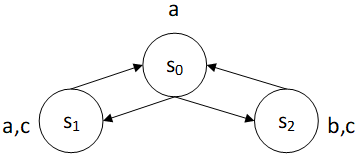
\includegraphics[width=5cm]{k1.png}\\
%  \caption{A simple Kripke structure}\label{Kripke_1}
%\end{figure}
%\end{example}

\begin{example}
Let $V=\{sr\}$ and $\overline V=\{sl,se,lc,le\}$ ($\Ha = V\cup \{sr\}$), and $\Hm$ is as illustrated in Figure~1.  We have $\Tr_0(s_0) \not \lrto_{\overline V} \Tr_0(s_1)$ and $\Tr_0(s_0) \not \lrto_{\overline V} \Tr_0(s_2)$, then $\dis_{\overline V}(\Hm, s_0, s_1, 0)$ and $\dis_{\overline V}(\Hm, s_0, s_2, 0)$.
Besides, it is easy checking that $s_1 \lrto_{\overline V} s_2$ since they have the same direct successor $s_0$.
Hence, $ch(\Hm, \overline V) = 0$.
Therefore, we have:
\begin{align*}
& {\cal F}_V(\Tr_0(s_0))= \neg sr \\
& {\cal F}_V(\Tr_0(s_1)) = {\cal F}_V(\Tr_0(s_2)) = sr, \text{ and then }\\
%\end{align*}
%Then we have,
%\begin{align*}
& {\cal F}_V (\Hm, s_0)= \neg sr \wedge \ALL\GLOBAL(\neg sr \rto  \ALL \NEXT sr)\wedge \ALL\GLOBAL(sr \rto  \ALL \NEXT \neg sr).
\end{align*}

%(2) Let $V=\{sl,se,lc,le\}$ and $\overline V=\{sr\}$. It is evident $\Tr_0(s_0) \not \lrto_{\overline V} \Tr_0(s_1)$ due to $L(s_0) -\overline V \neq L(s_1) -\overline V$, $\Tr_0(s_0) \not \lrto_{\overline V} \Tr_0(s_2)$ and $\Tr_0(s_1) \not \lrto_{\overline V} \Tr_0(s_2)$.
%And then we have $\dis_{\overline V}(\Hm,s_0,s_1,0)$, $\dis_{\overline V}(\Hm,s_0,s_2,0)$, $\dis_{\overline V}(\Hm,s_1,s_2,0)$ and $ch(\Hm, \overline V) = 0$.
%Therefore, we have:
%\begin{align*}
%&{\cal F}_V(\Tr_0(s_0)) = ls\wedge \neg se \wedge \neg lc \wedge \neg le\\
%&{\cal F}_V(\Tr_0(s_1)) = se \wedge lc \wedge \neg sl \wedge \neg le\\
%&{\cal F}_V(\Tr_0(s_2)) = le \wedge \neg sl \wedge \neg se \wedge \neg lc.
%\end{align*}
%Then it is easy to obtain ${\cal F}_V(\Hm, s_0)$ as above.
\end{example}

By the following theorem, we also have that given  $V\subseteq \Ha$, the characterizing formula of an initial \MPK-structure is unique (up to semantic equivalence) which describes this initial \MPK-structure on $V$.
\begin{theorem}\label{CF}
Given $V\subseteq \Ha$, let $\Hm=(S,R,L,s_0)$  and $\Hm'=(S',R', L',s_0')$ be two model structures. Then,
\begin{enumerate}[(i)]
 \item $(\Hm',s_0') \models {\cal F}_V({\cal M},s_0)
\text{ iff }
({\cal M},s_0) \lrto_{\overline V} ({\cal M}',s_0')$;

\item $s_0 \lrto_{\overline V} s_0'$ implies  ${\cal F}_V(\Hm, s_0) \equiv {\cal F}_V(\Hm', s_0')$.
\end{enumerate}

\end{theorem}

Moreover, we know that any initial \MPK-structure can be described as a \CTL\ formula from the definition of characterizing formula. Then,
\begin{lemma}\label{lem:models:formula}
  Let $\varphi$ be a formula. We have
  \begin{equation}
    \varphi\equiv \bigvee_{(\Hm, s_0)\in\Mod(\varphi)}{\cal F}_{\cal A}(\Hm, s_0).
\end{equation}
\end{lemma}
It follows that any \CTL\ formula  can rewritten in the form of a  characterizing formula (in the form of a disjunction of characterizing formulas; each corresponds to a single model.
%It follows that any \CTL\ formula can be described by the disjunction of the characterizing formulas of all the models of itself due to the number of models of a \CTL\ formula is finite.




%\begin{proof}
%This is following Lemma~\ref{lem:Vb:TrFormula:Equ} and the definition of the characterizing formula of initial \MPK-structure ${\cal K}$ on $V$.
%\end{proof}



\subsection{Semantic Properties of Forgetting in \CTL}
In this subsection we will give the definition of forgetting in \CTL\ and study it's semantic properties.
 We will first show via a representation theorem that our definition of forgetting correspond to the readily existing notion of forgetting which is characterised by several desirable properties (also called postulates) suggested in~\cite{Yan:AIJ:2009}. Next, we discuss various additional semantic properties of forgetting.

Now, we give the formal definition of forgetting in \CTL\ from the semantic point view.
\begin{definition}[Forgetting]\label{def:V:forgetting}
  Let $V\subseteq\cal A$ and $\phi$ a formula.
A formula $\psi$ with $\Var(\psi)\cap V=\emptyset$
is a {\em result of forgetting $V$ from} $\phi$, if
\begin{equation}
\resizebox{.91\linewidth}{!}{$
\displaystyle
  \Mod(\psi)=\{{\cal K}\mbox{ is initial}\mid \exists {\cal K}'\in\Mod(\phi)\ \&\ {\cal K}'\lrto_V{\cal K}\}.
  $}
\end{equation}
\end{definition}
Note that if both $\psi$ and $\psi'$ are results of forgetting $V$ from $\phi$, then
$\Mod(\psi)=\Mod(\psi')$, i.e., $\psi$ and $\psi'$ have the same models. In the sense
of equivalence, the forgetting result is unique (up to equivalence).
By Lemma~\ref{lem:models:formula}, such a formula always exists, which
is equivalent to
\begin{equation*}
  \bigvee_{{\cal K}\in  \{{\cal K}'\mid \exists {\cal K}''\in\Mod(\phi)\ \text{ and }\ {\cal K}''\lrto_V{\cal K}'\}} {\cal F}_{\overline V}({\cal K}).
\end{equation*}
For this reason, the forgetting result is denoted by $\CTLforget(\phi,V)$.

%By the definition of forgetting, we have

%\begin{proposition}\label{pro:IR_V:forget}
%Let $\varphi$ be a CTL formula and $V$ a set of atoms. If $V \cap \Var(\varphi) = {\O}$, then
%\[
%\CTLforget(\varphi,V) \equiv \varphi.
%\]
%\end{proposition}

%In the case $\psi$ is a result of forgetting $V$ from $\phi$, there are usually some
%expected properties (called {\em postulates}: (\W), (\PP), (\NgP) and (\textbf{IR})) for it~\cite{Yan:AIJ:2009}.
Assume you are given a formula $\varphi$, and $\varphi'$ is the formula after forgetting $V$, then we have the following desired properties, also called {\em postulates} of forgetting~\cite{Yan:AIJ:2009}.
\begin{itemize}
  \item Weakening (\W): $\varphi \models \varphi'$;
  \item Positive Persistence (\PP):
  Given $\eta \in \CTL$ if $\IR(\eta, V)$ and $\varphi \models \eta$, then $\varphi' \models \eta$;
  \item Negative Persistence (\NgP):   Given $\eta \in \CTL$  if $\IR(\eta, V)$ and $\varphi \nvDash \eta$, then $\varphi' \nvDash \eta$;
  \item Irrelevance (\textbf{IR}): $\IR(\varphi', V)$.
\end{itemize}

%lets explain them here

Intuitive enough, the postulate (\W) says, forgetting weakens the original formula.  (\PP)  and  (\NgP) correspond to the fact that so long as forgotten atoms $V$ are irrelevant to the remaining positive and the negative information, respectively, they do not affect such information. (\textbf{\IR}) states that forgotten atoms $V$ are not relevant for the final formula (i.e., $\varphi'$ is $V$-irrelevant).



\begin{theorem}[Representation Theorem]\label{thm:close}
Let $\varphi$, $\varphi'$ and $\phi$ be \CTL\ formulas and $V \subseteq \Ha$.
Then the following statements are equivalent:
\begin{enumerate}[(i)]
  \item $\varphi' \equiv \CTLforget(\varphi, V)$,
  \item $\varphi'\equiv \{\phi | \varphi \models \phi \text{ and } \IR(\phi, V)\}$,
  \item Postulates (\W), (\PP), (\NgP) and (\textbf{IR}) hold.
\end{enumerate}
\end{theorem}
The above theorem says that, the notion of forgetting  we defined, satisfies (and entailed by) the  four postulates of forgetting. Moreover, \CTL\ is closed under our definition of forgetting, i.e.,  for any CTL formula the result of forgetting is also a CTL formula.

\begin{lemma}\label{lem:KF:eq}
	Let $\varphi$ and $\alpha$ be two \CTL\ formulae and $q\in
		\overline{\Var(\varphi) \cup \Var(\alpha)}$. Then
	$\forget(\varphi \wedge (q\lrto\alpha), q)\equiv \varphi$.
\end{lemma}


\begin{proposition}\label{disTF}
Given a formula $\varphi \in \CTL$, $V$ a set of atoms and $p$ an atom such that $p \notin V$. Then,
\[
\CTLforget(\varphi, \{p\} \cup V) \equiv \CTLforget(\CTLforget(\varphi, p), V).
\]
\end{proposition}
This means that the result of forgetting $V$ from $\varphi$ can be obtained by forgetting atoms in $V$ one by one.
Moreover, the order of atoms does not matter (commutativity), which follows from  Proposition~\ref{disTF}.

\begin{corollary}[Commutativity]\label{disTFV}
Let $\varphi$ be a formula and $V_i\subseteq{\cal A}~(i=1,2)$. Then:
\[
\CTLforget(\varphi, V_1 \cup V_2) \equiv \CTLforget(\CTLforget(\varphi, V_1), V_2).
\]
\end{corollary}


The following results, which are satisfied in both classical propositional logic and modal logic \SFive~\cite{Yan:AIJ:2009}, further illustrate other essential semantic properties of forgetting.
\begin{proposition}\label{pro:ctl:forget:1}
Let $\varphi$, $\varphi_i$, $\psi_i$ ($i=1,2$) be formulas and $V\subseteq \Ha$. We have
\begin{enumerate}[(i)]
  \item $\CTLforget(\varphi, V)$ is satisfiable iff $\varphi$ is;
  \item If $\varphi_1 \equiv \varphi_2$, then $\CTLforget(\varphi_1, V) \equiv \CTLforget(\varphi_2, V)$;
  \item If $\varphi_1 \models \varphi_2$, then $\CTLforget(\varphi_1, V) \models \CTLforget(\varphi_2, V)$;
  \item $\CTLforget(\psi_1 \vee \psi_2, V) \equiv \CTLforget(\psi_1, V) \vee \CTLforget(\psi_2, V)$;
  \item $\CTLforget(\psi_1 \wedge \psi_2, V) \models \CTLforget(\psi_1, V) \wedge \CTLforget(\psi_2, V)$;
 % \item If $\IR(\psi_1, V)$, then $\CTLforget(\varphi \wedge \psi_1, V) \equiv \CTLforget(\varphi, V) \wedge \psi_1$.
\end{enumerate}
\end{proposition}


Another interesting result is that the forgetting of $Q T \varphi$ ($Q\in \{\EXIST, \ALL\}$, $T \in \{\FUTURE, \NEXT\}$) on $V\subseteq \Ha$ can be computed by $QT \CTLforget(\varphi, V)$. This gives us a convenient method to compute forgetting, since we can push the forgetting operator to a subformula without affecting the semantics, and rather compute the forgetting on this subformula.
\begin{proposition}[Homogeneity]\label{pro:ctl:forget:2}
  Let $V\subseteq\cal A$ and $\phi \in \CTL$,% and $Q\in \{\EXIST, \ALL\}$.
  \begin{enumerate}[(i)]
    \item $\CTLforget(\ALL\NEXT\phi,V)\equiv \ALL\NEXT \CTLforget(\phi,V)$.
    \item $\CTLforget(\EXIST\NEXT\phi,V)\equiv\EXIST\NEXT \CTLforget(\phi,V)$.
    \item $\CTLforget(\ALL \FUTURE\phi,V)\equiv \ALL \FUTURE \CTLforget(\phi,V)$.
    \item $\CTLforget(\EXIST\FUTURE\phi,V)\equiv\EXIST\FUTURE \CTLforget(\phi,V)$.
  \end{enumerate}
\end{proposition}



\subsection{Complexity Results}
In the following, we outline the computational complexity of the various tasks regarding the forgetting in \CTL\ and its popular fragment $\CTL_{\ALL\FUTURE}$.  It turns out that the model-checking on forgetting without any restriction is NP-complete.
%In this part we talk about the main complexity of entailment complexity of forgetting in \CTL.
\begin{proposition}[Model Checking on Forgetting]\label{modelChecking}
Let~$(\Hm,s_0)$ be an initial \MPK-structure, $\varphi$ be a \CTL\ formula and $V$ a set of atoms. Deciding whether $(\Hm,s_0)$ is a model of $\forget(\varphi, V )$ is NP-complete.
\end{proposition}
%\begin{proof}
%The problem can be determined by the following two things: (1) guessing
%an I-structure $\Hm',s_0'$ satisfying $\varphi$; and
%(2) checking if  $(\Hm, s_0) \leftrightarrow_V (\Hm', s_0')$. Both two steps can be done in polynomial time.
% Hence, the problem is in NP.
%The hardness follows that the model checking for propositional variable
%forgetting is NP-hard.
%\end{proof}

The fragment of \CTL, in which each formula contains only $\ALL \FUTURE$ temporal connective correspond to specifications that are desired to hold in all branches eventually. Such properties are of special interest in concurrent systems e.g., mutual exclusion and  waiting events~\cite{Baier:PMC:2008}.
In the following, we report various complexity results concerning forgetting and the logical entailment in this fragment.

\begin{theorem}[Entailment on Forgetting]\label{thm:comF}
Let $\varphi$ and $\psi$ be two $\CTL_{\ALL \FUTURE}$ formulas and $V$ a set of atoms. Then,
results:
\begin{enumerate}[(i)]
  \item deciding  $\forget(\varphi, V ) \models^? \psi$ is co-NP-complete,
  \item deciding  $\psi \models^? \forget(\varphi, V)$ is $\Pi_2^P$-complete,
  \item deciding $\forget(\varphi, V) \models^? \forget(\psi, V)$ is $\Pi_2^P$-complete.
\end{enumerate}
%Where $X\in\{\ALL, \EXIST\}$.
\end{theorem}
%\begin{proof}
%(1) It is proved that deciding whether $\psi$ is satisfiable is NP-Complete~\cite{DBLP:journals/ijfcs/MeierTVM15}. The hardness is easy to see by setting $\forget(\varphi, \Var(\varphi))$, i.e., deciding whether $\psi$ is valid.
%For membership, from Theorem
%3, we have $\forget(\varphi, V ) \models \psi$ iff $\varphi \models \psi$ and $IR(\psi, V )$.
%Clearly, in CTL($\ALL \FUTURE$), deciding $\varphi\models \psi$ is in co-NP. We show that deciding whether $IR(\psi, V )$ is also
%in co-NP. Without loss of generality, we assume that $\psi$ is satisfiable.
% %Then $\psi$ has a model in the polynomial size of $\psi$.
% We consider the complement of the problem: deciding whether $\psi$ is not irrelevant to $V$. It is easy to see that $\psi$ is
%not irrelevant to $V$ iff there exist a model $\Hm, s_0$ of $\psi$ and an
%initial \MPK-structure $\Hm',s_0'$  such that
%$\Hm, s_0 \leftrightarrow_V \Hm',s_0'$ and $\Hm',s_0'\nvDash \psi$. So checking whether $\psi$ is not irrelevant to $V$ can be achieved in the following steps: (1) guess two initial \MPK-structures $\Hm,s_0$ and $\Hm',s_0'$, (2) check if $\Hm,s_0 \models \psi$ and $\Hm',s_0'\nvDash \psi$, and (3) check
%$\Hm, s_0 \leftrightarrow_V \Hm',s_0'$. Obviously (1) can be done in polynomial time
%with a non-deterministic Turing machine while (2) and (3) can be done in polynomial time.
%
%(2) Membership. We consider the complement of the
%problem. We may guess an initial \MPK-structure $\Hm, s_0$ and check whether $\Hm,s_0 \models \psi$ and $\Hm,s_0$ $\nvDash \forget($ $\varphi$, $V)$. From Proposition~\ref{modelChecking}, we know that this is in $\Sigma_2^P$. So the original problem is in $\Pi_2^P$. Hardness. Let $\psi \equiv \top$. Then the problem is reduced to decide $\forget(\varphi, V )$'s validity. Since a propositional variable forgetting is a special case temporal forgetting, the hardness is directly followed from the proof of Proposition 24 in~\cite{DBLP:journals/jair/LangLM03}.
%
%(3) Membership. If $\forget(\varphi, V) \nvDash \forget(\psi, V)$ then there exist an initial \MPK-structure $\Hm, s$ such that $\Hm, s\models \forget(\varphi, V)$ but $\Hm, s \nvDash \forget(\psi, V)$, i.e.,, there is $\Hm_1, s_1 \lrto_V \Hm, s$ with $\Hm_1, s_1 \models \varphi$ but $\Hm_2, s_2 \nvDash \psi$ for every $\Hm_2, s_2$ with $\Hm, s \lrto_V \Hm_2, s_2$. It is evident that guessing such $\Hm, s$, $\Hm_1, s_1$ with $\Hm_1, s_1 \lrto_V \Hm, s$ and checking $\Hm_1, s_1\models \varphi$ are feasible while checking $\Hm_2, s_2 \nvDash \psi$ for every $\Hm, s \lrto_V \Hm_2, s_2$ can be done in polynomial time by call a nondeterministic Turing machine. Thus the problem is in $\Pi_2^P$.
%
%Hardness. It follows from (2) due to the fact that $\forget(\varphi, V) \models \forget(\psi, V)$ iff $\varphi \models \forget(\psi, V)$ thanks to $IR(\forget(\psi, V), V)$.
%
%\end{proof}

The following results follow from Theorem~\ref{thm:comF} and extends them to semantic equivalence.
\begin{corollary}
Let $\varphi$ and $\psi$ be two $\CTL_{\ALL \FUTURE}$ formulas and $V$ a set of atoms. Then
\begin{enumerate}[(i)]
  \item deciding $\psi \equiv^? \forget(\varphi, V)$ is $\Pi_2^P$-complete,
  \item deciding $\forget(\varphi, V) \equiv^? \varphi$ is co-NP-complete,
  \item deciding $\forget(\varphi, V) \equiv^? \forget(\psi, V)$ is $\Pi_2^P$-complete.
\end{enumerate}
\end{corollary}

\section{Strongest Necessary and Weakest Sufficient Conditions}
In this section, we will give the definitions of strongest necessary and weakest sufficient conditions (SNC and WSC, respectively) of a specification in \CTL\ and show that they can be obtained by forgetting under a given initial \MPK-structure and set $V$ of atoms.
We first start with defining these notions of an atomic proposition.
\begin{definition}[sufficient and necessary condition]\label{def:NC:SC}
Let $\phi$ be a formula (or an initial \MPK-structure), $\psi$ be a formula, $V \subseteq \Var(\phi)$, $q\in\Var(\phi)- V$
and $\Var(\psi)\subseteq V$.
\begin{itemize}
  \item $\psi$  is a {\em necessary condition} (NC in short) of $q$ on $V$ under $\phi$
    if $\phi \models q \rto \psi$.
  \item $\psi$  is a {\em sufficient condition} (SC in short) of $q$ on $V$ under $\phi$
    if $\phi \models \psi\rto q$.
  \item $\psi$  is a {\em strongest necessary condition} (SNC in short)
  of $q$ on $V$ under $\phi$
    if it is a NC of $q$ on $V$ under $\phi$ and $\phi\models\psi\rto\psi'$
    for any NC $\psi'$ of $q$ on $V$ under $\phi$.

    \item $\psi$  is a {\em weakest sufficient condition} (SNC in short)
  of $q$ on $V$ under $\phi$
    if it is a SC of $q$ on $V$ under $\phi$ and $\phi\models\psi'\rto\psi$
    for any SC $\psi'$ of $q$ on $V$ under $\phi$.
\end{itemize}
\end{definition}
Note that if both $\psi$ and $\psi'$ are SNC (WSC) of $q$ on $V$ under $\phi$, then
$\Mod(\psi)=\Mod(\psi')$, i.e., $\psi$ and $\psi'$ have the same models. In the sense
of equivalence the SNC (WSC) is unique (up to equivalence).



\begin{proposition}\label{dual}
(\textbf{dual})
 Let $V,q,\varphi$ and $\psi$ are like in Definition~\ref{def:NC:SC}.
 The $\psi$ is a SNC (WSC) of $q$ on $V$ under $\varphi$ iff $\neg \psi$ is a WSC (SNC)
    of $\neg q$ on $V$ under $\varphi$.
% \begin{enumerate}[(i)]
%   \item $\psi$ is a SNC of $q$ on $V$ under $\varphi$ iff $\neg \psi$ is a WSC
%    of $\neg q$ on $V$ under $\varphi$.
%   \item $\psi$ is a WSC of $q$ on $V$ under $\varphi$ iff $\neg \psi$ is a  SNC
%    of $\neg q$ on $V$ under $\varphi$.
% \end{enumerate}
\end{proposition}
This shows that the SNC and WSC are in fact dual conditions. Under this dual property, we can bother ourselves with only one of them e.g., SNC,  and WSC can be obtained easily. %\begin{proof}
%
%\end{proof}

In order to generalise Definition~\ref{def:NC:SC} to arbitrary formulas, one can replace $q$ (in the definition)  by any formula $\alpha$, and redefine  $V$ as a subset of $\Var(\alpha) \cup \Var(\phi)$.
%  For the case of formula, we have that the SCN (WSC) of any formula can be defined as follows:
%\begin{definition}\label{formulaNS}
   % Let $\Gamma$ be a formula or an initial \MPK-structure, $\alpha$ be a formula and $P\subseteq (\Var(\Gamma) \cup \Var(\alpha))$. A formula $\varphi$ of $P$ is  said to be a NC (SC) of $\alpha$ on $P$ under $\Gamma$ iff $\Gamma \models \alpha \rto \varphi$. It is said to be a SNC (WSC) if it is a NC (SC), and for any other NC (SC) $\varphi'$, we have that $\Gamma \models \varphi \rto \varphi'$ ($\Gamma \models \varphi' \rto \varphi$).
   % \end{definition}
    It turns out that the previous notion of SNC and WSC for an atomic proposition can be lifted to any formula, or conversely the SNC and WSC of any formula can be reduced to that of a proposition.
\begin{proposition}\label{formulaNS_to_p}
     Let $\Gamma$ and $\alpha$ be two formulas, $V \subseteq \Var(\alpha) \cup \Var(\phi)$  and $q$ is a new proposition not in $\Gamma$ and $\alpha$.
 Then, a formula $\varphi$ of $V$ is the SNC (WSC) of $\alpha$ on $V$ under  $\Gamma$ iff it is the SNC (WSC) of $q$ on $V$ under $\Gamma' = \Gamma \cup \{q \lrto \alpha\}$.
 \end{proposition}

The following result establishes the bridge between these two notions which are central to the paper; basically  SNC (WSC)  and the forgetting in which the former is obtained through the latter.



%In particular, it shows  how SNC  (WSC) of a property $q$ is obtained through the operation of forgetting.

\begin{theorem}\label{thm:SNC:WSC:forget}
 Let $\varphi$ be a formula, $V\subseteq\Var(\varphi)$ and $q\in\Var(\varphi)- V$.
 \begin{enumerate}[(i)]
   \item $\CTLforget (\varphi \land q$, $(\Var(\varphi) \cup \{q\}) - V)$
   is a SNC of $q$ on $V$ under $\varphi$.
   \item  $\neg\CTLforget (\varphi \land \neg q$, $(\Var(\varphi) \cup \{q\}) - V)$
   is a WSC of $q$ on $V$ under $\varphi$.
 \end{enumerate}
 \end{theorem}

As aforementioned, since any initial $\MPK$-structure can be characterized by a \CTL\ formula, we can obtain the SNC (and its dual WSC) of a target property (a formula) under an initial $\MPK$-structure by forgetting.
\begin{theorem}\label{thm:inK:SNC}
Let ${\cal K}= (\Hm, s)$ be an initial \MPK-structure with $\Hm=(S,R,L,s_0)$ on the set $\Ha$ of atoms, $V \subseteq \Ha$ and $q\in V' = \Ha - V$. Then:
 \begin{enumerate}[(i)]
   \item the SNC of $q$ on $V$ under ${\cal K}$ is $\CTLforget({\cal F}_{\Ha}({\cal K}) \wedge q, V')$.
   \item the WSC of $q$ on $V$ under ${\cal K}$ is $\neg \CTLforget({\cal F}_{\Ha}({\cal K}) \wedge \neg q, V')$.
 \end{enumerate}
\end{theorem}
%\label{thm:inK:SNC}\begin{proof}
%(i)
%As we know that any initial \MPK-structure ${\cal K}$ can be described as a characterizing formula ${\cal F}_{\Ha}({\cal K})$, then the SNC of $q$ on $V$ under ${\cal F}_{\Ha}({\cal K})$ is $\CTLforget({\cal F}_{\Ha}({\cal K}) \wedge q, \Ha - V)$. We will prove that $\CTLforget({\cal F}_{V \cup \{q\}}({\cal K}_{|V \cup \{q\}}) \wedge q, q)  \equiv  \CTLforget({\cal F}_{\Ha}({\cal K}) \wedge q, \Ha - V)$.
%
%($\Rto$) $\forall {\cal K}_1 \in \Mod(\CTLforget({\cal F}_{V \cup \{q\}}({\cal K}_{|V \cup \{q\}}) \wedge q, q))$\\
%$\Rto$ there is an initial \MPK-structure ${\cal K}'$ such that ${\cal K}' \models {\cal F}_{V \cup \{q\}}({\cal K}_{|V \cup \{q\}}) \wedge q$ and ${\cal K}_1 \lrto_{\{q\}} {\cal K}'$\\
%$\Rto$ ${\cal K}' \lrto_{\Ha-(V\cup \{q\})} {\cal K}_{|V \cup \{q\}}$  \hfill (Theorem~\ref{CF})\\
%$\Rto$ ${\cal K}_1 \lrto_{\Ha-V} {\cal K}_{|V \cup \{q\}}$   \hfill (Proposition~\ref{div})\\
%$\Rto$ ${\cal K}_{|V \cup \{q\}} \lrto_{\Ha-(V \cup \{q\})} {\cal K}$   \hfill  (Proposition~\ref{pro:VQ})\\
%$\Rto$ ${\cal K}' \lrto_{\Ha-(V\cup \{q\})} {\cal K}$  \hfill (Proposition~\ref{div})\\
%$\Rto$ ${\cal K} \models {\cal F}_{\Ha}({\cal K}) \wedge q$\\
%$\Rto$ ${\cal K}_1 \lrto_{\Ha -V} {\cal K}$\\
%$\Rto$ ${\cal K}_1 \models \CTLforget({\cal F}_{\Ha}({\cal K}) \wedge q, \Ha - V)$
%
%$(\Lto)$ $\forall {\cal K}_1 \in \Mod(\CTLforget({\cal F}_{\Ha}({\cal K}) \wedge q, \Ha - V))$ \\
%$\Rto$ there an initial \MPK-structure ${\cal K}_2$ \st\ ${\cal K}_2 \models {\cal F}_{\Ha}({\cal K}) \wedge q$ and ${\cal K}_1 \lrto_{\Ha - V} {\cal K}_2$\\
%$\Rto$ ${\cal K}_2 \lrto_{{\O}} {\cal K}$   \hfill (Theorem~\ref{CF})\\
%$\Rto$ ${\cal K}_2 \lrto_{\Ha-(V\cup \{q\})} {\cal K}_{|V \cup \{q\}}$ due to ${\cal K}_{|V \cup \{q\}} \lrto_{\Ha-(V \cup \{q\})} {\cal K}$   \hfill  (Proposition~\ref{pro:VQ})\\
%$\Rto$ ${\cal K}_2 \models {\cal F}_{V \cup \{q\}}({\cal K}_{|V \cup \{q\}}) \wedge q$  \\
%$\Rto$ ${\cal K}_1 \models \CTLforget({\cal F}_{V \cup \{q\}}({\cal K}_{|V \cup \{q\}}) \wedge q, q)$.
%
%(ii) This is proved by the dual property.
%\end{proof}

%\begin{example}
%For the Example~\ref{exmp:1}, the WSC of $\varphi$ on $V$ under ${\cal K} =(\Hm, s_0)$ is $\neg \CTLforget({\cal F}_{\Ha}({\cal K}) \wedge (q \lrto \varphi) \wedge \neg q, \Ha - V)$.
%\end{example}


\section{An Algorithm to Compute Forgetting}
\emph{Resolution} in \CTL\ is a method to decide the satisfiability of a \CTL\ formula.
In this part, we will explore a resolution-based method to compute forgetting in \CTL.
We use the transformation rules Trans(1) to Trans(12) and resolution rules (SRES1), \dots, (SRES8), RW1, RW2, (ERES1), (ERES2) in~\cite{zhang2009refined}.

The key problems of this method include (1) How to fill the gap between \CTL\ and $\CTLsnf$ since there is index for existential quantifier in $\CTLsnf$; and (2) How to eliminate the irrelevant atoms, which we want to forget, in the formula.
We will resolve these two problems by $\tuple{V,I}$-bisimulation and \emph{eliminate} operator respectively.
For convenient, we use $V\subseteq \Ha$ denote the set we want to forget, $V' \subseteq \Ha$ with $V \cap V'={\O}$ the set of atoms introduced in the transformation process below, $\varphi$  the \CTL\ formula, $T_{\varphi}$ be the set of $\CTLsnf$ clause obtained from $\varphi$ by using transformation rules  and $\Hm=(S,R,L,[\_], s_0)$ unless explicitly stated.
 Let $T$, $T'$ be two sets of formulae, $I$ a set of indexes and $V''\subseteq \Ha$, by $T\equiv_{\tuple{V'', I}} T'$ we mean that $\forall (\Hm, s_0) \in \Mod(T)$ there is a $(\Hm', s_0')$ such that $(\Hm,s_0) \lrto_{\tuple{V'', I}} (\Hm',s_0')$ and $(\Hm', s_0') \models T'$ and vice versa.







The algorithm of computing the forgetting in \CTL\ is as Algorithm~\ref{alg:compute:forgetting:by:Resolution}.
The main idea of this algorithm is to change the \CTL\ formula into a set of $\CTLsnf$ clauses at first (the Transform process), and then compute all the possible resolutions on the specified set of atoms (the Resolution process). Third, eliminating all the irrelevant atoms which dose not be eliminated by the resolution. We will describe this process, which include \emph{Instantiate}, \emph{Connect} and \emph{Removing\_atoms} sub-processes, in detail below.
Changing the result obtained before into a \CTL\ formula at last, this will include three sub-processes: \emph{Removing\_index} (removing the index in the formula), \emph{Replacing\_atoms} (replacing the atoms in $V'$ with an formula) and $T_\CTL$ (removing the $\start$ in the formula).
To describe our algorithm clearly, we illustrate it with the following example.
\begin{example}\label{main:examp}
Let $\varphi=\ALL((p\wedge q) \UNTIL (f\vee m)) \wedge r$ and $V=\{p\}$.
\end{example}
In the following context we will show how to compute the $\CTLforget(\varphi, V)$ step by step using our algorithm.


\begin{algorithm}[!h]
\caption{Computing forgetting based on Resolution}% ??????
\label{alg:compute:forgetting:by:Resolution}
%\LinesNumbered %?????????
\KwIn{A CTL formula $\varphi$ and a set $V$ of atoms}% ????????
\KwOut{$\emph{ERes}(\varphi, V)$}% ????
$T_{\varphi}={\O}$ // the initial set of $\CTLsnf$ clauses of $\varphi$ \;
%$T_{\NI} = {\O}$ // the set of $\CTLsnf$ clauses without index\;
$V'={\O}$ // the set of atoms introduced in the process of transforming $\varphi$ into $\CTLsnf$ clauses\;


$T_{\varphi}, V' \lto \emph{Transform}(\varphi)$ \;

$Res \lto \emph{Resolution}(T_{\varphi}, V')$  \;

$\Inst_{V'} \lto \emph{Instantiate}(Res, V')$ \;
$\Com_{\EXIST\FUTURE} \lto \emph{Connect}(\Inst_{V'})$ \;
$\emph{RemA} \lto \emph{Removing\_atoms}(\Com_{\EXIST\FUTURE}, \Inst_{V'})$\;
$\NI \lto \emph{Removing\_index}(\emph{RemA})$\;
$\Rp \lto \emph{Replacing\_atoms}(\NI)$ \;

\Return $\bigwedge_{\psi \in \Rp_{\CTL}} \psi$.
\end{algorithm}



%\begin{example}
%Let $\varphi=\ALL\GLOBAL \ALL\FUTURE (p \wedge r)$, $\Ha=\{p,r\}$ and $V=\{r\}$. For convenience, we use the label of a state to express the state and then remove the label function in a model structure.
%Let $\Hm_1=(\{\{p,r\}\}, \{(\{p,r\}, \{p,r\})\}, \{p,r\})$ and $\Hm_2=(\{\emptyset,\{p,r\}\}, \{(\emptyset, \{p,r\})$, $(\{p,r\}$, $\{p,r\})\}, \emptyset)$.
%\Hm_3=(\{\emptyset,\{p\}$, $\{p,r\}\}$, $\{(\emptyset$, $\{p\})$, $(\{p\}$, $\{p, r\})$, $(\{p, r\}$, $\emptyset)\}$, $\emptyset)$,
%The set of models of $\varphi$ is $\Mod(\varphi)=\{(\Hm_1, \{p\})$, $(\Hm_2$, $\emptyset), \dots\}$.

%Let $\Hm_1'=(\{\{p\}\}, \{(\{p\}, \{p\})\}, \{p\})$ and $\Hm_2'=(\{\emptyset,\{p\}\}, \{(\emptyset, \{p\})$, $(\{p\}$, $\{p\})\}, \emptyset)$
%  Then we can obtain all the possible initial \MPK-structure that is a model of $\CTLforget(\varphi, V)$, i.e., $\Mod(\CTLforget(\varphi, V)) =\{{\cal K}_1=(\Hm_1', \{p\}), {\cal K}_2=(\Hm_2', \emptyset), \dots\}$.

%Let $V'=\{p\}$, ${\cal K}_1=(\Hm_1, \{p,r\})$ and ${\cal K}_2=(\Hm_2, \emptyset)$, then
 %${\cal F}_{V'}({\cal K}_1)= p \wedge \ALL\GLOBAL (p\supset  \ALL \NEXT p)$,
 %and
% ${\cal F}_{V'}({\cal K}_2)=\neg p\wedge \ALL\GLOBAL (p\supset  \ALL \NEXT \neg p) \wedge \ALL\GLOBAL (\neg p\supset  \ALL \NEXT p)$. Similarly, we can obtain the characteristic formula of other models and then the $\CTLforget(\varphi, V)$.% is the disjunction of all the characteristic formulae of those models.
%\end{example}


\subsection{The Transform process}
The \emph{Transform} process, denoted as $\emph{Transform}(\varphi)$, is to transform the \CTL\ formula into a set of $\CTLsnf$ clauses by using the rules  Trans(1) to Trans(12) in~\cite{zhang2009refined}).
The transformation of an arbitrary \CTL\ formula into the set $T_{\varphi}$ is a sequence $T_0, T_1,\dots, T_n=T_{\varphi}$ of sets of formulae with $T_0=\{\ALL \GLOBAL(\start \supset p), \ALL \GLOBAL(p \supset \simp(\nnf(\varphi)))\}$ such that for every $i$ ($0 \leq i< n$), $T_{i+1} = (T_i \setminus \{\psi\}) \cup R_i$~\cite{zhang2009refined}), where $p$ is a new atom not appearing in $\varphi$, $\psi$ is a formula in $T_i$ not in $\CTLsnf$ clause and $R_i$ is the result set of applying a matching transformation rule to $\psi$. Note that throughout the transformation formulae are kept in negation normal form.
\begin{proposition}\label{pro:TranE}
 $\varphi \equiv_{\tuple{V', I}} T_{\varphi}$.
\end{proposition}
%\begin{proof} (sketch)
%This can be proved from $T_i$ to $T_{i+1}$ $(0\leq i < n)$ by using one transformation rule on $T_i$.

%We will prove this proposition from the following several aspects:
%
%(1) $\varphi \equiv_{\tuple{\{p\}, {\O}}} T_0$.
%
% $(\Rto)$ $\forall (\Hm_1,s_1) \in \Mod(\varphi)$, \ie $(\Hm_1,s_1) \models \varphi$. We can construct an \Ind-model structure $\Hm_2$ is identical to $\Hm_1$ except $L_2(s_2) = L_1(s_1) \cup \{p\}$. It is apparent that $(\Hm_2,s_2) \models T_0$ and $(\Hm_1, s_1) \lrto_{\tuple{\{p\}, {\O}}} (\Hm_2, s_2)$.
%
% $(\Lto)$ $\forall (\Hm_1,s_1) \in \Mod(T_0)$, it is apparent that $(\Hm_1,s_1) \models \varphi$ by the sematic of $\start$.
%
%By $\psi \rto_t R_i$ we mean using transformation rules $t$ on formula $\psi$ (the formulae $\psi$ as the
%premises of rule $t$) and obtaining the set  $R_i$ of transformation results. Let $X$ be a set of formulas
%we will show $T_i \equiv_{\tuple{V',I}} T_{i+1}$ by using the transformation rule $t$. Where $T_i= X \cup \{\psi\}$, $T_{i+1}=X \cup R_i$, $V'$ is the set of atoms introduced by $t$ and $I$ is the set of indexes introduced by $t$. (We will prove this result in $t\in \{$Trans(1), Trans(4), Trans(6)$\}$, other cases can be proved similarly.)
%
%(2) For $t$=Trans(1):\\
% $(\Rto)$ $\forall (\Hm_1,s_1) \in \Mod(T_i)$ \ie $(\Hm_1, s_1) \models X \wedge \ALL\GLOBAL(q \supset \EXIST \NEXT \varphi)$\\
% $\Rto$ $(\Hm_1,s_1)\models X$ and for every $\pi$ starting from $s_1$ and every state $s_1^j \in \pi$, $(\Hm,s_1^j) \models \neg q$ or there exists a path $\pi'$ starting from $s_1^j$ such that there exists a state $s_1^{j+1}$ such that $(s_1^j,s_1^{j+1})\in R_1$ and $(\Hm,s_1^{j+1})\models \varphi$\\
% We can construct an \Ind-model structure $\Hm_2$ is identical to $\Hm_1$ except  $[ind]_2= \bigcup_{s\in S} R_s \cup R_y$, where $R_{s_1^{j}}=\{(s_1^{j},s_1^{j+1}), (s_1^{j+1}, s_1^{j+2}),\dots\}$ and $R_y=\{(s_x,s_y)| \forall s_x \in S$ if $\forall (s_1',s_2')\in \bigcup_{s\in S} R_s, s_1'\neq s_x$ then find a unique $s_y\in S$ such that $(s_x,s_y)\in R\}$. It is apparent that $(\Hm_1, s_1) \lrto_{\tuple{{\O}, \{ind\}}} (\Hm_2, s_2)$ (let $s_2=s_1$).\\
% $\Rto$ for every path starting from $s_1$ and every state $s_1^j$ in this path, $(\Hm_2, s_1^j) \models \neg q$ or $(\Hm_2, s_1^j)\models \EXIST \NEXT \varphi_{\tuple{ind}}$ \hfill (by the semantic of $\EXIST \NEXT$)\\
% $\Rto$ $(\Hm_2, s_1) \models \ALL \GLOBAL(q \supset \EXIST_{\tuple{ind}} \NEXT \varphi )$\\
% $\Rto$ $(\Hm_2, s_1) \models X \wedge \ALL \GLOBAL(q \supset \EXIST_{\tuple{ind}} \NEXT \varphi )$
%
% $(\Lto)$ $\forall (\Hm_1,s_1) \in \Mod(T_{i+1})$ \ie $(\Hm_1,s_1) \models X \wedge \ALL \GLOBAL(q \supset \EXIST_{\tuple{ind}} \NEXT \varphi )$\\
% $\Rto$ $(\Hm_1,s_1) \models X$ and $(\Hm_1,s_1) \models \ALL \GLOBAL(q \supset \EXIST_{\tuple{ind}} \NEXT \varphi)$\\
% $\Rto$ for every path starting from $s_1$ and every state $s_1^j$ in this path, $(\Hm_1, s_1^j) \models \neg q$ or there exits a state $s'$ such that $(s_1^j, s')\in [ind]_1$ and $(\Hm_1, s') \models \varphi$ \hfill (by the semantic of $\EXIST_{\tuple{ind}} \NEXT$)\\
% $\Rto$ for every path starting from $s_1$ and every state $s_1^j$ in this path, $(\Hm_1, s_1^j) \models \neg q$ or $(\Hm_1, s_1^j) \models \EXIST \NEXT \varphi$ \hfill (by the semantic of $\EXIST \NEXT$)\\
% $\Rto$ $(\Hm_1,s_1) \models \ALL\GLOBAL(q \supset \EXIST \NEXT \varphi)$\\
% $\Rto$ $(\Hm_1, s_1) \models X \wedge \ALL\GLOBAL(q \supset \EXIST \NEXT \varphi)$\\
% It is apparent that $(\Hm_1, s_1) \lrto_{\tuple{{\O}, \{ind\}}} (\Hm_1, s_1)$.
%
%(3) For $t$=Trans(4):\\
% $(\Rto)$ $\forall (\Hm_1,s_1) \in \Mod(T_i)$, \ie $(\Hm_1,s_1) \models X \wedge \ALL\GLOBAL (q \supset \varphi_1 \vee \varphi_2)$ \\
% $\Rto$ $(\Hm_1,s_1) \models X$ and $\forall s_1'\in S, (\Hm_1,s_1') \models q \supset \varphi_1 \vee \varphi_2$\\
% $\Rto$ $(\Hm_1,s_1') \models \neg q$ or $(\Hm_1,s_1') \models \varphi_1 \vee \varphi_2$\\
% The we can construct an \Ind-model structure $\Hm_2$ as follows. $\Hm_2$ is the same with $\Hm_1$ when $(\Hm_1,s_1') \models \neg q$. When $(\Hm_1,s_1') \models q$, $\Hm_2$ is identical to $\Hm_1$ except if $(\Hm_1,s_1') \models \varphi_1$ then $L_2(s_1')= L_1(s_1')$ else $L_2(s_1') = L_1(s_1') \cup \{p\}$. It is apparent that $(\Hm_2,s_1') \models (q\supset \varphi_1 \vee p) \wedge (p \supset \varphi_2)$, then $(\Hm_2,s_1) \models T_{i+1}$ and $(\Hm_1, s_1) \lrto_{\tuple{\{p\}, {\O}}} (\Hm_2, s_2)$.
%
% $(\Lto)$ $\forall (\Hm_1, s_1) \in \Mod(T_{i+1})$, \ie $(\Hm_1,s_1) \models X \wedge \ALL\GLOBAL (q\supset \varphi_1 \vee p) \wedge \ALL\GLOBAL(p \supset \varphi_2)$. It is apparent that $(\Hm_1, s_1) \models T_i$.
%
%
%(4) For $t$=Trans(6):\\
%We prove for $\EXIST_{\tuple{ind}} \NEXT$, while for the $\ALL \NEXT$ can be proved similarly.
%
% $(\Rto)$ $\forall (\Hm_1,s_1) \in \Mod(T_i)$, \ie $(\Hm_1,s_1) \models X \wedge \ALL\GLOBAL(q \supset \EXIST_{\tuple{ind}}\NEXT \varphi)$\\
% $\Rto$ $(\Hm_1,s_1) \models X$ and $\forall s_1'\in S, (\Hm_1,s_1') \models q \supset \EXIST_{\tuple{ind}} \NEXT \varphi$\\
% $\Rto$ $(\Hm_1,s_1') \models \neg q$ or there exists a state $s'$ such that $(s_1', s') \in [ind]$ and $(\Hm_1,s') \models \varphi$ \\
% We can construct an \Ind-model structure $\Hm_2$ as follows. $\Hm_2$ is the same with $\Hm_1$ when $(\Hm_1,s_1') \models \neg q$. When $(\Hm_1,s_1') \models q$, $\Hm_2$ is identical to $\Hm_1$ except for $s'$ there is $L_2(s') = L_1(s') \cup \{p\}$. It is apparent that $(\Hm_2,s_1) \models \ALL\GLOBAL(q\supset \EXIST_{\tuple{ind}} \NEXT p) \wedge \ALL\GLOBAL(p \supset \varphi)$, $(\Hm_2,s_2) \models T_{i+1}$ and $(\Hm_1, s_1) \lrto_{\tuple{\{p\}, {\O}}} (\Hm_2, s_2)$ ($s_2=s_1$).
%
%  $(\Lto)$ $\forall (\Hm_1, s_1) \in \Mod(T_{i+1})$, \ie $(\Hm_1,s_1) \models X \wedge \ALL\GLOBAL(q\supset \EXIST_{\tuple{ind}} \NEXT p) \wedge \ALL\GLOBAL(p \supset \varphi)$. It is apparent that $(\Hm_1, s_1) \models T_i$.

%\end{proof}

This means that $\varphi$ has the same models with $T_{\varphi}$ excepting those atoms in $V'$ and those relations $[i]$ with $i\in I$.

\begin{example}\label{examp:Tran}
By the \emph{Transform} process, the result $T_{\varphi}$ of the Example~\ref{main:examp} can be listed as follows:
\begin{align*}
& 1. \start\supset z && 2. \top \supset \neg z \vee r && 3.\top \supset \neg x\vee f \vee m\\
& 4. \top \supset \neg z \vee x \vee y && 5.\top \supset \neg y \vee p && 6.\top \supset \neg y \vee q\\
& 7. z \supset \ALL \FUTURE x && 8. y \supset \ALL \NEXT(x\vee y).
\end{align*}
Besides, the set of new atoms introduced in this process is $V'=\{x, y,x\}$.
\end{example}



\subsection{The Resolution process}
The \emph{Resolution} process is to compute all the possible resolutions of $T_{\varphi}$ on $V\cup V'$, denoted as $\emph{Resolution}(T_{\varphi}, V\cup V')$.
A \emph{derivation} on a set $V\cup V'$ of atoms and $T_{\varphi}$ is a sequence $T_0, T_1, T_2$, $\dots$, $T_n=Res$ of sets of $\CTLsnf$ clauses such that $T_0 = T_{\varphi}$ and $T_{i+1} = T_i \cup R_i$ where $R_i$ is a set of clauses obtained as the conclusion of the application of a resolution rule to premises in $T_i$.
Note that all the $T_i$ ($0 \leq i \leq n$) are set of $\CTLsnf$ clauses.
Besides, if there is a $T_i$ containing $\start\supset \perp$ or $\top\supset \perp$, then we have $\CTLforget(\varphi, V)=\perp$.
%Given two clauses $C$ and $C'$, we call $C$ and $C'$ are resolvable, the result denote as $res(C,C')$, if there is a resolution rule using $C$ and $C'$ as the premises on some given atom.
%Then the pseudocode of algorithm Res is as Algorithm~\ref{alg:compute:Res}.

\begin{proposition}\label{pro:ResE}
$T_{\varphi} \equiv_{\tuple{V \cup V', {\O}}} Res$.
\end{proposition}
%\begin{proof}(sketch)
%This can be proved from $T_i$ to $T_{i+1}$ $(0\leq i < n)$ by using one resolution rule on $T_i$.
%%
%By $\psi \rto_r R_i$ we mean using resolution rules $r$ on set $\psi$ (the formulae in $\psi$ as the premises of rule $r$) and obtaining the set $R_i$ of resolution results.
%we will show $T_i \equiv_{\tuple{V,I}} T_{i+1}$ by using the resolution rule $r$. Where $T_i= X \cup \psi$, $T_{i+1}=X \cup R_i$, $X$ be a set of $\CTLsnf$ clauses, $p$ be the proposition corresponding with literal $l$ used to do resolution in $r$.
%
%(1) If $\psi \rto_r R_i$ by an application of $r\in \{\textbf{(SRES1)}, \dots, \textbf{(SRES8)}, \textbf{RW1}, \textbf{RW2}\}$, then $T_i \equiv_{\tuple{\{p\}, {\O}}} T_{i+1}$.
%
%
%On one hand, it is apparent that $\psi \models R_i$ and then $T_i \models T_{i+1}$. On the other hand, $T_i\subseteq T_{i+1}$ and then $T_{i+1} \models T_i$.
%
%(2) If $\psi \rto_r R_i$ by an application of $r=$\textbf{(ERES1)},
%then $T_i \equiv_{\tuple{\{l, w_{\neg l}^{\ALL}\}, {\O}}} T_{i+1}$.
%
%It has been proved that $\psi \models R_i$ in~\cite{bolotov2000clausal}, then there is $T_{i+1}=T_i \cup \Lambda_{\neg l}^{\ALL}$ and  then $\forall (\Hm_1,s_1) \in \Mod(T_i= X \cup \psi)$ there is a $(\Hm_2, s_2)\in \Mod(T_{i+1}=T_i \cup \Lambda_{\neg l}^{\ALL})$ s.t. $(\Hm_1, s_1) \lrto_{\tuple{\{p, w_{\neg l}^{\ALL}\}, {\O}}} (\Hm_2, s_2)$ and vice versa by Proposition~\ref{pro:TranE}.
%
%For rule \textbf{(ERES2)} we have the same result.
%\end{proof}

Proposition~\ref{pro:TranE} and Proposition~\ref{pro:ResE} mean that $\varphi \equiv_{\tuple{V \cup V', I}} Res$, this resolve part of the problem (1).

\begin{example}\label{examp:Res}
The resolution of $T_{\varphi}$ obtained from Example~\ref{examp:Tran} on $V\cup V'$ is as follows:
%\begin{align*}
%&(1) \start \supset r && (1,2,SRES 5)\\
%&(2) \start \supset x \vee y && (1,4,SRES 5)\\
%&(3) \top \supset \neg z \vee y \vee f \vee m && (3, 4, SRES 8)\\
%&(4) y \supset \ALL\NEXT(f\vee m\vee y) && (3,8, SRES 6)\\
%&(5) \top \supset \neg z \vee x \vee p && (4,5, SRES 8)\\
%&(6) \top \supset \neg z \vee x \vee q && (4,6, SRES 8)\\
%&(7) y \supset \ALL\NEXT(x\vee p) && (5, 7, SRES 6)\\
%&(8) y \supset \ALL\NEXT(x\vee q) && (5, 8, SRES 6)\\
%&(9) \start \supset f\vee m \vee y && (3,(2), SRES 5) \\
%&(10) \start \supset x \vee p && (5,(2),SRES 5) \\
%&(11) \start \supset x \vee q && (6,(2), SRES 5) \\
%&(12) \top \supset p \vee \neg z \vee f \vee m && (5,(3), SRES 8)\\
%&(13) \top \supset q \vee \neg z \vee f \vee m && (6,(3), SRES 8)\\
%&(14) y \supset \ALL\NEXT(p \vee f\vee m) && (5, (4), SRES 6) \\
%&(15) y \supset \ALL\NEXT(q \vee f\vee m) && (6, (4), SRES 6) \\
%&(16) \start \supset f\vee m \vee p && (5, (9), SRES 5) \\
%&(17) \start \supset f\vee m \vee q && (6, (9), SRES 5)
%\end{align*}
\begin{align*}
&\start \supset r &&  \start \supset x \vee y \\
& \top \supset \neg z \vee y \vee f \vee m && y \supset \ALL\NEXT(f\vee m\vee y)\\
& \top \supset \neg z \vee x \vee p &&  \top \supset \neg z \vee x \vee q \\
& y \supset \ALL\NEXT(x\vee p) && y \supset \ALL\NEXT(x\vee q)\\
& \start \supset f\vee m \vee y &&  \start \supset x \vee p \\
& \start \supset x \vee q && \top \supset p \vee \neg z \vee f \vee m \\
& \top \supset q \vee \neg z \vee f \vee m &&  y \supset \ALL\NEXT(p \vee f\vee m) \\
& y \supset \ALL\NEXT(q \vee f\vee m) &&  \start \supset f\vee m \vee p\\
& \start \supset f\vee m \vee q
\end{align*}
\end{example}


\subsection{The Elimination process}
For resolving problem (2), we should pay attention to the following properties that obtained from the transformation and resolution rules at first:
\begin{itemize}
  \item \textbf{(GNA)} for all atom $p$ in $\Var(\varphi)$, $p$ do not positively appear in the left hand of the $\CTLsnf$ clause;
  %\item \textbf{(CNI)} for each global clause, there must be an atom $p\in V'$ appearing in the right hand negatively;
  \item \textbf{(PI)} for each atom $p\in V'$, if $p$ appearing in the left hand of a $\CTLsnf$ clause, then $p$ appear positively.
\end{itemize}

This \emph{Elimination} process include three sub-processes: \emph{Instantiate}, \emph{Connect} and \emph{Removing\_atoms}. We will described those sub-processes carefully now.
\subsubsection{The Instantiation process}
An \emph{instantiate formula} $\psi$ of set $V''$ of atoms is a formula such that $\Var(\psi) \cap V'' ={\O}$.
Given a formula of the form $p \supset \psi$ with $p$ is an atom not in $V'' \cup \Var(\psi)$, if $\psi$ is an  instantiate formula of set $V''$ then we call $p$ is instantiated by $\psi$.
A key point to compute forgetting is eliminate those irrelevant atoms, for this purpose we define the follow instantiation process.
\begin{definition}\label{def:subst}
[instantiation] Let $V''=V'$ and $\Gamma=Res$, then the process of instantiation is as follows:
\begin{enumerate}[(i)]
  \item for each global clause $C= \top \supset D \vee \neg p \in \Gamma$, if there is one and on one atom $p \in V''\cap \Var(C)$  and $\Var(D) \cap (V \cup V'')= {\O}$ then let $C = p \supset D$ and $V'':=V''\setminus \{p\}$;
  \item find out all the possible instantiate formulae $\varphi_1, ..., \varphi_m$ of $V \cup V''$ in the $p\supset \varphi_i \in \Gamma$ ($1\leq i\leq m$);
  \item if there is $p\supset \varphi_i$ for some $i\in \{1,\dots, m\}$, then let $V'':=V''\setminus \{p\}$, which means $p$ is a instantiate formula;
  \item for $\bigwedge_{j=1}^m p_j \supset \varphi_i \in \Gamma$ ($i\in \{1,\dots, m\}$), if there is $\alpha \supset p_1,\dots, \alpha \supset p_m \in \Gamma$ then let $\Gamma_1 := \Gamma \cup \{\alpha \supset \varphi\}$. if $\Gamma_1\neq \Gamma$ then let $\Gamma:=\Gamma_1$ go to step (i), else return $V \cup V''$.
\end{enumerate}
Where $p, p_i$ ($1 \leq i\leq m$) are atoms and $\alpha$ is a conjunction of literals or $\start$.
\end{definition}

 We denote this process as $\emph{Instantiate}(\Gamma, V')$.
  After this process we obtain a set of atoms that do not has been instantiated by any instantiate formula of $V\cup V''$ in this process.

\begin{example}\label{exa:until:sub}
By using the instantiation process on result of Example~\ref{examp:Res}, we obtain that $x$ is instantiated by $f\vee m$ at first since there is $\top \supset \neg x \vee f \vee m \in T_{\varphi}$ with $x \in V'$ and $\Var(f \vee m) \cap (V\cup V') = \emptyset$, then $V''=\{y,z\}$.

Similarly, due to $\top \supset \neg y \vee q \in T_{\varphi}$ and $y \supset \ALL\NEXT(q \vee f\vee m)\in T_{\varphi}$, then $y$ can be instantiated by $q \wedge \ALL\NEXT(q \vee f\vee m)$. And $z$ can be instantiated by $r$. Therefore $V''=\emptyset$
%$r\wedge (f\vee m \vee q) \wedge q\wedge \ALL\NEXT(f\vee m\vee q) \wedge  (f\vee m \vee (q\wedge \ALL\NEXT(f\vee m\vee q))) \wedge \ALL\FUTURE(f \vee m)$.
That is $\emph{Instantiate}(T_{\varphi}^{r,V \cup V'}, V') = V$, which means all the introduced atoms are instantiated.
%Let $\varphi=\ALL((p\wedge q) \UNTIL (f\vee m)) \wedge r$ and $V=\{p\}$. Then we can compute $\Sub(T_{\varphi}^{r,V \cup V'}, V)$ as follows:
%
%At first, we transform $\varphi$ into a set of $\CTLsnf$ with $V'=\{x,y,z\}$, which is listed as:
%\begin{align*}
%& 1. \start\supset z && 2. \top \supset \neg z \vee r && 3.\top \supset \neg x\vee f \vee m\\
%& 4. \top \supset \neg z \vee x \vee y && 5.\top \supset \neg y \vee p && 6.\top \supset \neg y \vee q\\
%& 7. z \supset \ALL \FUTURE x && 8. y \supset \ALL \NEXT(x\vee y).
%\end{align*}
%
%In the second, we compute all the possible resolutions on $V\cup V'$ and is listed as:
%\begin{align*}
%&(1) \start \supset r && (2) \start \supset x \vee y &&(3) \top \supset \neg z \vee y \vee f \vee m \\
%& (4) y \supset \ALL\NEXT(f\vee m\vee y) &&(5) \top \neg z \vee x \vee p && (6) \top \neg z \vee x \vee q\\
%&(7) y \supset \ALL\NEXT(x\vee p) && (8) y \supset \ALL\NEXT(x\vee q) &&(9) \start \supset f\vee m \vee y \\
%& (10) \start \supset x \vee p &&(11) \start \supset x \vee q && (12) \top \supset p \vee \neg z \vee f \vee m \\
%&(13) \top \supset q \vee \neg z \vee f \vee m && (14) y \supset \ALL\NEXT(p \vee f\vee m) &&(15) y \supset \ALL\NEXT(q \vee f\vee m) \\
%& (16) \start \supset f\vee m \vee p &&(17) \start \supset f\vee m \vee q.
%\end{align*}

%By the process of instantiation we obtain that $y$ is instantiated by $q \wedge \ALL\NEXT(p \vee f\vee m)$, $x$ is instantiated by $f\vee m$ and $z$ is instantiated by $r$. That is $\Sub(T_{\varphi}^{r,V \cup V'}, V') = V$, which means all the introduced atoms are instantiated.
\end{example}

By instantiation operator, we guarantee those atoms in $V\cup V''$ are really irrelevant, \ie should be forgot.


\subsubsection{The Connect process}
Let $P$ be a conjunction of literals, $l$, $l_1$ be literals, in which $\Var(C_1)\cap V \cup V' = {\O}$, and $C_i$ ($i\in \{2,3,4\}$) be classical clauses.
 %Besides, by $l \supset \neg C_1 \vee C_2$ we mean the set $\{l \supset \neg C_{1,1} \vee C_2, \dots, l \supset \neg C_{1,x} \vee C_2$, where $C_{1,i}$ is a literal appearing in $C_1$.
%As we can see that those exist resolution rules cannot deduct all the possible result, so we add following new rules:
Let $A=\{l \supset \neg l_1 \vee C_2, l \supset C_3\vee C_2\}$, $\alpha=P \supset ((\neg C_3 \wedge \neg C_2) \supset  (\EXIST_{\tuple{ind}}\NEXT(C_3 \wedge \neg (C_2 \vee C_4) \supset \ALL\NEXT \ALL\FUTURE(C_3 \vee C_2))))$ and $\beta = P \supset ((\neg C_3 \wedge \neg C_2) \supset (\ALL\NEXT(C_3 \wedge  \neg (C_2 \vee C_4) \supset \ALL\NEXT \ALL\FUTURE(C_3 \vee C_2))))$,we add following new rules, we call it \textbf{EF} imply.
\begin{align*}
& \textbf{(EF1)} \{P\supset \ALL\FUTURE l, P\supset \EXIST_{\tuple{ind}}\NEXT (l_1 \vee C_4)\}\cup A \rto \alpha \\
%&  \qquad \rto\{P \supset ((\neg C_3 \wedge \neg C_2) \supset  (\EXIST_{\tuple{ind}}\NEXT(C_3 \wedge \neg (C_2 \vee C_4) \supset \ALL\NEXT \ALL\FUTURE(C_3 \vee C_2))))\},\\
& \textbf{(EF2)} \{P\supset \ALL\FUTURE l, P\supset \ALL \NEXT (l_1 \vee C_4)\}\cup A \rto \beta \\
%& \qquad \rto \{ P \supset ((\neg C_3 \wedge \neg C_2) \supset (\ALL\NEXT(C_3 \wedge  \neg (C_2 \vee C_4) \supset \ALL\NEXT \ALL\FUTURE(C_3 \vee C_2))))\}\\
& \textbf{(EF3)} \{P\supset \EXIST_{\tuple{ind}}\FUTURE l, P\supset \EXIST_{\tuple{ind}}\NEXT (l_1 \vee C_4)\}\cup A \rto \alpha  \\
%& \qquad \rto \{P \supset ((\neg C_3 \wedge \neg C_2) \supset (\EXIST_{\tuple{ind}}\NEXT(C_3 \wedge  \neg (C_2 \vee C_4) \supset \ALL\NEXT \ALL\FUTURE(C_3 \vee C_2))))\},\\
& \textbf{(EF4)} \{P\supset \EXIST_{\tuple{ind}}\FUTURE l, P\supset \ALL\NEXT (l_1 \vee C_4)\}\cup A \rto \alpha
\end{align*}



By $\emph{Connect}(\emph{Instantiate}(Res, V'))$ we mean using (EF1) to (EF4) on $Res$ and replacing $P\supset \ALL\NEXT (\neg l \vee C_2 \vee C_4)$ with $P\supset \ALL\NEXT (\neg l \vee C_2 \vee C_4) \vee \beta$ for rule (EF2) and replacing $P\supset \EXIST_{\tuple{ind}}\NEXT (\neg l \vee C_2 \vee C_4)$ with $P\supset \EXIST_{\tuple{ind}}\NEXT (\neg l \vee C_2 \vee C_4) \vee \alpha$ for other rules when $l$, $C_2$, $C_3$  and $C_4$ are instantiate formulae of  $\Sub(Res, V')$ and $\Var(l_1) \in V\cup V'$.


\begin{proposition} \label{pro:EF}
Let $\Gamma=Res$, we have $\Gamma \equiv_{\tuple{V', {\O}}}\emph{Connect}(\emph{Instantiate}(\Gamma, V'))$.
\end{proposition}
%\begin{proof}
%It is obvious from the  \textbf{(EF1)} to \textbf{(EF4)}.
%
%We prove the (EF1), for other rules can be proved similarly.
%Let $T_{i+1}=T_i \cup \{\varphi\}$, where $\{\varphi\}$ is obtained from $T_i$ by using rule (EF1) on $T_i$, \ie $\varphi =P \supset ((\neg C_3 \wedge \neg C_2) \supset  (\EXIST_{\tuple{ind}}\NEXT(C_3 \wedge \neg (C_2 \vee C_4) \supset \ALL\NEXT \ALL\FUTURE(C_3 \vee C_2))))$.
%It is apparent that $T_{i+1} \models T_i$ and $T_i \models P\supset \EXIST_{\tuple{ind}}\NEXT (\neg l \vee C_2 \vee C_4)$.
%We will show that $\forall (\Hm, s_0) \in \Mod(T_i)$ there is an initial Ind-structure $(\Hm',s_0')$ such that $(\Hm',s_0') \models T_{i+1}$ and $(\Hm',s_0') \lrto_{\tuple{V', {\O}}} (\Hm, s_0)$
%
%$\forall (\Hm, s) \models T_i$ we suppose $(\Hm, s) \models P \wedge \neg C_3 \wedge \neg C_2$ and $(\Hm, s_1)\models C_3 \wedge \neg C_2 \wedge \neg C_4$ with $(s, s_1) \in [ind]$ (due to other case can be proved easily).
%Then we have $(\Hm, s) \nvDash l$ (by $(\Hm, s) \models l \supset C_3 \vee C_2$) and $(\Hm,s_1) \models l_1$ (by $(\Hm, s) \models P\supset \EXIST_{\tuple{ind}}\NEXT (l_1 \vee C_4)$).
%If $(\Hm,s_1) \nvDash \ALL\NEXT \ALL\FUTURE(C_3 \vee C_2)$ then we have $(\Hm, s_1) \models l$ due to $(\Hm, s) \models \ALL\GLOBAL(l\supset C_3 \vee C_2)$ and $(\Hm, s)\models \ALL\FUTURE l$.
%And then $(\Hm, s_1) \models \neg l_1$ by $(\Hm,s) \models \ALL \GLOBAL(l\supset \neg l_1 \vee C_2)$.
%It is contract with our supposing.
%Then $(\Hm,s_1) \models \ALL\NEXT \ALL\FUTURE(C_3 \vee C_2)$.
%
%%By Proposition~\ref{pro:TranE} we have $\forall (\Hm, s) \in \Mod(\varphi)$ there is an initial Ind-structure $(\Hm',s')$ such that $(\Hm', s')\models T_{\varphi}$ and $(\Hm,s) \lrto_{\tuple{V_F, \emptyset}} (\Hm, s)$.
%
%\end{proof}


\subsubsection{The Removing\_atoms process}
For eliminate those irrelevant atoms, we can do the following elimination operator.
\begin{definition}[Removing\_atoms]\label{def:Elm}
%\textbf{(Elimination)}
Let $T$ be a set of formulae, $C \in T$ and $V$ a set of atoms, then the elimination operator is defined as:
$$ \emph{Removing\_atoms}(C, V)=\left\{
\begin{aligned}
\top, && if\ \Var(C) \cap V \neq {\O} \\
C, && else.
\end{aligned}
\right.
$$
\end{definition}
For convenience, for any set $T$ of formula we have $\emph{Removing\_atoms}(T, V) = \{\emph{Removing\_atoms}(r, V) | r \in T\}$.




\begin{proposition}\label{pro:elm}
Let $V''=V \cup V'$, $\Gamma=\emph{Instantiate}(Res, V')$ and $\Gamma_1=\emph{Removing\_atoms}$ $(\emph{Connect}(\Gamma), \Gamma)$, then  $\Gamma_1\equiv_{\tuple{V\cup V', {\O}}} Res$ and $\Gamma_1 \equiv_{\tuple{V \cup V', I}} \varphi$.
\end{proposition}
%\begin{proof}
%Note the fact that for each clause $C = T \supset H$ in $\emph{Connect}(\Gamma)$, if $\Gamma \cap \Var(C) \neq \emptyset$ then there must be an atom $p\in \Gamma \cap \Var(H)$. It is apparent that $\emph{Connect}(\Gamma) \models \Gamma_1$, we will show $\forall (\Hm, s_0) \in \Mod(\Gamma_1)$ there is a $(\Hm', s_0)$ such that $(\Hm', s_0) \models \emph{Connect}(\Gamma)$ and $(\Hm, s_0) \lrto_{\tuple{\Gamma, \emptyset}} (\Hm', s_0)$.
%Let $C = T \supset H$ in $\emph{Connect}(\Gamma)$ with $\Gamma \cap \Var(C) \neq \emptyset$,
%$\forall (\Hm, s_0) \in \Mod(\Gamma_1)$ we construct $(\Hm', s_0)$ as $(\Hm, s_0)$ except
%%We will proof this proposition from the following two points.
% for each $s\in S$, if $(\Hm, s) \nvDash T$ then $L'(s) = L(s)$, else:
%\begin{enumerate}[(i)]
%  \item if $(\Hm,s) \models H$, then $L'(s) = L(s)$;
%  \item else if $(\Hm, s) \models T$ with $p \in \Var(H)\cap V$, then if $p$ appearing in $H$ negatively, then if $C$ is a global (or an initial) clause then let $L'(s) = L(s) \setminus \{p\}$ else let $L'(s_1) = L(s_1) \setminus \{p\}$ for (each (if $C$ is an $\ALL$-step or $\ALL$-sometime clause)) $(s,s_1) \in R$, else if $C$ is a global (or an initial) clause then let $L'(s) = L(s) \cup \{p\}$ else let $L'(s_1) = L(s_1) \cup \{p\}$ for (each (if $C$ is a $\ALL$-step or $\ALL$-sometime clause)) $(s,s_1) \in R$.
%  \item for other clause $C=Q\supset H$ with $p\in \Var(H)\cap \Gamma$, we can do it as (ii).
%\end{enumerate}
%
%It is apparent that $(\Hm, s_0) \lrto_{\tuple{\Gamma, \emptyset}} (\Hm', s_0)$, we will show that $(\Hm', s_0) \models \emph{Connect}(\Gamma)$ from the following two points:
%\begin{enumerate}[(1)]
%  \item For (ii) talked-above, we show it from the form of $\CTLsnf$ clauses. Supposing $C_1$ and $C_2$ are instantiate formula of $\Gamma$:
%  \begin{enumerate}[(a)]
%    \item If $C$ is a global clause, i.e. $C=\top \supset p \vee C_1$ with $C_1$ is a disjunction of literals (we suppose $p$ appearing in $C$ positively). If there is a $C'=\top \supset \neg p \vee C_2 \in \emph{Connect}(\Gamma)$, then there is $\top \supset C_1 \vee C_2 \in \emph{Connect}(\Gamma)$ by the resolution ($(\Hm,s) \models C_2$ due to we have suppose $(\Hm,s) \nvDash C$). It is apparent that $(\Hm', s_0) \models C \wedge C'$.
%    \item If $C = T \supset \EXIST_{\tuple{ind}}\NEXT (p \vee C_1)$.
%    %We talk about the case that $(\Hm,s)\models T$ and $(\Hm,s)\nvDash \EXIST_{\tuple{ind}}\NEXT (p \vee C_1)$
%        If there is a $C'=T' \supset \EXIST_{\tuple{ind}}\NEXT( \neg p \vee C_2) \in \emph{Connect}(\Gamma)$, then there is $T\wedge T' \supset \EXIST_{\tuple{ind}}\NEXT(C_1 \vee C_2) \in \emph{Connect}(\Gamma)$  by the resolution ($(\Hm,s) \models \EXIST_{\tuple{ind}}\NEXT C_2$ due to we have suppose $(\Hm,s) \nvDash C$). It is apparent that $(\Hm', s_0) \models C \wedge C'$.
%    \item Other cases can be proved similarly.
%  \end{enumerate}
%
%  \item (iii) can be proved as (ii) due to the fact we point at the beginning.
%\end{enumerate}
%Therefore, we have $\Gamma_1\equiv_{\tuple{V\cup V', {\O}}} T_{\varphi}^{r, V''}$  by Proposition~\ref{pro:VI:div} and Proposition~\ref{pro:EF}.
%
%And then $\Gamma_1 \equiv_{\tuple{V \cup V', I}} \varphi$ follows.
%\end{proof}


\begin{example}\label{examp:remA}
After removing the clauses that include atoms in $V=\{p\}$, the following clauses have been left:
\begin{align*}
& \start\supset z &&  \top \supset \neg z \vee r && \top \supset \neg x\vee f \vee m\\
&  \top \supset \neg z \vee x \vee y &&  \start \supset f\vee m \vee q &&  \top \supset \neg y \vee q\\
&  z \supset \ALL \FUTURE x &&   y \supset \ALL \NEXT(x\vee y) && \start \supset r \\
& \start \supset x \vee y && \top \supset \neg z \vee y \vee f \vee m && y \supset \ALL\NEXT(f\vee m\vee y)\\
& \top \supset \neg z \vee x \vee q && y \supset \ALL\NEXT(x\vee q) &&  \start \supset f\vee m \vee y \\
& \start \supset x \vee q && \top \supset q \vee \neg z \vee f \vee m && y \supset \ALL\NEXT(q \vee f\vee m)
\end{align*}
\end{example}


\subsection{Remove the Index and \start}
The $\emph{Removing\_index}(\emph{RemA})$ process is to change the set $\emph{RemA}$ obtained above into a set of formulas without the index by using the equations in Proposition~\ref{pro:In2NI}.
%The following proposition is important for our algorithm since ... .
\begin{proposition}\label{pro:In2NI}
Let $P$, $P_i$ and $\varphi_i$ be \CTL\ formulas, then
\begin{enumerate}[(i)]
  \item $\bigwedge_{i=1}^n P\supset \EXIST_{\tuple{ind}} \NEXT \varphi_i   \equiv_{\tuple{\emptyset, \{ind\}}} P\supset \EXIST \NEXT \bigwedge_{i=1}^n \varphi_i$,
  \item $\bigwedge_{i=1}^n P_i\supset \EXIST_{\tuple{ind}} \NEXT \varphi_i \equiv_{\tuple{\emptyset, \{ind\}}} \bigwedge_{e \in 2^{\{0,\dots, n\}} \setminus \{\emptyset\}}(\bigwedge_{i\in e}P_i\supset \EXIST \NEXT (\bigwedge_{i\in e}\varphi_i))$,
  \item $\bigwedge_{i=1}^n P\supset \EXIST_{\tuple{ind}} \FUTURE \varphi_i  \equiv_{\tuple{\emptyset, \{ind\}}} P\supset \bigvee\EXIST\FUTURE (\varphi_{j_1} \wedge \EXIST\FUTURE(\varphi_{j_2} \wedge \EXIST\FUTURE(\dots \wedge \EXIST\FUTURE \varphi_{j_n})))$, where $(j_1, \dots, j_n)$ are sequences of all elements in $\{0, \dots, n\}$,
  \item $P\supset (C \vee \EXIST_{\tuple{ind}} \NEXT \varphi_1) \wedge P \supset \EXIST_{\tuple{ind}} \NEXT \varphi_2 \equiv_{\tuple{\emptyset, \{ind\}}} P \supset ((C \wedge \EXIST \NEXT \varphi_2) \vee \EXIST \NEXT (\varphi_1 \wedge \varphi_2))$,
  \item $P\supset (C \vee \EXIST_{\tuple{ind}} \NEXT \varphi_1) \vee P \supset \EXIST_{\tuple{ind}} \NEXT \varphi_2 \equiv_{\tuple{\emptyset, \{ind\}}} P \supset (C \vee \EXIST \NEXT (\varphi_1 \vee \varphi_2))$.
\end{enumerate}
\end{proposition}
%\begin{proof}
%It is easy to check.
%\end{proof}

\begin{lemma}\label{lem:No:Ind}
\textbf{(NI-BRemain)}
%Let $T'=\emph{Removing\_index}(\emph{RemA})$.
Let $I$ is the set of indexes in $\emph{RemA}$,
we have $\emph{RemA}\equiv_{\tuple{{\O}, I}} \emph{Removing\_index}(\emph{RemA})$.
%Then $\forall (\Hm,s_0) \in \Mod(T)$ there is a $(\Hm',s_0') \in \Mod(T')$ such that $(\Hm,s_0) \lrto_{\tuple{{\O}, I}} (\Hm',s_0')$ and vice versa.
%where $I$ is the set of indexes in $\emph{RemA}$.
\end{lemma}
%\begin{proof}
%It is easy checking that from the definition of $\emph{Removing\_index}$.
%\end{proof}

In our Example~\ref{examp:remA} we do not need this process due to there is no index in the set of formulae.
%\subsection{Remove the \start}
Let $T$ be a set of $\CTLsnf$ clauses, then we define the following operator:
\begin{align*}
&T_{\CTL} = \{C|C'\in T\ \mbox{and}\ C = D \ \mbox{if}\ C' \mbox{is the form}\\
& \ALL\GLOBAL(\start\supset D), \mbox{else}\ C= C'\}.
\end{align*}
Then $T \equiv T_{\CTL}$ by $\varphi \equiv \ALL \GLOBAL (\start \supset \varphi)$~\cite{bolotov2000clausal}.


The last step of our algorithm is to eliminate all the atoms in $V'$ which has been introduced in the \emph{Transform} process. Let $V''=V \cup V'$, $\Gamma=\emph{Instantiate}(Res, V')$ and $\Gamma_1=\emph{Removing\_atoms} (\emph{Connect}(\Gamma))$, then $\emph{Replacing\_atoms}(\emph{Removing\_index}(\Gamma_1))$ is obtained from $\emph{Removing\_index}(\Gamma_1)$ by doing the following two steps for each $p\in (V'\setminus \Gamma)$:
\begin{itemize}
  \item replacing each $p\supset \varphi_1\vee \dots \vee p \supset \varphi_n$ with $p \supset \bigvee_{i=1}^n \varphi_i$;
  \item replacing $p\supset \varphi_{1}\wedge \dots \wedge p \supset \varphi_{m}$ with $\varphi_j$ are instantiate formulae of  $\Gamma$ $(j \in \{1,\dots, m\})$ with $p \lrto \psi$, where $\psi=\bigwedge_{j=1}^{m} \varphi_{j}$ and $p$ do not appear in $\varphi_j$, .
  \item For other formula $C\in \Gamma_1$, replacing every $p$ in $C$ with $\psi$.
\end{itemize}
%Where $\NI(S)$ means do $\NI(e)$ for each $e\in S$ with $S$ is a set of sets of $\CTLsnf$ clause.
Apparently, this process is just a process of replacing each atom with an equivalent formula. Then we have:
\begin{proposition}
Let $\Gamma_1=\emph{Instantiate}(Res, V')$, $\Gamma_2 =\emph{Removing\_atoms}$ $(\emph{Connect}(\Gamma_1), \Gamma_1)$ and $\Gamma_3 = \emph{Replacing\_atoms}(\emph{Removing\_index}(\Gamma_2))$, then $\Gamma_2  \equiv_{\tuple{V'\setminus \Gamma_1, I}} \Gamma_3$ and $\varphi \equiv_{\tuple{V\cup V', \emptyset}}$ $(\Gamma_3)_{CTL}$.
\end{proposition}
%\begin{proof}
%For each $p$ talked above is a name of the formula $\psi$, \ie $p \lrto \psi$.
%Then $\Gamma_2  \equiv_{\tuple{(V'\setminus \Gamma_1), I}} \Gamma_3$, and then $\Gamma_2 \equiv_{\tuple{V\cup V', I}} \Gamma_3$  by (V) of Proposition~\ref{div}.
%
%Therefore, $\varphi \equiv_{\tuple{V\cup V', \emptyset}} (\Gamma_3)_{CTL}$ by Proposition~\ref{pro:elm} and the definitions of $\emph{Removing\_index}$ and $T_{\CTL}$.
%\end{proof}


\begin{example}\label{exa:replace:sub}
By using the \emph{Replacing\_atoms} process on result of Example~\ref{examp:remA} directly since there is not index in those clauses, we obtain that $x$ is replaced by $f\vee m$ at first, then $y$ is replaced by $q \wedge \ALL\NEXT(q \vee f\vee m)$ and $z$ is replaced by $r\wedge (f\vee m \vee q) \wedge (f\vee m \vee (q\wedge \ALL\NEXT(f\vee m\vee q))) \wedge \ALL\FUTURE(f \vee m)$.
\end{example}




\subsection{The Correction and Complexity of the Algorithm}
In the case that formula dose not include index, we use model structure $\Hm=(S,R,L, s_0)$ to interpret formula instead of \Ind-model structure. 
%Therefore it is apparent that $\forall (\Hm,s_0) \in \Mod(\varphi)$ there is a $(\Hm',s_0') \in \Mod(\Gamma_1)$ such that $(\Hm,s_0) \lrto_{V \cup V'} (\Hm',s_0')$ and vice versa.


\begin{theorem}[Resolution-based CTL-forgetting]\label{thm:Res_based:V_CTLforget}
Let $V''=V \cup V'$ and $\Gamma_1=\emph{ERes}(\varphi,V)$, then %R(\NI(\Elm(\EXIST\FUTURE(\Gamma),\Gamma)))_{\CTL}$, then
\begin{enumerate}[(i)]
\item $\CTLforget(\varphi, V'') \equiv \Gamma_1$;
\item $\CTLforget(\varphi, V) \equiv \bigwedge_{\psi \in \Gamma_1} \psi$.
\end{enumerate}
\end{theorem}
%\begin{proof}
% ($\Rto$) $\forall (\Hm,s_0) \in \Mod(\CTLforget(\varphi, V' \cup V))$\\
% $\Rto$ $\exists (\Hm',s_0') \in \Mod(\varphi)$ s.t. $(\Hm,s_0) \lrto_{V'\cup V} (\Hm', s_0')$\\
% $\Rto$ $\exists (\Hm_1, s_1) \in \Mod(\Gamma_1)$ s.t. $(\Hm_1,s_1) \lrto_{V'\cup V} (\Hm', s_0')$\\
% $\Rto$ $(\Hm,s_0) \lrto_{V'\cup V} (\Hm_1,s_1)$\\
% $\Rto$ $(\Hm,s_0) \models \Gamma_1$ \hfill ($\IR(\Gamma_1, V \cup V')$)
%
% ($\Lto$)$\forall (\Hm_1, s_1) \in \Mod(\Gamma_1)$\\
% $\Rto$ $\exists (\Hm',s_0') \in \Mod(\varphi)$ s.t. $(\Hm_1,s_1) \lrto_{V'\cup V} (\Hm', s_0')$ \\
% $\Rto$ $(\Hm_1, s_1) \models \CTLforget(\varphi, V' \cup V)$ \hfill ($\IR(\CTLforget(\varphi, V' \cup V), V \cup V')$ and $\varphi \models \CTLforget(\varphi, V' \cup V)$)
%\end{proof}

%Then we have the following result:
%\begin{theorem}\label{thm:Res_based:CTLforget}
%\textbf{(Resolution-based CTL-forgetting)}
%Let $\Gamma_1=\emph{ERes}(\varphi, V)$, then
%\[
%\CTLforget(\varphi, V) \equiv \bigwedge_{\psi \in \Gamma_1} \psi.
%\]
%\end{theorem}
%
%We can obtain that $\CTLforget(\varphi, V) \equiv \CTLforget(\varphi, V' \cup V)$ by Theorem~\ref{thm:Res_based:V_CTLforget} since $\varphi$ is irrelevant with $V'$. Therefore, the Theorem~\ref{thm:Res_based:CTLforget} is proved.

Then we can obtain the result of forgetting of Example~\ref{exa:until:sub}:
\begin{align*}
& \CTLforget(\varphi, \{p\}) \equiv r\wedge (f\vee m \vee q)  \wedge  \ALL\FUTURE(f \vee m) \wedge\\
& (f\vee m \vee (q\wedge \ALL\NEXT(f\vee m\vee q)))  \wedge \ALL\GLOBAL((q\wedge \ALL\NEXT(f\vee m\vee q)\\
& \supset \ALL\NEXT(f\vee m \vee (q\wedge \ALL\NEXT(f\vee m\vee q))))).
\end{align*}

\begin{example}
Consider the model given in Figure 1. Assume that we are given a property $\alpha = \ALL\GLOBAL\EXIST\FUTURE(lc \wedge sr)$ and $\{ lc\}$. Then, it is easy to check that $\CTLforget(\alpha,\{ lc\}) \equiv \ALL\GLOBAL\EXIST\FUTURE sr$.
\end{example}


\begin{proposition}
Let $\varphi$ be a CTL formula and $V \subseteq \Ha$.
The time and space complexity of Algorithm~\ref{alg:compute:forgetting:by:Resolution} are $O((m+1)2^{4(n+n')}$. Where $|\Var(\varphi)|=n$, $|V'|=n'$ ($V'$ is set of atoms introduced in transformation) and $m$ is the number of the set $Ind$ of indices introduced during transformation.
\end{proposition}
%\begin{proof}
%It follows from the \emph{Resolution} process of the algorithm, which is to compute all the possible resolution.
%The possible number of $\CTLsnf$ clauses under the give $V$, $V'$ and $Ind$ is $(m+1)2^{4(n+n')}+(m*(n+n')+n+n'+1)2^{2(n+n')+1})$.
%\end{proof}




\section{Concluding Remarks}
\paragraph{Summary}
In this article, we generalized the notion of bisimulation from model structures of Computation Tree Logic (CTL) to model structures with initial states over a given signature $V$, named $V$-{\em bisimulation}.
Based on this new bisimulation, we presented the notion of forgetting for \CTL, which enables computing weakest sufficient and strongest necessary conditions of specifications. Further properties and complexity issues in this context were also explored. In particular, we have shown that our notion of forgetting satisfies the existing postulates of forgetting, which means it faithfully extends the notion of forgetting from classical propositional logic and modal logic S5 to CTL. On the complexity theory side, we investigated the model checking of forgetting, which turned out to be NP-complete, and the relevant fragment of $\CTL_{\ALL\FUTURE}$ which ranged from co-NP to $\Pi_2^p$-completeness.  And finally, we proposed a model-based algorithm which computes the forgetting of a given formula and a set of variables, and outlined its complexity.




\paragraph{Future work}
Note that, when a transition system $\cal M$ does not satisfy a specification $\phi$, one can evaluate the weakest sufficient condition  $\psi$ over a signature $V$ under which ${\cal M}$ satisfies $\phi$, viz., ${\cal M}\models\psi\supset \phi$ and $\psi$ mentions only atoms from $V$. It is worthwhile to explore how the condition $\psi$ can guide the design of a new transition system ${\cal M}'$ satisfying $\psi$.



Moreover, a further study regarding the the computational complexity for other general fragments is required and part of the future research agenda. Such investigation can be coupled with fine-grained parameterized analysis.





\clearpage
\appendix
\section{Supplementary Material: Proof Appendix}
%\textbf{Proposition}~\ref{Vbi:Equ}
%Let $V\subseteq\cal A$
%%${\cal M}_i=(S_i,R_i,L_i,s_0^i)~(i=1,2)$ be model structures
%and ${\cal K}_i=({\cal M}_i,s_i)~(i=1,2)$ be \MPK-structures.
%Then $({\cal K}_1,{\cal K}_2)\in\cal B$ if and only if
%  \begin{enumerate}[(i)]
%    \item $L_1(s_1)- V = L_2(s_2)- V$,
%    \item for every $(s_1,s_1')\in R_1$, there is $(s_2,s_2')\in R_2$
%    such that $({\cal K}_1',{\cal K}_2')\in \Hb$, and
%    \item for every $(s_2,s_2')\in R_2$, there is $(s_1,s_1')\in R_1$
%    such that $({\cal K}_1',{\cal K}_2')\in \Hb$,
%   \end{enumerate}
% where ${\cal K}_i'=({\cal M}_i,s_i')$ with $i\in\{1,2\}$.\\
%\begin{proof}
%$(\Rto)$
%(a) It is apparent that $L_1(s_1)- V = L_2(s_2)- V$;
%(b) %We will show that for each $(s_1, s_1') \in R_1$, there is a $(s_2, s_2')\in R_2$ such that $({\cal K}_1', {\cal K}_2') \in \Hb$.
%$({\cal K}_1, {\cal K}_2) \in \Hb$ iff $({\cal K}_1, {\cal K}_2) \in \Hb_i$ for all $i \geq 0$, then for each $(s_1, s_1') \in R_1$, there is a $(s_2, s_2')\in R_2$  such that  $({\cal K}_1', {\cal K}_2') \in \Hb_{i-1}$ for all $i > 0$ and then $L_1(s_1')- V = L_2(s_2')- V$. Therefore, $({\cal K}_1', {\cal K}_2') \in \Hb$.
%(c) %We will show that for each $(s_2, s_2') \in R_1$, there is a $(s_1, s_1')\in R_2$ such that $({\cal K}_1', {\cal K}_2') \in \Hb$.
% This is similar with (b).
%
%$(\Lto)$ (a) $L_1(s_1)- V = L_2(s_2)- V$ implies that $(s_1, s_2) \in \Hb_0$;
%(b) Condition (ii) implies that for every $(s_1,s_1')\in R_1$, there is $(s_2,s_2')\in R_2$
%    such that $({\cal K}_1',{\cal K}_2')\in \Hb_i$ for all $i \geq 0$;
%(c) Condition (iii) implies that for every $(s_2,s_2')\in R_2$, there is $(s_1,s_1')\in R_1$
%    such that $({\cal K}_1',{\cal K}_2')\in \Hb_i$ for all $i \geq 0$\\
%$\Rto$ $({\cal K}_1, {\cal K}_2) \in \Hb_i$ for all $i \geq 0$\\
%$\Rto$ $({\cal K}_1,{\cal K}_2)\in\cal B$.
%\end{proof}


\begin{lemma}\label{lem:B:relations}
  Let  $\Hb_0, \Hb_1,\ldots$ be the ones in the definition of section 3.1.
   Then,  for each $i\ge 0$,
   \begin{enumerate}[(i)]
     \item $\Hb_{i+1}\subseteq \Hb_i$;
     \item there is a (smallest) $k\ge 0$ such that $\Hb_{k+1}=\Hb_k$;
     \item $\Hb_i$ is reflexive, symmetric and transitive.
   \end{enumerate}
\end{lemma}
\begin{proof}
  (i)
  Base: it is clear for $i=0$ by the above definition.

  Step: suppose it holds for $i=n$, i.e., $\Hb_{n+1}\subseteq\Hb_n$. \\
  $(s,s')\in\Hb_{n+2}$\\
  $\Rto$ (a) $(s,s')\in  \Hb_0$,
    (b) for every $(s,s_1)\in R$, there is $(s',s_1')\in R'$
     such that $(s_1,s_1')\in \Hb_{n+1}$, and
    (c)  for every $(s',s_1')\in R'$, there is $(s,s_1)\in R$
    such that $(s_1,s_1')\in \Hb_{n+1}$\\
  $\Rto$ (a) $(s,s')\in  \Hb_0$,
   (b) for every $(s,s_1)\in R$, there is $(s',s_1')\in R'$
     such that $(s_1,s_1')\in \Hb_{n}$ by inductive assumption, and
   (c)  for every $(s',s_1')\in R'$, there is $(s,s_1)\in R$
    such that $(s_1,s_1')\in \Hb_{n}$ by inductive assumption\\
  $\Rto$ $(s,s')\in \Hb_{n+1}$.

  (ii) and (iii) are evident from (i) and the definition of $\Hb_i$.
\end{proof}


\noindent\textbf{Lemma}~\ref{lem:equive}  The relation $\lrto_V$ is an equivalence relation.\\
\begin{proof}
It is clear from Lemma~\ref{lem:B:relations} (ii) such that there is a $k \geq $ 0 where $\Hb_k = \Hb_{k+1}$ which is  $\lrto_V$, and it is reflexive, symmetric and transitive by (iii).
\end{proof}


\noindent\textbf{Proposition}~\ref{div}
Let $i\in \{1,2\}$, $V_1,V_2\subseteq\cal A$, $s_i'$s be two states and
  $\pi_i'$s be two paths,
and ${\cal K}_i=({\cal M}_i,s_i)~(i=1,2,3)$ be \MPK-structures
 such that
${\cal K}_1\lrto_{V_1}{\cal K}_2$ and ${\cal K}_2\lrto_{V_2}{\cal K}_3$.
 Then:
 \begin{enumerate}[(i)]
   \item $s_1'\lrto_{V_i}s_2'~(i=1,2)$ implies $s_1'\lrto_{V_1\cup V_2}s_2'$;
   \item $\pi_1'\lrto_{V_i}\pi_2'~(i=1,2)$ implies $\pi_1'\lrto_{V_1\cup V_2}\pi_2'$;
   \item for each path $\pi_{s_1}$ of $\Hm_1$ there is a path $\pi_{s_2}$  of $\Hm_2$ such that $\pi_{s_1} \lrto_{V_1} \pi_{s_2}$, and vice versa;
   \item ${\cal K}_1\lrto_{V_1\cup V_2}{\cal K}_3$;
   \item If $V_1 \subseteq V_2$ then ${\cal K}_1 \lrto_{V_2} {\cal K}_2$.
 \end{enumerate}
\begin{proof}
In order to distinguish the relations $\Hb_0, \Hb_1, \dots$ for different set $V \subseteq \Ha$, by $\Hb_i^V$ we mean the relation $\Hb_1, \Hb_2, \dots$ for $V \subseteq \Ha$.
Denote as $\Hb_0, \Hb_1, \dots$ when the underlying set $V$ is clear from the context. Moreover, for the ease of notation, we will refer to $\lrto_V$ by $\Hb$ (i.e., without subindex).

(i) Base: it is clear for $n = 0$.\\
Step: For $n > 0$, supposing if $({\cal K}_1, {\cal K}_2) \in \Hb_i^{V_1}$ and $({\cal K}_1, {\cal K}_2) \in \Hb_i^{V_2}$ then $({\cal K}_1, {\cal K}_2) \in \Hb_i^{V_1 \cup V_2}$ for all $0 \leq i \leq n$. We will show that if $({\cal K}_1, {\cal K}_2) \in \Hb_{n+1}^{V_1}$ and $({\cal K}_1, {\cal K}_2) \in \Hb_{n+1}^{V_2}$ then $({\cal K}_1, {\cal K}_2) \in \Hb_{n+1}^{V_1 \cup V_2}$.\\
(a) It is evident that $L_1(s_1) - (V_1 \cup V_2) = L_2(s_2) - (V_1\cup V_2)$.\\
(b) We will show that for each $(s_1, s_1^1) \in R_1$ there is a $(s_2, s_2^1) \in R_2$ such that $(s_1^1, s_2^1) \in \Hb_n^{V_1 \cup V_2}$. There is $({\cal K}_1^1, {\cal K}_2^1) \in \Hb_{n-1}^{V_1 \cup V_2}$
due to $({\cal K}_1, {\cal K}_2) \in \Hb_n^{V_1 \cup V_2}$ by inductive assumption. Then we only need to prove for each $(s_1^1, s_1^2) \in R_1$ there is a $(s_2^1, s_2^2) \in R_2$ such that $({\cal K}_1^2, {\cal K}_2^2) \in \Hb_{n-2}^{V_1 \cup V_2}$ and for each $(s_2^1, s_2^2) \in R_2$ there is a $(s_1^1, s_1^2) \in R_1$ such that $({\cal K}_1^2, {\cal K}_2^2) \in \Hb_{n-2}^{V_1 \cup V_2}$. Therefore, we only need to prove that for each $(s_1^n, s_1^{n+1}) \in R_1$ there is a $(s_2^n, s_2^{n+1}) \in R_2$ such that $({\cal K}_1^{n+1}, {\cal K}_2^{n+1}) \in \Hb_0^{V_1 \cup V_2}$ and for each $(s_2^n, s_2^{n+1}) \in R_2$ there is a $(s_1^n, s_1^{n+1}) \in R_1$ such that $({\cal K}_1^{n+1}, {\cal K}_2^{n+1}) \in \Hb_0^{V_1 \cup V_2}$. It is apparent that $L_1(s_1^{n+1}) - (V_1 \cup V_2) = L_1(s_2^{n+1}) - (V_1 \cup V_2)$ due to $({\cal K}_1, {\cal K}_2) \in \Hb_{n+1}^{V_1}$ and $({\cal K}_1, {\cal K}_2) \in \Hb_{n+1}^{V_2}$.
Where ${\cal K}_i^j = (\Hm_i, s_i^j)$ with $i \in \{1, 2\}$ and $0 < j \leq n+1$.\\
(c) It is similar with (b).

(ii) It is clear from (i).

(iii)
%It is clear from Proposition~\ref{Vbi:Equ}.
%\begin{proposition}\label{Vbi:Equ}
The following property show our result directly.
Let $V\subseteq\cal A$
%${\cal M}_i=(S_i,R_i,L_i,s_0^i)~(i=1,2)$ be model structures
and ${\cal K}_i=({\cal M}_i,s_i)~(i=1,2)$ be \MPK-structures.
Then $({\cal K}_1,{\cal K}_2)\in\cal B$ if and only if
  \begin{enumerate}[(a)]
    \item $L_1(s_1)- V = L_2(s_2)- V$,
    \item for every $(s_1,s_1')\in R_1$, there is $(s_2,s_2')\in R_2$
    such that $({\cal K}_1',{\cal K}_2')\in \Hb$, and
    \item for every $(s_2,s_2')\in R_2$, there is $(s_1,s_1')\in R_1$
    such that $({\cal K}_1',{\cal K}_2')\in \Hb$,
   \end{enumerate}
 where ${\cal K}_i'=({\cal M}_i,s_i')$ with $i\in\{1,2\}$.

 We prove it from the following two aspects:

 $(\Rto)$
(a) It is apparent that $L_1(s_1)- V = L_2(s_2)- V$;
(b) %We will show that for each $(s_1, s_1') \in R_1$, there is a $(s_2, s_2')\in R_2$ such that $({\cal K}_1', {\cal K}_2') \in \Hb$.
$({\cal K}_1, {\cal K}_2) \in \Hb$ iff $({\cal K}_1, {\cal K}_2) \in \Hb_i$ for all $i \geq 0$, then for each $(s_1, s_1') \in R_1$, there is a $(s_2, s_2')\in R_2$  such that  $({\cal K}_1', {\cal K}_2') \in \Hb_{i-1}$ for all $i > 0$ and then $L_1(s_1')- V = L_2(s_2')- V$. Therefore, $({\cal K}_1', {\cal K}_2') \in \Hb$.
(c) %We will show that for each $(s_2, s_2') \in R_1$, there is a $(s_1, s_1')\in R_2$ such that $({\cal K}_1', {\cal K}_2') \in \Hb$.
 This is similar with (b).

$(\Lto)$ (a) $L_1(s_1)- V = L_2(s_2)- V$ implies that $(s_1, s_2) \in \Hb_0$;
(b) Condition (ii) implies that for every $(s_1,s_1')\in R_1$, there is $(s_2,s_2')\in R_2$
    such that $({\cal K}_1',{\cal K}_2')\in \Hb_i$ for all $i \geq 0$;
(c) Condition (iii) implies that for every $(s_2,s_2')\in R_2$, there is $(s_1,s_1')\in R_1$
    such that $({\cal K}_1',{\cal K}_2')\in \Hb_i$ for all $i \geq 0$\\
$\Rto$ $({\cal K}_1, {\cal K}_2) \in \Hb_i$ for all $i \geq 0$\\
$\Rto$ $({\cal K}_1,{\cal K}_2)\in\cal B$.
%\end{proposition}


(iv) Let ${\cal M}_i=(S_i,R_i,L_i,s_i)~(i=1,2,3)$, $s_1 \lrto_{V_1} s_2$ via a binary relation $\Hb$, and $s_2 \lrto_{V_2} s_3$ via a binary relation $\Hb''$. Let $\Hb' = \{(w_1, w_3)| (w_1, w_2)\in \Hb$ and $(w_2, w_3)\in \Hb_2\}$. It's apparent that $(s_1, s_3) \in \Hb'$. We prove $\Hb'$ is a $V_1 \cup V_2$-bisimulation containing $(s_1, s_3)$ from the (a), (b) and (c) of the previous step (iii) of $X$-bisimulation (where $X$ is a set of atoms). For all $(w_1, w_3) \in \Hb'$:
\begin{enumerate}[(a)]
  \item there is $w_2 \in S_2$ such that $(w_1,w_2)\in \Hb$ and $(w_2, w_3)\in \Hb''$, and $\forall q \notin V_1$, $q \in L_1(w_1)$ iff $q \in L_2(w_2)$ by $w_1 \lrto_{V_1} w_2$ and $\forall q' \notin V_2$, $q'\in L_2(w_2)$ iff $q'\in L_3(w_3)$ by $w_2 \lrto_{V_2} w_3$. Then we have $\forall r\notin V_1 \cup V_2$, $r \in L_1(w_1)$ iff $r \in L_3(w_3)$.
  \item if $(w_1, u_1) \in \Hr_1$, then $\exists u_2\in S_2$ such that $(w_2, u_2) \in \Hr_2$ and $(u_1,u_2)\in \Hb$ (due to $(w_1,w_2)\in \Hb$ and $(w_2, w_3) \in \Hb''$ by the definition of $\Hb'$); and then $\exists u_3 \in S_3$ such that $(w_3, u_3) \in \Hr_3$ and $(u_2, u_3) \in \Hb''$, hence $(u_1, u_3) \in \Hb'$ by the definition of $\Hb'$.
  \item if $(w_3, u_3) \in \Hr_3$, then $\exists u_2\in S_2$ such that $(w_2, u_2) \in \Hr_2$ and $(u_2, u_3) \in \Hb_2$; and then $\exists u_1 \in S_1$ such that $(w_1, u_1) \in \Hr_1$ and $(u_1, u_2) \in \Hb$, hence $(u_1, u_3) \in \Hb'$ by the definition of $\Hb'$.
\end{enumerate}

(v) Let ${\cal K}_{i, j}=(\Hm_i, s_{i,j})$ and $(s_{i, k}, s_{i, k+1}) \in R_i$ mean that $s_{i, k+1}$ is the $(k+2)$-th node in the path
 $(s_i, s_{i, 1}, s_{i,2}, \dots , s_{i, k+1}, \dots)$ ($i=1,2$).
We will show that $({\cal K}_1, {\cal K}_2) \in \Hb_n^{V_2}$ for all $n \ge 0$ inductively.

Base: $L_1(s_1) - V_1 = L_2(s_2) - V_1$\\
$\Rto$ $\forall q \in {\cal A} - V_1$ there is $q \in L_1(s_1)$ iff $q \in L_2(s_2)$\\
$\Rto$ $\forall q \in {\cal A} - V_2$ there is $q \in L_1(s_1)$ iff $q \in L_2(s_2)$ due to $V_1 \subseteq V_2$\\
$\Rto$ $L_1(s_1) - V_2 = L_2(s_2) - V_2$, i.e.,\ $({\cal K}_1, {\cal K}_2) \in \Hb_0^{V_2}$.

Step: Supposing that $({\cal K}_1, {\cal K}_2) \in \Hb_i^{V_2}$ for all $0 \leq i \leq k$ ($k > 0)$, we will show $({\cal K}_1, {\cal K}_2) \in \Hb_{k+1}^{V_2}$.
\begin{enumerate} [(a)]
  \item It is apparent that $L_1(s_1) - V_2 = L_2(s_2) - V_2$ by base.
  \item $\forall (s_1, s_{1,1}) \in R_1$, we will show that there is a $(s_2, s_{2, 1}) \in R_2$ \st\ $({\cal K}_{1,1}, {\cal K}_{2,1})\in \Hb_k^{V_2}$. $({\cal K}_{1,1}, {\cal K}_{2,1})\in \Hb_{k-1}^{V_2}$ by inductive assumption, we need only to prove the following points:\\
      (a) $\forall (s_{1, k}, s_{1, k+1}) \in R_1$ there is a $(s_{2, k}, s_{2, k+1})\in R_2$ \st\ $({\cal K}_{1,k+1}, {\cal K}_{2,k+1})\in \Hb_0^{V_2}$ due to $({\cal K}_{1,1}, {\cal K}_{2,1})\in \Hb_{k}^{V_1}$. It is easy to see that $L_1(s_{1, k+1}) - V_1 = L_1(s_{2, k+1}) - V_1$, then there is $L_1(s_{1, k+1})- V_2 = L_1(s_{2, k+1}) - V_2$. Therefore, $({\cal K}_{1,k+1}, {\cal K}_{2,k+1})\in \Hb_0^{V_2}$.\\
      (b) $\forall (s_{2, k}, s_{2, k+1}) \in R_1$ there is a $(s_{1, k}, s_{1, k+1}) \in R_1$ \st\ $({\cal K}_{1,k+1}, {\cal K}_{2,k+1})\in \Hb_0^{V_2}$ due to $({\cal K}_{1,1}, {\cal K}_{2,1})\in \Hb_{k}^{V_1}$. This can be proved as (a).
  \item $\forall (s_2, s_{2,1}) \in R_1$, we will show that there is a $(s_1, s_{1, 1}) \in R_2$ \st\ $({\cal K}_{1,1}, {\cal K}_{2,1})\in \Hb_k^{V_2}$. This can be proved as (ii).
\end{enumerate}

\end{proof}

%\textbf{Proposition}\ref{pro:VQ}
%\begin{proof}
%Base. It is apparent that $L(s_0)- V' = L*(s_0^*)- V'$;\\
%Step. (i) For any $(s_0, s_1) \in R$ there is $s_1' \in [s_1]_{\Hb}$ such that $([s_0^*]_{\Ha}, [s_1']_{\Ha}) \in R^*$ and $s_1 \lrto_{V'} [s_1']_{\Hb}$ by the Definition~\ref{def:V-quotient};\\
%(ii) Similarly, for any $([s_0^*]_{\Ha}, [s_1']_{\Hb})\in R^*$ there is $(s_0, s_1) \in R$ such that $s_1 \in [s_1']_{\Hb}$ and $s_1 \lrto_{V'} [s_1']_{\Hb}$.
%\end{proof}



\noindent\textbf{Theorem}\ref{thm:V-bisimulation:EQ}
Let $V\subseteq\cal A$, ${\cal K}_i~(i=1,2)$ be two \MPK-structures such that
  ${\cal K}_1\lrto_V{\cal K}_2$ and $\phi$ a formula with $\IR(\phi,V)$. Then
  ${\cal K}_1\models\phi$ if and only if ${\cal K}_2\models\phi$.\\
\begin{proof}
This theorem can be proved by inducting on the formula $\phi$ and supposing $\Var(\phi) \cap V = \O$.

Here we only prove the only-if direction. The other direction can be similarly proved.

\textbf{Case} $\phi = p$ where $p \in \Ha - V$:\\
$(\Hm, s) \models \phi$ iff $p\in L(s)$  \hfill  (by the definition of satisfiability) \\
$\LRto$ $p \in L'(s')$ \hfill ($s \lrto_V s'$)\\
$\LRto$ $(\Hm', s') \models \phi$

\textbf{Case} $\phi = \neg \psi$:\\
$(\Hm, s) \models \phi$ iff $(\Hm, s) \nvDash \psi$ \\
$\LRto$ $(\Hm', s') \nvDash \psi$  \hfill   (induction hypothesis)\\
$\LRto$ $(\Hm', s') \models \phi$

\textbf{Case} $\phi = \psi_1 \vee \psi_2$:\\
$(\Hm, s) \models \phi$\\
$\LRto$ $(\Hm, s) \models \psi_1$ or $(\Hm, s) \models \psi_2$\\
$\LRto$ $(\Hm', s') \models \psi_1$ or $(\Hm', s') \models \psi_2$   \hfill  (induction hypothesis)\\
$\LRto$ $(\Hm', s') \models \phi$

\textbf{Case} $\phi = \EXIST \NEXT \psi$:\\
%By Lemma~\ref{V_path}, we assume there are two paths $\pi = s, s_1, ...$ and $\pi' = s', s_1', ...$ such that $\pi \lrto_V \pi'$.\\
$\Hm, s \models \phi$ \\
$\LRto$ There is a path $\pi = (s, s_1, ...)$ such that $\Hm, s_1 \models \psi$\\
$\LRto$ There is a path $\pi' = (s', s_1', ...)$ such that $\pi \lrto_V \pi'$ \hfill   ($s \lrto_V s'$, Proposition~\ref{div})\\
$\LRto$ $s_1 \lrto_V s_1'$  \hfill ($\pi \lrto_V \pi'$)\\
$\LRto$ $(\Hm', s_1') \models \psi$  \hfill  (induction hypothesis)\\
$\LRto$ $(\Hm', s') \models \phi$

\textbf{Case} $\phi = \EXIST \GLOBAL \psi$:\\
$\Hm, s \models \phi$ \\
$\LRto$ There is a path $\pi =(s=s_0, s_1, ...)$ such that for each $i \geq 0$ there is $(\Hm, s_i) \models \psi$\\
$\LRto$ There is a path $\pi' = (s'=s_0', s_1', ...)$ such that $\pi \lrto_V \pi'$   \hfill ($s \lrto_V s'$, Proposition~\ref{div})\\
$\LRto$ $s_i \lrto_V s_i'$ for each $i \geq 0$ \hfill ($\pi \lrto_V \pi'$)\\
$\LRto$ $(\Hm', s_i') \models \psi$ for each $i \geq 0$  \hfill  (induction hypothesis)\\
$\LRto$ $(\Hm', s') \models \phi$

\textbf{Case} $\phi = \EXIST [\psi_1 \UNTIL \psi_2]$:\\
%\textbf{Case} $\varphi = \MPE \FUTURE \psi$:
$\Hm, s \models \phi$ \\
$\LRto$ There is a path $\pi= (s=s_0, s_1, ...)$ such that there is $i \geq 0$ such that $(\Hm, s_i) \models \psi_2$, and for all $0 \leq j < i$, $(\Hm, s_j) \models \psi_1$\\
$\LRto$ There is a path $\pi' = (s=s_0', s_1', ...)$ such that $\pi \lrto_V \pi'$  \hfill  ($s \lrto_V s'$, Proposition~\ref{div})\\
$\LRto$ $(\Hm', s_i') \models \psi_2$, and for all $0 \leq j < i$ $(\Hm', s_j') \models \psi_1$   \hfill   (induction hypothesis)\\
$\LRto$ $(\Hm', s') \models \phi$
\end{proof}


\noindent\textbf{Proposition}~\ref{B_to_T}  Let $V\subseteq\cal A$ and $({\cal M}_i,s_i)~(i=1,2)$ be two \MPK-structures.
  Then
  \[(s_1,s_2)\in{\cal B}_n\mbox{ iff }
  \Tr_j(s_1)\lrto_V\Tr_j(s_2)\mbox{ for every $0\le j\le n$}.\]
\begin{proof}
We will prove this from two aspects:

$(\Rto)$ If $(s_1, s_2) \in \Hb_n$, then $Tr_j(s_1) \lrto_V Tr_j(s_2)$ for all $0 \leq j \leq n$. $(s, s') \in \Hb_n$ implies both roots of $Tr_n(s_1)$ and $Tr_n(s_2)$ have the same atoms except those atoms in $V$.
Besides, for any $s_{1,1}$ with $(s_1, s_{1,1}) \in R_1$, there is a $s_{2,1}$ with $(s_2, s_{2,1})\in R_2$ s.t. $(s_{1,1}, s_{2,1}) \in \Hb_{n-1}$ and vice versa.
Then we have $Tr_1(s_1) \lrto_V Tr_1(s_2)$.
Therefore,  $Tr_n(s_1) \lrto_V Tr_n(s_2)$ by use such method recursively, and then $Tr_j(s_1) \lrto_V Tr_j(s_2)$ for all $0 \leq j \leq n$.
%It is easy to prove this by the definition of

$(\Lto)$ If $Tr_j(s_1) \lrto_V Tr_j(s_2)$ for all $0\leq j \leq n$, then $(s_1, s_2) \in \Hb_n$.
$Tr_0(s_1) \lrto_V Tr_0(s_2)$ implies $L(s_1) - V = L'(s_2) - V$ and then $(s, s') \in \Hb_0$.
$Tr_1(s_1) \lrto_V Tr_1(s_2)$ implies $L(s_1) - V = L'(s_2)- V$ and for every successors $s$ of the root of one, it is possible to find a successor of the root of the other $s'$ such that
$(s, s')\in \Hb_0$. Therefore $(s_1, s_2) \in \Hb_1$, and then we will have $(s_1, s_2) \in \Hb_n$ by use such method recursively.
\end{proof}

\noindent\textbf{Proposition}~\ref{pro:k}   Let $V\subseteq \Ha$, $\Hm$ be a model structure and $s,s'\in S$
  such that $s\not\lrto_V s'$.
  There exists a least  $k$ such that
  $\Tr_k(s)$ and $\Tr_k(s')$ are not $V$-bisimilar.\\
\begin{proof}
If $s\not\lrto_V s'$, then there exists a least constant $k$ such that $(s_i, s_j) \notin \Hb_k$, and then there is a least constant m ($m \leq k$) such that $\Tr_m(s_i)$ and $\Tr_m(s_j)$ are not V-corresponding by Proposition~\ref{B_to_T}. Let $c=m$, the lemma is proved.
\end{proof}









\textbf{Lemma}\ref{lem:Vb:TrFormula:Equ} Let $V\subseteq \Ha$, $\Hm$ and $\Hm'$ be two model structures,
$s\in S$, $s'\in S'$ and $n\ge 0$. If $\Tr_n(s) \lrto_{\overline V} \Tr_n(s')$, then ${\cal F}_V(\Tr_n(s)) \equiv {\cal F}_V(\Tr_n(s'))$.\\
\begin{proof}
This result can be proved by inducting on $n$.

\textbf{Base.} It is apparent that for any $s_n\in S$ and $s_n' \in S'$, if $\Tr_0(s_n) \lrto_{\overline V} \Tr_0(s_n')$ then ${\cal F}_V(\Tr_0(s_n)) \equiv {\cal F}_V(\Tr_0(s_n'))$ due to $L(s_n) - \overline V = L'(s_n') - \overline V$ by known.

\textbf{Step.} Supposing that for $k=m$ $(0< m \leq n)$ there is if $\Tr_{n-k}(s_k) \lrto_{\overline V} \Tr_{n-k}(s_k')$ then ${\cal F}_V(\Tr_{n-k}(s_k)) \equiv {\cal F}_V(\Tr_{n-k}(s_k'))$, then we will show if $\Tr_{n-k+1}(s_{k-1}) \lrto_{\overline V} \Tr_{n-k+1}(s_{k-1}')$ then ${\cal F}_V(\Tr_{n-k+1}(s_{k-1})) \equiv {\cal F}_V(\Tr_{n-k+1}(s_{k-1}'))$. Apparent that:\\
 ${\cal F}_V(\Tr_{n-k+1}(s_{k-1})) =$
 $\left(\bigwedge_{(s_{k-1},s_k)\in R}
    \EXIST \NEXT {\cal F}_V(\Tr_{n-k}(s_k))\right)
    \wedge \ALL \NEXT\left(\bigvee_{(s_{k-1},s_k)\in R}
    {\cal F}_V(\Tr_{n-k}(s_k) )\right)
    \wedge {\cal F}_V(\Tr_0(s_{k-1}))$\\
 ${\cal F}_V(\Tr_{n-k+1}(s_{k-1}')) =$
 $\left(\bigwedge_{(s_{k-1}',s_k')\in R}
    \EXIST \NEXT {\cal F}_V(\Tr_{n-k}(s_k'))\right)
    \wedge \ALL \NEXT\left(\bigvee_{(s_{k-1}',s_k')\in R}
    {\cal F}_V(\Tr_{n-k}(s_k') )\right)
    \wedge {\cal F}_V(\Tr_0(s_{k-1}'))$ by the definition of characterizing formula of the computation tree.
 Then we have for any $(s_{k-1}, s_k) \in R$ there is $(s_{k-1}', s_k') \in R'$ such that $\Tr_{n-k}(s_k) \lrto_{\overline V} \Tr_{n-k}(s_k')$ by $\Tr_{n-k+1}(s_{k-1}) \lrto_{\overline V} \Tr_{n-k+1}(s_{k-1}')$. Besides, for any $(s_{k-1}', s_k') \in R'$ there is $(s_{k-1}, s_k) \in R$ such that $\Tr_{n-k}(s_k) \lrto_{\overline V} \Tr_{n-k}(s_k')$ by $\Tr_{n-k+1}(s_{k-1}) \lrto_{\overline V} \Tr_{n-k+1}(s_{k-1}')$.
 Therefore, we have ${\cal F}_V(\Tr_{n-k+1}(s_{k-1})) \equiv {\cal F}_V(\Tr_{n-k+1}(s_{k-1}'))$ by induction hypothesis.
\end{proof}



%\textbf{Lemma}~\ref{lem:models:formula} Let $\varphi$ be a formula. We have
%  \begin{equation}
%    \varphi\equiv \bigvee_{(\Hm, s_0)\in\Mod(\varphi)}{\cal F}_{\cal A}(\Hm, s_0).
%    \end{equation}
%\begin{proof}
%Let $(\Hm', s_0')$ be a model of $\varphi$. Then $(\Hm', s_0') \models \bigvee_{(\Hm, s_0)\in \Mod(\varphi)} {\cal F}_{\Ha}(\Hm, s_0)$ due to $(\Hm', s_0') \models {\cal F}_{\Ha}(\Hm', s_0')$. On the other hand, suppose that $(\Hm', s_0')$ is a model of $\bigvee_{(\Hm, s_0)\in \Mod(\varphi)} {\cal F}_{\Ha}(\Hm, s_0)$. Then there is a $(\Hm, s_0)\in \Mod(\varphi)$ such that $(\Hm', s_0') \models {\cal F}_{\Ha}(\Hm, s_0)$. And then $(\Hm, s_0) \lrto_{\O} (\Hm', s_0')$ by Theorem~\ref{CF}. Therefore, $(\Hm, s_0)$ is also a model of $\varphi$ by Theorem~\ref{thm:V-bisimulation:EQ}.
%\end{proof}


\noindent\textbf{Theorem}~\ref{CF}
Given $V\subseteq \Ha$, let $\Hm=(S,R,L,s_0)$  and $\Hm'=(S',R', L',s_0')$ be two model structures. Then,
\begin{enumerate}[(i)]
\item  $(\Hm',s_0') \models {\cal F}_V({\cal M},s_0)
\text{ iff } ({\cal M},s_0) \lrto_{\overline V} ({\cal M}',s_0')$;

\item  $s_0 \lrto_{\overline V} s_0'$ implies  ${\cal F}_V(\Hm, s_0) \equiv {\cal F}_V(\Hm', s_0')$.

\end{enumerate}

In order to prove Theorem~\ref{CF}, we prove the following two lemmas at first.

\begin{lemma}\label{Bn:to:Tn}
Let $V\subseteq \Ha$, $\Hm=(S, R, L,s_0)$ and $\Hm'=(S', R', L',s_0')$ be two model structures,
$s\in S$, $s'\in S'$ and $n\ge 0$.
\begin{enumerate}[(i)]
  \item $({\cal M},s)\models{\cal F}_V(\Tr_n(s))$.
  \item If $({\cal M},s)\models{\cal F}_V(\Tr_n(s'))$ then
  $\Tr_n(s) \lrto_{\overline V} \Tr_n(s')$.
\end{enumerate}
\end{lemma}
\begin{proof}
(i) It is apparent from the definition of ${\cal F}_V(\Tr_n(s))$.
Base. It is apparent that $({\cal M},s)\models {\cal F}_V(\Tr_0(s))$.\\
Step. For $k \geq 0$, supposing the result talked in (i) is correct in $k - 1$, we will show that $({\cal M},s)\models {\cal F}_V(\Tr_{k+1}(s))$, i.e.,:
\begin{equation*}
\resizebox{.91\linewidth}{!}{$
    \displaystyle
 %\[
 ({\cal M},s)\models \left(\bigwedge_{(s,s')\in R}
    \EXIST \NEXT T(s')\right)
    \wedge \ALL \NEXT\left(\bigvee_{(s,s')\in R}
    T(s')\right)
    \wedge {\cal F}_V(\Tr_0(s)).%\]
 $}
\end{equation*}
Where $T(s') ={\cal F}_V(\Tr_k(s'))$. It is apparent that $({\cal M},s)\models {\cal F}_V(\Tr_0(s))$ by Base. It is apparent that for any $(s,s') \in R$, there is $({\cal M}, s') \models {\cal F}_V(\Tr_k(s'))$ by inductive assumption. Then we have $({\cal M},s)\models \EXIST \NEXT {\cal F}_V(\Tr_k(s')$, and then $({\cal M},s)\models \left(\bigwedge_{(s,s')\in R}
    \EXIST \NEXT {\cal F}_V(\Tr_k(s'))\right)$. Similarly, we have that for any $(s,s') \in R$, there is $({\cal M}, s') \models \bigvee_{(s,s'')\in R}
    {\cal F}_V(\Tr_k(s'') )$. Therefore, $({\cal M},s)\models \ALL \NEXT\left(\bigvee_{(s,s'')\in R}
    {\cal F}_V(\Tr_k(s'') )\right)$.

(ii)  \textbf{Base}. If $n=0$, then $(\Hm, s)  \models {\cal F}_V(\Tr_0(s'))$ implies $L(s) - \overline V = L'(s') - \overline V$. Hence, $\Tr_0(s) \lrto_{\overline V} \Tr_0(s')$.\\
    \textbf{Step}. Supposing $n>0$ and the result talked in (ii) is correct in $n-1$.\\
   (a) It is easy to see that $L(s) - \overline V = L'(s') - \overline V$.\\
   (b) We will show that for each $(s, s_1) \in R$, there is a $(s', s_1') \in R'$ such that $\Tr_{n-1}(s_1) \lrto_{\overline V} \Tr_{n-1}(s_1')$.
      Since $(\Hm, s) \models {\cal F}_V(\Tr_n(s'))$, then $(\Hm, s) \models \ALL \NEXT\left(\bigvee_{(s',s_1')\in R}{\cal F}_V(\Tr_{n-1}(s_1') )\right)$.
      Therefore, for each $(s, s_1) \in R$ there is a $(s', s_1') \in R'$ such that $(\Hm, s_1) \models {\cal F}_V(\Tr_{n-1}(s_1') )$. Hence, $\Tr_{n-1}(s_1) \lrto_{\overline V} \Tr_{n-1}(s_1')$ by inductive hypothesis.\\
   (c) We will show that for each $(s',s_1')\in R'$ there is a $(s,s_1)\in R$ such that $\Tr_{n-1}(s_1') \lrto_{\overline V} \Tr_{n-1}(s_1)$.
      Since $(\Hm, s) \models {\cal F}_V(\Tr_n(s'))$, then $(\Hm, s) \models  \bigwedge_{(s',s_1')\in R'} \EXIST \NEXT {\cal F}_V(\Tr_{n-1}(s_1'))$.
      Therefore, for each $(s',s_1')\in R'$ there is a $(s,s_1)\in R$ such that $(\Hm, s_1) \models {\cal F}_V(\Tr_{n-1}(s_1')$.
      Hence, $\Tr_{n-1}(s_1) \lrto_{\overline V} \Tr_{n-1}(s_1')$ by inductive hypothesis.
\end{proof}


A consequence of the previous lemma is:

\begin{lemma}\label{div_s}
Let $V\subseteq \Ha$, $\Hm=(S,R,L,s_0)$ a model structure, $k={ch({\cal M},V)}$ and $s\in S$.
%There is a formula $\phi$ such that
\begin{itemize}
  \item $(\Hm, s)\models {\cal F}_V(\Tr_k(s))$, and
  \item for each $s'\in S$, $({\cal M},s) \lrto_{\overline V} ({\cal M},s')$
  if and only if $({\cal M},s')\models{\cal F}_V(\Tr_k(s))$.
\end{itemize}
\end{lemma}
\begin{proof}
Let $\phi = {\cal F}_V(\Tr_k(s))$, where $k$ is the V-characteristic number of $\Hm$. $(\Hm, s) \models \phi$ by the definition of ${\cal F}$, and then $\forall s' \in S$, if $s \lrto_{\overline V} s'$ there is $(\Hm, s') \models \phi$ by Theorem~\ref{thm:V-bisimulation:EQ} due to $\IR(\phi, \Ha - V)$. Supposing $(\Hm, s')\models \phi$, if $s \nleftrightarrow_{\overline V} s'$, then $\Tr_k(s) \not \lrto_{\overline V} \Tr_k(s')$, and then $(\Hm, s')\nvDash \phi$ by Lemma~\ref{Bn:to:Tn}, a contradiction.
\end{proof}




Now we are in the position of proving Theorem~\ref{CF}.\\
\begin{proof}
(i) Let ${\cal F}_V(\Hm, s_0)$ be the characterizing formula of $(\Hm, s_0)$ on $V$.
It is apparent that $\IR({\cal F}_V(\Hm, s_0), \overline V)$. We will show that $(\Hm, s_0) \models {\cal F}_V(\Hm, s_0)$ at first.

It is apparent that $(\Hm, s_0) \models {\cal F}_V(\Tr_c(s_0))$ by Lemma~\ref{Bn:to:Tn}.
We must show that $(\Hm, s_0) \models \bigwedge_{s\in S} G(\Hm, s)$.
Let ${\cal X} = {\cal F}_V(\Tr_c(s)) \rto \left(\bigwedge_{(s,s_1) \in R} \EXIST \NEXT {\cal F}_V(\Tr_c(s_1))\right)$ $\wedge \ALL \NEXT \left(\bigvee_{(s,s_1) \in R} {\cal F}_V(\Tr_c(s_1))\right)$, we will show $\forall s\in S$, $(\Hm, s_0) \models G(\Hm, s)$. Where $G(\Hm, s)=\ALL\GLOBAL \cal X$.
%Let $s_1, s_2, ..., s_m$ be the successors of $s$.
There are two cases we should consider:
\begin{itemize}
  \item  If $(\Hm, s_0) \nvDash {\cal F}_V(\Tr_c(s))$, it is apparent that $(\Hm, s_0) \models {\cal X}$;
  \item  If $(\Hm, s_0) \models {\cal F}_V(\Tr_c(s))$:\\
         $(\Hm, s_0) \models {\cal F}_V(\Tr_c(s))$\\
        $\Rto$  $s_0 \lrto_{\overline V} s$ by the definition of characteristic number and Lemma~\ref{div_s}.

        For each $(s, s_1)\in R$ there is:\\
         $(\Hm, s_1) \models {\cal F}_V(\Tr_c(s_1))$  \hfill  ($s_1 \lrto_{\overline V} s_1$)\\
        $\Rto$ $(\Hm, s) \models \bigwedge_{(s,s_1)\in R}\EXIST \NEXT {\cal F}_V(\Tr_c(s_1))$\\
        $\Rto$ $(\Hm, s_0) \models$ $\bigwedge_{(s,s_1)\in R}\EXIST \NEXT {\cal F}_V(\Tr_c(s_1))$    \qquad  (by $\IR(\bigwedge_{(s,s_1)\in R}\EXIST \NEXT {\cal F}_V(\Tr_c(s_1)), \overline V)$, $s_0 \lrto_{\overline V} s$).

         For each $(s, s_1)$ there is:\\
          $\Hm, s_1 \models \bigvee_{(s, s_2)\in R}{\cal F}_V(\Tr_c(s_2))$\\
        $\Rto$ $(\Hm, s) \models \ALL \NEXT \left( \bigvee_{(s, s_2)\in R} {\cal F}_V(\Tr_c(s_2)) \right)$ \\
        $\Rto$ $(\Hm, s_0) \models$  $\ALL \NEXT \left( \bigvee_{(s, s_2)\in R} {\cal F}_V(\Tr_c(s_2)) \right)$   \qquad  (by $\IR(\ALL \NEXT \left( \bigvee_{(s, s_2)\in R} {\cal F}_V(\Tr_c(s_2)) \right), \overline V)$, $s_0 \lrto_{\overline V} s$)\\
        $\Rto$ $(\Hm, s_0) \models {\cal X}$.\\
       % where $s_i$ and $s_j$ are the successors of $s$.
\end{itemize}
For any other states $s'$ which can reach from $s_0$ can be proved similarly, i.e.,, $(\Hm,s')\models \cal X$.
Therefore, $\forall s\in S$, $(\Hm, s_0) \models G(\Hm, s)$, and then $(\Hm, s_0) \models {\cal F}_V(\Hm, s_0)$.


We will prove this theorem from the following two aspects:

$(\Lto)$ If $s_0 \lrto_{\overline V} s_0'$, then $(\Hm',s_0') \models {\cal F}_V(M,s_0)$. Since $(\Hm, s_0) \models {\cal F}_V(\Hm, s_0)$ and $\IR({\cal F}_V(\Hm, s_0), \overline V)$, hence
$(\Hm',s_0') \models {\cal F}_V(M,s_0)$ by Theorem~\ref{thm:V-bisimulation:EQ}.

$(\Rto)$ If $(\Hm',s_0') \models {\cal F}_V(M,s_0)$, then $s_0 \lrto_{\overline V} s_0'$. We will prove this by showing that $\forall n \geq 0$, $Tr_n(s_0) \lrto_{\overline V} Tr_n(s_0')$.


\textbf{Base}. It is apparent that $Tr_0(s_0) \equiv Tr_0(s_0')$.

\textbf{Step}. Supposing $\Tr_k(s_0) \lrto_{\overline V} \Tr_k(s_0')$ ($k > 0$), we will prove $\Tr_{k+1}(s_0) \lrto_{\overline V} \Tr_{k+1}(s_0')$. We should only show that $\Tr_1(s_k) \lrto_{\overline V} \Tr_1(s_k')$. Where $(s_0, s_1), (s_1, s_2)$, $\dots$, $(s_{k-1}, s_k) \in R$ and $(s_0', s_1'), (s_1', s_2'), \dots, (s_{k-1}', s_k') \in R'$, i.e., $s_{i+1}$ ($s_{i+1}'$) is an immediate successor of $s_i$ ($s_i'$) for all $0 \leq i \leq k-1$.

      (a) It is apparent that $L(s_k) - \overline V = L'(s_k') - \overline V$ by inductive assumption.

      Before talking about the other points, note the following fact that:\\
      $(\Hm',s_0') \models {\cal F}_V(\Hm,s_0)$\\
      $\Rto$ $\forall s'\in S'$, $(\Hm', s')\models {\cal F}_V(\Tr_c(s)) \rto$ \\ $\left(\bigwedge_{(s,s_1)\in R} \EXIST \NEXT {\cal F}_V(\Tr_c(s_1))\right)\wedge \ALL \NEXT \left( \bigvee_{(s,s_1)\in R} {\cal F}_V(\Tr_c(s_1))\right)$  for any $s\in S$.   \hfill  \textbf{(fact)}\\
      (I) $(\Hm', s_0') \models {\cal F}_V(\Tr_c(s_0)) \rto \left(\bigwedge_{(s_0, s_1) \in R} \EXIST \NEXT {\cal F}_V(\Tr_c(s_1))\right)$ $\wedge$ $\ALL \NEXT \left(\bigvee_{(s_0, s_1) \in R} {\cal F}_V(\Tr_c(s_1)) \right)$     \hfill  \textbf{(fact)}\\
        (II) $(\Hm', s_0') \models {\cal F}_V(\Tr_c(s_0)))$  \hfill  (known)\\
        (III) $(\Hm', s_0') \models \left(\bigwedge_{(s_0, s_1) \in R} \EXIST \NEXT {\cal F}_V(\Tr_c(s_1))\right)$ $\wedge$ $\ALL \NEXT \left(\bigvee_{(s_0, s_1) \in R} {\cal F}_V(\Tr_c(s_1)) \right)$  \hfill  ((I),(II))\\

      % It is apparent that $L'(s_0') - \overline V = L(s_0) - \overline V$;\\
        (b) We will show that for each $(s_k, s_{k+1}) \in R$ there is a $(s_k', s_{k+1}') \in R'$ such that $L(s_{k+1}) - \overline V = L'(s_{k+1}') - \overline V$.\\
        (1) $(\Hm', s_0') \models \bigwedge_{(s_0, s_1) \in R} \EXIST \NEXT {\cal F}_V(\Tr_c(s_1))$  \hfill  (III)\\
        (2) $\forall (s_0, s_1) \in R$, $\exists (s_0', s_1') \in R'$ \st\ $(\Hm', s_1') \models {\cal F}_V(\Tr_c(s_1))$  \hfill  (2)\\
        (3) $\Tr_c(s_1) \lrto_{\overline V} \Tr_c(s_1')$  \hfill  ((2), Lemma~\ref{Bn:to:Tn}) \\
        (4) $L(s_1) - \overline V = L'(s_1') - \overline V$  \hfill   ((3), $c \geq 0)$\\
        (5) $(\Hm', s_1') \models {\cal F}_V(\Tr_c(s_1)) \rto \left(\bigwedge_{(s_1,s_2)\in R} \EXIST \NEXT {\cal F}_V(\Tr_c(s_2))\right) \wedge \ALL \NEXT \left(\bigvee_{(s_1,s_2)\in R} {\cal F}_V(\Tr_c(s_2))\right)$     \hfill  \textbf{(fact)}\\
        (6) $(\Hm', s_1') \models \left(\bigwedge_{(s_1,s_2)\in R} \EXIST \NEXT {\cal F}_V(\Tr_c(s_2))\right) \wedge \ALL \NEXT \left(\bigvee_{(s_1,s_2)\in R} {\cal F}_V(\Tr_c(s_2))\right)$ \hfill ((2), (5))\\
        (7) $\dots \dots$ \\
        (8) $(\Hm', s_k') \models \left(\bigwedge_{(s_k,s_{k+1})\in R} \EXIST \NEXT {\cal F}_V(\Tr_c(s_{k+1}))\right) \wedge \ALL \NEXT \left(\bigvee_{(s_k,s_{k+1})\in R} {\cal F}_V(\Tr_c(s_{k+1}))\right)$       \hfill (similar with (6))\\
        (9) $\forall (s_k, s_{k+1}) \in R$, $\exists (s_k', s_{k+1}') \in R'$ \st\ $(\Hm', s_{k+1}') \models {\cal F}_V(\Tr_c(s_{k+1}))$  \hfill  (8)\\
        (10) $\Tr_c(s_{k+1}) \lrto_{\overline V} \Tr_c(s_{k+1}')$    \hfill ((9), Lemma~\ref{Bn:to:Tn}) \\
        (11) $L(s_{k+1}) - \overline V = L'(s_{k+1}') - \overline V$  \hfill   ((10), $c \geq 0)$\\

        (c) We will show that for each $(s_k', s_{k+1}') \in R'$ there is a $(s_k, s_{k+1})\in R$ such that $L(s_{k+1}) - \overline V = L'(s_{k+1}') - \overline V$.\\
        (1) $(\Hm', s_k') \models \ALL \NEXT \left(\bigvee_{(s_k,s_{k+1})\in R} {\cal F}_V(\Tr_c(s_{k+1}))\right)$  \hfill (by (8) talked above)\\
        (2) $\forall (s_k', s_{k+1}') \in R'$, $\exists (s_k, s_{k+1}) \in R$ \st\ $(\Hm', s_{k+1}') \models {\cal F}_V(\Tr_c(s_{k+1}'))$  \hfill (1) \\
        (3) $\Tr_c(s_{k+1}) \lrto_{\overline V} \Tr_c(s_{k+1}')$    \hfill ((2), Lemma~\ref{Bn:to:Tn}) \\
        (4) $L(s_{k+1}) - \overline V = L'(s_{k+1}') - \overline V$  \hfill   ((3), $c \geq 0)$\\

(ii) This is following Lemma~\ref{lem:Vb:TrFormula:Equ} and the definition of the characterizing formula of initial \MPK-structure ${\cal K}$ on $V$.

\end{proof}


\noindent\textbf{Lemma}~\ref{lem:models:formula} Let $\varphi$ be a formula. We have
  \begin{equation}
    \varphi\equiv \bigvee_{(\Hm, s_0)\in\Mod(\varphi)}{\cal F}_{\cal A}(\Hm, s_0).
    \end{equation}
\begin{proof}
Let $(\Hm', s_0')$ be a model of $\varphi$. Then $(\Hm', s_0') \models \bigvee_{(\Hm, s_0)\in \Mod(\varphi)} {\cal F}_{\Ha}(\Hm, s_0)$ due to $(\Hm', s_0') \models {\cal F}_{\Ha}(\Hm', s_0')$. On the other hand, suppose that $(\Hm', s_0')$ is a model of $\bigvee_{(\Hm, s_0)\in \Mod(\varphi)} {\cal F}_{\Ha}(\Hm, s_0)$. Then there is a $(\Hm, s_0)\in \Mod(\varphi)$ such that $(\Hm', s_0') \models {\cal F}_{\Ha}(\Hm, s_0)$. And then $(\Hm, s_0) \lrto_{\O} (\Hm', s_0')$ by Theorem~\ref{CF}. Therefore, $(\Hm, s_0)$ is also a model of $\varphi$ by Theorem~\ref{thm:V-bisimulation:EQ}.
\end{proof}

%\textbf{Theorem}\ref{thm:VBChFEQ} Let $V\subseteq \Ha$, $\Hm=(S,R,L,s_0)$ a model structure with initial state $s_0$
%and $\Hm'=(S',R', L',s_0')$ a model structure with initial state $s_0'$.
%If $({\cal M},s_0) \lrto_{\overline V} ({\cal M}',s_0')$ then ${\cal F}_V(\Hm, s_0) \equiv {\cal F}_V(\Hm', s_0')$.\\



\textbf{Theorem}~\ref{thm:close}
\textbf{(Representation theorem)}
Let $\varphi$, $\varphi'$ and $\phi$ be \CTL\ formulas and $V \subseteq \Ha$.
Then the following statements are equivalent:
\begin{enumerate}[(i)]
  \item $\varphi' \equiv \CTLforget(\varphi, V)$,
  \item $\varphi'\equiv \{\phi | \varphi \models \phi \text{ and } \IR(\phi, V)\}$,
  \item Postulates (\W), (\PP), (\NgP) and (\textbf{IR}) hold.
\end{enumerate}
\begin{proof}
$(i) \LRto (ii)$. To prove this, we will show that:
\begin{align*}
 & \Mod(\CTLforget(\varphi, V)) = \Mod(\{\phi | \varphi \models \phi, \IR(\phi, V)\})\\
 & = \Mod(\bigvee_{\Hm, s_0\in \Mod(\varphi)} {\cal F}_{\Ha- V}(\Hm, s_0)).
\end{align*}
Firstly, suppose that $(\Hm', s_0')$ is a model of $\CTLforget(\varphi, V)$. Then there exists an  an initial \MPK-structure $(\Hm, s_0)$ such that $(\Hm, s_0)$ is a model of $\varphi$ and $(\Hm, s_0) \lrto_V (\Hm', s_0')$. By Theorem~\ref{thm:V-bisimulation:EQ}, we have $(\Hm', s_0') \models \phi$ for all $\phi$ that $\varphi\models \phi$ and $\IR(\phi, V)$. Thus, $(\Hm', s_0')$ is a model of $\{\phi | \varphi \models \phi, \IR(\phi, V)\}$.

Secondly, suppose that $(\Hm', s_0')$ is a models of $\{\phi | \varphi \models \phi, \IR(\phi, V)\}$. Thus, $(\Hm', s_0')$ $\models$ $\bigvee_{(\Hm, s_0)\in \Mod(\varphi)} {\cal F}_{\Ha- V}(\Hm, s_0)$ due to $\bigvee_{(\Hm, s_0)\in \Mod(\varphi)} {\cal F}_{\Ha- V}(\Hm, s_0)$ is irrelevant to $V$.

Finally, suppose that $(\Hm', s_0')$ is a model of $\bigvee_{\Hm, s_0\in \Mod(\varphi)} {\cal F}_{\Ha- V}(\Hm, s_0)$. Then there exists $(\Hm, s_0) \in \Mod(\varphi)$ such that $(\Hm', s_0') \models {\cal F}_{\Ha- V}(\Hm, s_0)$. Hence, $(\Hm, s_0)$ $\lrto_V$ $(\Hm', s_0')$ by Theorem~\ref{CF}. Thus $(\Hm', s_0')$ is also a model of $\CTLforget(\varphi,V)$.


$(ii)\Rto (iii)$. It is not difficult to prove it.

$(iii)\Rto (ii)$. Suppose that all postulates hold. By Positive Persistence, we have $\varphi' \models \{\phi | \varphi \models \phi, \IR(\phi, V)\}$. Now
we show that $\{\phi | \varphi \models \phi, \IR(\phi, V)\} \models \varphi'$. Otherwise, there exists formula $\phi'$ such that $\varphi' \models \phi'$ but $\{\phi | \varphi \models \phi, \IR(\phi, V)\} \nvDash \phi'$. There are three cases:
\begin{itemize}
  \item $\phi'$ is relevant to $V$. Thus, $\varphi'$ is also relevant to $V$, a contradiction to Irrelevance.
  \item $\phi'$ is irrelevant to $V$ and $\varphi \models \phi'$. This contradicts to our assumption.
  \item $\phi'$ is irrelevant to $V$ and $\varphi \nvDash \phi'$. By Negative Persistence, $\varphi' \nvDash \phi'$, a contradiction.
\end{itemize}
Thus, $\varphi'$ is equivalent to $\{\phi | \varphi \models \phi, \IR(\phi, V)\}$.
\end{proof}


%\begin{lemma}\label{lem:KF:eq}
%	Let $\varphi$ and $\alpha$ be two \CTL\ formulae and $q\in
%		\overline{\Var(\varphi\cup\{\alpha\})}$. Then
%	$\forget(\varphi \cup\{q\lrto\alpha\}, q)\equiv \varphi$.
%\end{lemma}
 \noindent \textbf{Lemma}~\ref{lem:KF:eq} Let $\varphi$ and $\alpha$ be two \CTL\ formulae and $q\in
		\overline{\Var(\varphi) \cup \Var(\alpha)}$. Then
	$\forget(\varphi \wedge (q\lrto\alpha), q)\equiv \varphi$.\\
    \begin{proof}
	Let $\varphi' =\varphi \wedge (q\lrto\alpha)$. For any model $({\cal M},s)$ of $\CTLforget(\Gamma', q)$ there is an initial \MPK-structure $({\cal M}',s')$ s.t.\ $({\cal M},s)\lrto_{\{q\}}({\cal M}',s')$ and $({\cal M}',s') \models \varphi'$. It's apparent that $({\cal M}',s') \models \varphi$, and then $({\cal M},s) \models \varphi$ since $\IR(\varphi,\{q\})$ and $({\cal M},s)\lrto_{\{q\}}({\cal M}',s')$
	by Theorem~\ref{thm:V-bisimulation:EQ}.

	Let $(\Hm,s) \in \Mod(\varphi)$ with ${\cal M}=(S, R, L,s)$. We construct $(\Hm', s)$ with $\Hm' = (S, R, L',s)$ as follows:
    \begin{align*}
       & L':S \rto \Ha\ and\ \forall s^*\in S, L'(s^*) = L(s^*)\ if\ (\Hm, s^*) \nvDash \alpha,\\
       & else\ L'(s^*) = L(s^*)\cup\{q\}, \\
       & L'(s) = L(s) \cup\{q\}\ if\ (\Hm, s) \models \alpha,\ and\ L'(s) = L(s)\\
       & otherwise.
    \end{align*}
	It is clear that $({\cal M}',s) \models \varphi$, $({\cal M}',s) \models q\lrto \alpha$ and
	$({\cal M}', s) \lrto_{\{q\}} ({\cal M}, s)$. Therefore $({\cal M}', s) \models \varphi \wedge (q\lrto\alpha)$, and then $({\cal M}, s) \models \CTLforget (\varphi \wedge (q\lrto\alpha), q)$ by
	$({\cal M}', s) \lrto_{\{q\}} ({\cal M}, s)$.
\end{proof}


\noindent\textbf{Proposition}~\ref{disTF} Given a formula $\varphi \in \CTL$, $V$ a set of atoms and $p$ an atom such that $p \notin V$. Then,
\[
\CTLforget(\varphi, \{p\} \cup V) \equiv \CTLforget(\CTLforget(\varphi, p), V).
\]
\begin{proof}
Let $(\Hm_1, s_1) $ with ${\cal M}_1=(S_1, R_1, L_1,s_1)$ be a model of $\CTLforget(\varphi, \{p\} \cup V)$. By the definition, there exists a model $(\Hm,s)$ with ${\cal M} = (S, R,L,s)$ of $\varphi$, such that $(\Hm_1, s_1)$ $\lrto_{\{p\} \cup V}$ $(\Hm, s)$. We construct an initial \MPK-structure $(\Hm_2, s_2)$ with ${\cal M}_2 = (S_2, R_2, L_2,s_2)$ as follows:
\begin{enumerate}[(1)]
  \item for $s_2$: let $s_2$ be the state such that:
  \begin{itemize}
    \item $p \in L_2(s_2)$ iff $p \in L_1(s_1)$,
    \item for all $q \in V$, $q \in L_2(s_2)$ iff $q\in L(s)$,
    \item for all other atoms $q'$, $q' \in L_2(s_2)$ iff $q' \in L_1(s_1)$ iff $q'\in L(s)$.
  \end{itemize}
  \item for another:
  \begin{enumerate}[(i)]
    \item for all pairs  $w \in S$ and $w_1 \in S_1$ such that $w \lrto_{\{p\} \cup V} w_1$, let $w_2 \in S_2$ and
        \begin{itemize}
          \item $p \in L_2(w_2)$ iff $p \in L_1(w_1)$,
          \item for all $q \in V$, $q \in L_2(w_2)$ iff $q\in L(w)$,
          \item for all other atoms $q'$, $q' \in L_2(w_2)$ iff $q' \in L_1(w_1)$ iff $q'\in L(w)$.
        \end{itemize}
    \item if $(w_1', w_1)\in R_1$, $w_2$ is constructed based on $w_1$ and $w_2'\in S_2$ is constructed based on $w_1'$, then $(w_2', w_2)\in R_2$.
     %And if $w' \Hr^i w$, $w_2$ is constructed based on $w$ and $w_2'\in \Hw_2$ is constructed based on $w'$, then $w_2' \Hr_2^i w_2$
    %\item if $\exists w_1'\in \Hw_1$ such that $w_1' \Hr_1 w_1$, then let $w_2' \in \Hw_2$, $w_2' \Hr_2 w_2$, and if $w_1' \neq s_1$ then do (i) for $w_2'$, else let$w_2' = s_2$.
  \end{enumerate}
  \item delete duplicated states in $S_2$ and pairs in $R_2$.
\end{enumerate}
Then we have $(\Hm, s) \lrto_{\{p\}} (\Hm_2, s_2)$ and $(\Hm_2, s_2) \lrto_V (\Hm_1, s_1)$. Thus, $(\Hm_2, s_2) \models \CTLforget(\varphi, p)$. And therefore $(\Hm_1, s_1) \models \CTLforget(\CTLforget(\varphi, p), V)$.

On the other hand, suppose that $(\Hm_1, s_1)$ be a model of $\CTLforget(\CTLforget(\varphi, p), V)$, then there exists an initial \MPK-structure $(\Hm_2, s_2)$ such that $(\Hm_2, s_2) \models \CTLforget(\varphi, p)$ and $(\Hm_2, s_2) \lrto_V (\Hm_1, s_1)$, and there exists $(\Hm, s)$ such that $(\Hm, s) \models \varphi$ and $(\Hm, s) \lrto_{\{p\}} (\Hm_2, s_2)$. Therefore, $(\Hm, s) \lrto_{\{p\} \cup V} (\Hm_1, s_1)$ by Proposition~\ref{div}, and consequently, $(\Hm_1, s_1) \models \CTLforget(\varphi, \{p\} \cup V)$.
\end{proof}



\noindent\textbf{Proposition}~\ref{pro:ctl:forget:1}
Let $\varphi$, $\varphi_i$, $\psi_i$ ($i=1,2$) be formulas and $V\subseteq \Ha$. We have
\begin{enumerate}[(i)]
  \item $\CTLforget(\varphi, V)$ is satisfiable iff $\varphi$ is;
  \item If $\varphi_1 \equiv \varphi_2$, then $\CTLforget(\varphi_1, V) \equiv \CTLforget(\varphi_2, V)$;
  \item If $\varphi_1 \models \varphi_2$, then $\CTLforget(\varphi_1, V) \models \CTLforget(\varphi_2, V)$;
  \item $\CTLforget(\psi_1 \vee \psi_2, V) \equiv \CTLforget(\psi_1, V) \vee \CTLforget(\psi_2, V)$;
  \item $\CTLforget(\psi_1 \wedge \psi_2, V) \models \CTLforget(\psi_1, V) \wedge \CTLforget(\psi_2, V)$;
 % \item If $\IR(\psi_1, V)$, then $\CTLforget(\varphi \wedge \psi_1, V) \equiv \CTLforget(\varphi, V) \wedge \psi_1$.
\end{enumerate}
\begin{proof}
(i) ($\Rto$) Supposing $(\Hm, s)$ is a model of $\CTLforget(\varphi, V)$, then there is a model $(\Hm',s')$ of $\varphi$ s.t. $(\Hm,s) \lrto_V (\Hm',s')$ by the definition of $\CTLforget$.

($\Lto$) Supposing $(\Hm, s)$ is a model of $\varphi$, then there is an initial Kripke structure $(\Hm',s')$ s.t. $(\Hm,s) \lrto_V (\Hm',s')$, and then $(\Hm',s') \models \CTLforget(\varphi, V)$ by the definition of $\CTLforget$.

The (ii) and (iii) can be proved similarly.

(iv) ($\Rto$) $\forall (\Hm,s)\in \Mod(\CTLforget(\psi_1 \vee \psi_2, V))$, $\exists (\Hm',s')$ $\in$  $\Mod(\psi_1\vee \psi_2)$ s.t. $(\Hm,s) \lrto_V (\Hm',s')$ and $(\Hm',s') \models \psi_1$ or $(\Hm',s') \models \psi_2$ \\
$\Rto$ $\exists (\Hm_1,s_1) \in \Mod(\CTLforget(\psi_1, V))$ s.t. $(\Hm',s') \lrto_V (\Hm_1,s_1)$ or $\exists (\Hm_2,s_2) \in \Mod(\CTLforget(\psi_2, V))$ s.t. $(\Hm',s') \lrto_V (\Hm_2,s_2)$ \\
%$\Rto$ $(\Hm,s) \lrto_V (\Hm_1,s_1)$ or $(\Hm,s) \lrto_V (\Hm_2,s_2)$\\
$\Rto$ $(\Hm,s) \models \CTLforget(\psi_1, V) \vee \CTLforget(\psi_2, V)$ by Theorem~\ref{thm:V-bisimulation:EQ}.

($\Lto$) $\forall (\Hm,s) \in \Mod(\CTLforget(\psi_1, V) \vee \CTLforget(\psi_2, V))$\\
$\Rto$ $(\Hm,s) \models \CTLforget(\psi_1,V)$ or $(\Hm,s) \models \CTLforget(\psi_2,V)$\\
$\Rto$ there is an initial \MPK-structure $(\Hm_1,s_1)$ s.t. $(\Hm,s) \lrto_V (\Hm_1,s_1)$ and $(\Hm_1,s_1) \models \psi_1$ or  $(\Hm_1,s_1) \models \psi_2$\\
$\Rto$ $(\Hm_1,s_1) \models \psi_1 \vee \psi_2$\\
$\Rto$ there is an initial \MPK-structure $(\Hm_2,s_2)$ s.t. $(\Hm_1,s_1) \lrto_V (\Hm_2,s_2)$ and $(\Hm_2,s_2) \models \CTLforget(\psi_1 \vee \psi_2, V)$\\
$\Rto$ $(\Hm,s) \lrto_V (\Hm_2,s_2)$ and $(\Hm,s) \models \CTLforget(\psi_1 \vee \psi_2, V)$.

The (v) can be proved as (iv).
\end{proof}



\textbf{Proposition}~\ref{pro:ctl:forget:2} \textbf{(Homogeneity)}
Let $V\subseteq\cal A$ and $\phi \in \CTL$,% and $Q\in \{\EXIST, \ALL\}$.
  \begin{enumerate}[(i)]
    \item $\CTLforget(\ALL\NEXT\phi,V)\equiv \ALL\NEXT \CTLforget(\phi,V)$.
    \item $\CTLforget(\EXIST\NEXT\phi,V)\equiv\EXIST\NEXT \CTLforget(\phi,V)$.
    \item $\CTLforget(\ALL \FUTURE\phi,V)\equiv \ALL \FUTURE \CTLforget(\phi,V)$.
    \item $\CTLforget(\EXIST\FUTURE\phi,V)\equiv\EXIST\FUTURE \CTLforget(\phi,V)$.
  \end{enumerate}
\begin{proof}
Let $\Hm=(S, R, L,s_0)$ with initial state $s_0$ and $\Hm'=(S', R', L',s_0')$ with initial state $s_0'$, then we call $\Hm', s_0'$ be a sub-structure of $\Hm,s_0$ if:
\begin{itemize}
  \item $S' \subseteq S$ and $S'=\{s' | s'$ is reachable from $s_0'\}$,
  \item $R' =\{(s_1, s_2)| s_1, s_2 \in S'$ and $(s_1, s_2) \in R\}$,
  \item $L': S' \rto \Ha$ and $\forall s_1 \in S'$ there is $L'(s_1) = L(s_1)$, and
  \item $s_0'$ is $s_0$ or a state reachable from $s_0$.
\end{itemize}

(i) In order to prove $\CTLforget(\ALL \NEXT \phi, V) \equiv \ALL \NEXT(\CTLforget(\phi, V))$, we only need to prove $\Mod(\CTLforget(\ALL \NEXT \phi, V)) = \Mod( \ALL\NEXT\CTLforget(\phi, V))$:

$(\Rto)$ $\forall (\Hm', s') \in \Mod(\CTLforget(\ALL \NEXT \phi, V))$ there exists an initial \MPK-structure $(\Hm, s)$ s.t. $(\Hm, s)\models \ALL \NEXT \phi$ and $(\Hm, s) \lrto_V (\Hm',s')$\\
$\Rto$ for any sub-structure $(\Hm_1, s_1)$ of $(\Hm, s)$ there is $(\Hm_1, s_1) \models \phi$, where $s_1$ is a directed successor of $s$ \\
$\Rto$ there is an initial \MPK-structure $(\Hm_2, s_2)$ s.t. $(\Hm_2, s_2) \models \CTLforget(\phi,V)$ and $(\Hm_2, s_2) \lrto_V (\Hm_1,s_1)$\\
$\Rto$ it is easy to construct an initial \MPK-structure $(\Hm_3, s_3)$ by $(\Hm_2, s_2)$ s.t. $(\Hm_2, s_2)$ is a sub-structure of $(\Hm_3, s_3)$ with $s_2$ is a direct successor of $s_3$ and $(\Hm_3, s_3) \lrto_V (\Hm,s)$\\
$\Rto$ $(\Hm_3, s_3) \models \ALL \NEXT (\CTLforget(\phi,V))$ and $(\Hm_3, s_3) \lrto_V (\Hm',s')$\\
%, especially, let $\Hm_3, s_3 = \Hm', s'$, we have
$\Rto$ $(\Hm', s') \models \ALL \NEXT (\CTLforget(\phi,V))$.

$(\Lto)$ $\forall$ $(\Hm_3, s_3) \in \Mod(\ALL \NEXT (\CTLforget(\phi,V)))$, then for any sub-structure $(\Hm_2, s_2)$ with $s_2$ is a directed successor of $s_3$ there is $(\Hm_2, s_2) \models \CTLforget(\phi,V)$\\
$\Rto$ for any $(\Hm_2, s_2)$ there is an initial \MPK-structure $(\Hm_1, s_1)$ s.t. $(\Hm_1, s_1) \models \phi$ and $(\Hm_1, s_1) \lrto_V (\Hm_2, s_2)$\\
$\Rto$ it is easy to construct an initial structure $(\Hm,s)$ by $(\Hm_1, s_1)$ s.t. $(\Hm_1, s_1)$ is a sub-structure of $(\Hm, s)$ with $s_1$ is a direct successor of $s$ and $(\Hm, s)\lrto_V (\Hm_3, s_3)$\\
$\Rto$ $(\Hm, s) \models \ALL \NEXT \phi$ and then $(\Hm_3, s_3) \models \CTLforget(\ALL \NEXT \phi, V)$.


(ii) In order to prove $\CTLforget(\EXIST \NEXT \phi, V) \equiv \EXIST\NEXT\CTLforget(\phi, V)$, we only need to prove $\Mod$ $(\CTLforget(\EXIST \NEXT \phi$, $V)) = \Mod( \EXIST\NEXT\CTLforget(\phi, V))$:

$(\Rto)$ $\forall \Hm', s' \in \Mod(\CTLforget(\EXIST \NEXT \phi, V))$ there exists an initial \MPK-structure $(\Hm, s)$ s.t. $(\Hm, s) \models \EXIST \NEXT \phi$ and $(\Hm, s) \lrto_V (\Hm',s')$\\
$\Rto$ there is a sub-structure $(\Hm_1, s_1)$ of $(\Hm, s)$ s.t. $(\Hm_1, s_1) \models \phi$, where $s_1$ is a directed successor of $s$\\
$\Rto$ there is an initial \MPK-structure $(\Hm_2, s_2)$ s.t. $(\Hm_2, s_2) \models \CTLforget(\phi,V)$ and $(\Hm_2, s_2) \lrto_V (\Hm_1,s_1)$\\
$\Rto$ it is easy to construct an initial \MPK-structure $(\Hm_3, s_3)$ by $(\Hm_2, s_2)$ s.t. $(\Hm_2, s_2)$ is a sub-structure of $(\Hm_3, s_3)$ that $s_2$ is a direct successor of $s_3$ and $(\Hm_3, s_3) \lrto_V (\Hm,s)$\\
$\Rto$ $(\Hm_3, s_3) \models \EXIST \NEXT (\CTLforget(\phi,V))$\\
%, especially, let $(\Hm_3, s_3) = (\Hm', s')$, we have
$\Rto$ $(\Hm', s') \models \EXIST \NEXT (\CTLforget(\phi,V))$.

$(\Lto)$ $\forall$ $(\Hm_3, s_3) \in \Mod(\EXIST \NEXT (\CTLforget(\phi,V)))$, then there exists a sub-structure $(\Hm_2, s_2)$ of $(\Hm_3, s_3)$ s.t. $(\Hm_2, s_2) \models \CTLforget(\phi,V)$\\
$\Rto$ there is an initial \MPK-structure $(\Hm_1, s_1)$ s.t. $(\Hm_1, s_1) \models \phi$ and $(\Hm_1, s_1) \lrto_V (\Hm_2, s_2)$\\
$\Rto$ it is easy to construct an initial \MPK-structure $(\Hm,s)$ by $(\Hm_1, s_1)$ s.t. $(\Hm_1, s_1)$ is a sub-structure of $(\Hm, s)$ that $s_1$ is a direct successor of $s$ and $(\Hm, s)\lrto_V (\Hm_3, s_3)$\\
$\Rto$ $(\Hm, s) \models \EXIST \NEXT \phi$ and then $(\Hm_3, s_3) \models \CTLforget(\EXIST \NEXT \phi, V)$.



(iii) and (iV) can be proved as (i) and (ii) respectively.
\end{proof}



\textbf{Proposition}\ref{modelChecking}  \textbf{(Model Checking on Forgetting)} Let $(\Hm,s_0)$ be an initial \MPK-structure, $\varphi$ be a \CTL\ formula and $V$ a set of atoms. Deciding whether $(\Hm,s_0)$ is a model of $\forget(\varphi, V )$ is NP-complete.\\
\begin{proof}
The problem can be determined by the following two things: (1) guessing
an initial \MPK-structure $(\Hm',s_0')$ satisfying $\varphi$; and
(2) checking if  $(\Hm, s_0) \leftrightarrow_V (\Hm', s_0')$. Both two steps can be done in polynomial time.
 Hence, the problem is in NP.
The hardness follows that the model checking for propositional variable
forgetting is NP-hard~\cite{Zhang2008Properties}.
\end{proof}

\noindent\textbf{Theorem}~\ref{thm:comF} \textbf{(Entailment on Forgetting)}
Let $\varphi$ and $\psi$ be two $\CTL_{\ALL \FUTURE}$  formulas and $V$ a set of atoms. Then,
results:
\begin{enumerate}[(i)]
  \item deciding  $\forget(\varphi, V ) \models^? \psi$ is co-NP-complete,
  \item deciding  $\psi \models^? \forget(\varphi, V)$ is $\Pi_2^P$-complete,
  \item deciding $\forget(\varphi, V) \models^? \forget(\psi, V)$ is $\Pi_2^P$-complete.
\end{enumerate}
\begin{proof}
(1) It is proved that deciding whether $\psi$ is satisfiable is NP-Complete~\cite{DBLP:journals/ijfcs/MeierTVM15}. The hardness is easy to see by setting $\forget(\varphi, \Var(\varphi))\equiv \top$, i.e., deciding whether $\psi$ is valid.
For membership, from Theorem
3, we have $\forget(\varphi, V ) \models \psi$ iff $\varphi \models \psi$ and $IR(\psi, V )$.
Clearly, in $\CTL_{\ALL \FUTURE}$, deciding $\varphi\models \psi$ is in co-NP. We show that deciding whether $IR(\psi, V )$ is also
in co-NP. Without loss of generality, we assume that $\psi$ is satisfiable.
 %Then $\psi$ has a model in the polynomial size of $\psi$.
 We consider the complement of the problem: deciding whether $\psi$ is not irrelevant to $V$. It is easy to see that $\psi$ is
not irrelevant to $V$ iff there exist a model $(\Hm, s_0)$ of $\psi$ and an
initial \MPK-structure $(\Hm',s_0')$  such that
$(\Hm, s_0) \leftrightarrow_V (\Hm',s_0')$ and $(\Hm',s_0')\nvDash \psi$. So checking whether $\psi$ is not irrelevant to $V$ can be achieved in the following steps: (1) guess two initial \MPK-structures $(\Hm,s_0)$ and $(\Hm',s_0')$, (2) check if $(\Hm,s_0) \models \psi$ and $(\Hm',s_0')\nvDash \psi$, and (3) check
$(\Hm, s_0) \leftrightarrow_V (\Hm',s_0')$. Obviously (1) can be done in polynomial time and also (2) and (3) can be done in polynomial time.

(2) Membership. We consider the complement of the
problem. We may guess an initial \MPK-structure $(\Hm, s_0)$ and check whether $(\Hm,s_0) \models \psi$ and $(\Hm,s_0)$ $\nvDash \forget($ $\varphi$, $V)$. From Proposition~\ref{modelChecking}, we know that this is in $\Sigma_2^P$. So the original problem is in $\Pi_2^P$. Hardness. Let $\psi \equiv \top$. Then the problem is reduced to decide $\forget(\varphi, V )$'s validity. Since a propositional variable forgetting is a special case temporal forgetting, the hardness is directly followed from the proof of Proposition 24 in~\cite{DBLP:journals/jair/LangLM03}.

(3) Membership. If $\forget(\varphi, V) \nvDash \forget(\psi, V)$ then there exist an initial \MPK-structure $(\Hm, s)$ such that $(\Hm, s)\models \forget(\varphi, V)$ but $(\Hm, s) \nvDash \forget(\psi, V)$, i.e.,, there is $(\Hm_1, s_1) \lrto_V (\Hm, s)$ with $(\Hm_1, s_1) \models \varphi$ but $(\Hm_2, s_2) \nvDash \psi$ for every $(\Hm_2, s_2)$ with $(\Hm, s) \lrto_V (\Hm_2, s_2)$. It is evident that guessing such $(\Hm, s)$, $(\Hm_1, s_1)$ with $(\Hm_1, s_1) \lrto_V (\Hm, s)$ and checking $(\Hm_1, s_1)\models \varphi$ are feasible while checking $(\Hm_2, s_2) \nvDash \psi$ for every $(\Hm, s) \lrto_V (\Hm_2, s_2)$ can be done in polynomial time. Thus the problem is in $\Pi_2^P$.

Hardness. It follows from (2) due to the fact that $\forget(\varphi, V) \models \forget(\psi, V)$ iff $\varphi \models \forget(\psi, V)$ thanks to $IR(\forget(\psi, V), V)$.

\end{proof}




\noindent\textbf{Proposition}~\ref{dual} \textbf{(dual)} Let $V,q,\varphi$ and $\psi$ are like in Definition~\ref{def:NC:SC}.
 The $\psi$ is a SNC (WSC) of $q$ on $V$ under $\varphi$ iff $\neg \psi$ is a WSC (SNC)
    of $\neg q$ on $V$ under $\varphi$.\\
\begin{proof}
     (i) Suppose $\psi$ is the SNC of $q$. Then $\varphi \models q \rto \psi$. Thus $\varphi \models \neg \psi \rto \neg q$. So $\neg \psi$ is a
SC of $\neg q$. Suppose $\psi'$ is any other SC of $\neg q$: $\varphi \models \psi' \rto \neg q$. Then $\varphi \models q \rto \neg \psi'$, this means $\neg \psi'$ is a NC of $q$ on $P$ under $\varphi$.
Thus $\varphi \models \psi \rto \neg \psi'$ by assumption. So $\varphi \models \psi' \rto \neg \psi$. This proves that $\neg \psi$ is the WSC of $\neg q$.
The proof of the other part of the proposition is similar.

(ii) The WSC case can be proved similarly with SNC case.
    \end{proof}




\noindent\textbf{Proposition}~\ref{formulaNS_to_p}   Let $\Gamma$ and $\alpha$ be two formulas, $V \subseteq \Var(\alpha) \cup \Var(\phi)$  and $q$ is a new proposition not in $\Gamma$ and $\alpha$.
 Then, a formula $\varphi$ of $V$ is the SNC (WSC) of $\alpha$ on $V$ under  $\Gamma$ iff it is the SNC (WSC) of $q$ on $V$ under $\Gamma' = \Gamma \cup \{q \lrto \alpha\}$.

\begin{proof}
    We prove this for SNC. The case for WSC is similar.
    Let $\emph{SNC}(\varphi,\alpha,V,\Gamma)$ denote that $\varphi$ is the SNC of $\alpha$ on $V$ under $\Gamma$, and  $\emph{NC}(\varphi,\alpha,V,\Gamma)$ denote that $\varphi$ is the NC of $\alpha$ on $V$ under $\Gamma$.

    ($\Rto$) We will show that if $\emph{SNC}(\varphi,\alpha,V,\Gamma)$ holds, then $\emph{SNC}(\varphi,q,V,\Gamma')$ will be true. According to $\emph{SNC}(\varphi,\alpha,V,\Gamma)$ and $\alpha\equiv q$, we have $\Gamma' \models q\rto \varphi$, which means $\varphi$ is a NC of $q$ on $V$ under $\Gamma'$. Suppose $\varphi'$ is any NC of $q$ on $V$ under $\Gamma'$, then $\CTLforget(\Gamma',q)\models \alpha \rto \varphi'$ due to $\alpha\equiv q$, $\emph{IR}(\alpha \rto \varphi', \{q\})$ and $(\PP)$, i.e., $\Gamma \models \alpha \rto \varphi'$ by Lemma \ref{lem:KF:eq}, this means $\emph{NC}(\varphi',\alpha,V,\Gamma)$. Therefore, $\Gamma \models \varphi \rto \varphi'$ by the definition of SNC and $\Gamma' \models \varphi \rto \varphi'$. Hence, $\emph{SNC}(\varphi,q,V,\Gamma')$ holds.

    ($\Lto$) We will show that if $\emph{SNC}(\varphi,q,V,\Gamma')$ holds, then $\emph{SNC}(\varphi,\alpha,V,\Gamma)$ will be true. According to $\emph{SNC}(\varphi,q,V,\Gamma')$, it's not difficult to know that $\CTLforget(\Gamma', \{q\})\models \alpha \rto \varphi$ due to $\alpha\equiv q$, $\emph{IR}(\alpha \rto \varphi, \{q\})$ and $(\PP)$, i.e., $\Gamma \models \alpha \rto \varphi$ by Lemma \ref{lem:KF:eq}, this means $\emph{NC}(\varphi,\alpha,V,\Gamma)$. Suppose $\varphi'$ is any NC of $\alpha$ on $V$ under $\Gamma$. Then $\Gamma' \models q \rto \varphi'$ since $\alpha\equiv q$ and $\Gamma'=\Gamma \cup \{q\equiv \alpha\}$, which means $\emph{NC}(\varphi',q,V,\Gamma')$. According to $\emph{SNC}(\varphi,q,V,\Gamma')$, $\emph{IR}(\varphi \rto \varphi', \{q\})$ and $(\PP)$, we have
    $\CTLforget(\Gamma', \{q\})\models \varphi \rto \varphi'$, and $\Gamma \models \varphi \rto \varphi'$ by Lemma \ref{lem:KF:eq}. Hence, $\emph{SNC}(\varphi,\alpha,V, \Gamma)$ holds.
    \end{proof}


\noindent\textbf{Theorem}~\ref{thm:SNC:WSC:forget} Let $\varphi$ be a formula, $V\subseteq\Var(\varphi)$ and $q\in\Var(\varphi)- V$.
 \begin{enumerate}[(i)]
   \item $\CTLforget (\varphi \land q$, $(\Var(\varphi) \cup \{q\})- V)$
   is a SNC of $q$ on $V$ under $\varphi$.
   \item  $\neg\CTLforget (\varphi \land \neg q$, $(\Var(\varphi) \cup \{q\})- V)$
   is a WSC of $q$ on $V$ under $\varphi$.
 \end{enumerate}
\begin{proof}
 We will prove the SNC part, while it is not difficult to prove the WSC part according to Proposition \ref{dual}.
 Let ${\cal F}=\CTLforget(\varphi \wedge q, (\Var(\varphi) \cup \{q\})- V)$.

   The ``NC" part: It's easy to see that $\varphi \wedge q \models {\cal F}$ by {\bfseries (W)}. Hence, $\varphi\models q \rto {\cal F}$, this means
   ${\cal F}$ is a NC of $q$ on $P$ under $\varphi$.

  %  $\Gamma \models q \rto F$\\
%    $\Gamma \wedge q \models F$    \quad \quad \quad $(W)$\\
%    $\Rto$ $\Gamma\models q \rto F$   \quad \quad \quad $(\rightarrow +)$\\
%    \\
    The ``SNC" part: for all $\psi'$, $\psi'$ is the NC of $q$ on $V$ under $\varphi$, s.t. $\varphi \models {\cal F} \rto \psi'$.
    Suppose that there is a NC $\psi$ of $q$ on $V$ under $\varphi$ and $\psi$ is not logic equivalence with ${\cal F}$ under $\varphi$, s.t. $\varphi \models \psi \rto {\cal F}$.
    We know that $\varphi \wedge q \models \psi$ iff ${\cal F} \models \psi$ by {\bfseries (PP)}, since $\emph{IR}(\psi, (\Var(\varphi) \cup \{q\})- V)$. Hence, $\varphi \wedge {\cal F} \models \psi$ by $\varphi \wedge q \models \psi$ (by suppose).
    We can see that $\varphi \wedge \psi \models {\cal F}$ by suppose. Therefore, $\varphi \models \psi \lrto {\cal F}$, which means $\psi$ is logic equivalence with ${\cal F}$ under $\varphi$.
    This is contradict with the suppose. Then ${\cal F}$ is the SNC of $q$ on $P$ under $\varphi$.
 \end{proof}








\noindent \textbf{Theorem}~\ref{thm:inK:SNC} Let ${\cal K}= (\Hm, s)$ be an initial \MPK-structure with $\Hm=(S,R,L,s_0)$ on the set $\Ha$ of atoms, $V \subseteq \Ha$ and $q\in V' = \Ha - V$. Then:
 \begin{enumerate}[(i)]
   \item the SNC of $q$ on $V$ under ${\cal K}$ is $\CTLforget({\cal F}_{\Ha}({\cal K}) \wedge q, V')$.
   \item the WSC of $q$ on $V$ under ${\cal K}$ is $\neg \CTLforget({\cal F}_{\Ha}({\cal K}) \wedge \neg q, V')$.
 \end{enumerate}
\begin{proof}
(i)
As we know that any initial \MPK-structure ${\cal K}$ can be described as a characterizing formula ${\cal F}_{\Ha}({\cal K})$, then the SNC of $q$ on $V$ under ${\cal F}_{\Ha}({\cal K})$ is $\CTLforget({\cal F}_{\Ha}({\cal K}) \wedge q, \Ha - V)$.
 %We will prove that $\CTLforget({\cal F}_{V \cup \{q\}}({\cal K}_{|V \cup \{q\}}) \wedge q, q)  \equiv  \CTLforget({\cal F}_{\Ha}({\cal K}) \wedge q, \Ha - V)$.

%($\Rto$) $\forall {\cal K}_1 \in \Mod(\CTLforget({\cal F}_{V \cup \{q\}}({\cal K}_{|V \cup \{q\}}) \wedge q, q))$\\
%$\Rto$ there is an initial \MPK-structure ${\cal K}'$ such that ${\cal K}' \models {\cal F}_{V \cup \{q\}}({\cal K}_{|V \cup \{q\}}) \wedge q$ and ${\cal K}_1 \lrto_{\{q\}} {\cal K}'$\\
%$\Rto$ ${\cal K}' \lrto_{\Ha-(V\cup \{q\})} {\cal K}_{|V \cup \{q\}}$  \hfill (Theorem~\ref{CF})\\
%$\Rto$ ${\cal K}_1 \lrto_{\Ha-V} {\cal K}_{|V \cup \{q\}}$   \hfill (Proposition~\ref{div})\\
%$\Rto$ ${\cal K}_{|V \cup \{q\}} \lrto_{\Ha-(V \cup \{q\})} {\cal K}$   \hfill  (Proposition~\ref{pro:VQ})\\
%$\Rto$ ${\cal K}' \lrto_{\Ha-(V\cup \{q\})} {\cal K}$  \hfill (Proposition~\ref{div})\\
%$\Rto$ ${\cal K} \models {\cal F}_{\Ha}({\cal K}) \wedge q$\\
%$\Rto$ ${\cal K}_1 \lrto_{\Ha -V} {\cal K}$\\
%$\Rto$ ${\cal K}_1 \models \CTLforget({\cal F}_{\Ha}({\cal K}) \wedge q, \Ha - V)$
%
%$(\Lto)$ $\forall {\cal K}_1 \in \Mod(\CTLforget({\cal F}_{\Ha}({\cal K}) \wedge q, \Ha - V))$ \\
%$\Rto$ there an initial \MPK-structure ${\cal K}_2$ s.t.\ ${\cal K}_2 \models {\cal F}_{\Ha}({\cal K}) \wedge q$ and ${\cal K}_1 \lrto_{\Ha - V} {\cal K}_2$\\
%$\Rto$ ${\cal K}_2 \lrto_{{\O}} {\cal K}$   \hfill (Theorem~\ref{CF})\\
%$\Rto$ ${\cal K}_2 \lrto_{\Ha-(V\cup \{q\})} {\cal K}_{|V \cup \{q\}}$ due to ${\cal K}_{|V \cup \{q\}} \lrto_{\Ha-(V \cup \{q\})} {\cal K}$   \hfill  (Proposition~\ref{pro:VQ})\\
%$\Rto$ ${\cal K}_2 \models {\cal F}_{V \cup \{q\}}({\cal K}_{|V \cup \{q\}}) \wedge q$  \\
%$\Rto$ ${\cal K}_1 \models \CTLforget({\cal F}_{V \cup \{q\}}({\cal K}_{|V \cup \{q\}}) \wedge q, q)$.

(ii) This is proved by the dual property.
\end{proof}


%\textbf{Theorem}\ref{thm:state:bound}
%\begin{proof}
%If $|S| \leq 2^m$, this result clearly holds. If $|S| > 2^m$, let ${\cal K}' = {\cal K}_{|V}$, then it is apparent that ${\cal K} \lrto_{\Ha - V} {\cal K}'$ by Proposition~\ref{pro:VQ} and $(\Hm', s_0') \models \varphi$. In the worst case, the number of states in $S'$ is $2^m$ by the definition of ${\cal K}_{|V}$. Then the theorem is proved.
%\end{proof}

\noindent\textbf{Proposition}\ref{pro:time:alg1} Let $\varphi$ be a CTL formula and $V\subseteq \Ha$  with $|\Ha|=m$ and $|V|=n$. The time and space complexity of
Algorithm~\ref{alg:compute:forgetting:by:VB} are $O(2^{m*2^m})$.\\
\begin{proof}
The time and space spent by Algorithm~\ref{alg:compute:forgetting:by:VB} is mainly the \textbf{for} cycles between lines 4 and 18.
Under a given number $i$ of states, there are $i^i$ number of relations, $i^{2^m}$ number of label functions and $i$ number of possible initial states. In this case, we need the memory for the initial \MPK-model in each time is $(i+i^i+i^{2^m}+1)$.
%Therefore, in the worst case is $i=2^m$, that is we need $(2^m + 2^{2m}+m*2^m+1)$ memory to store the initial \MPK-model.

For each $1\leq i \leq 2^m$, there is at most $i*i^i*i^{2^m}*i=i^2*i^{(i+2^m)}$ possible initial \MPK-models.
Suppose that we can obtain an initial \MPK-models in unit time (at each step), then we require $(2^m)^2*(2^m)^{(2^m+2^m)} = (2^m)^{(2+2*2^m)}$ steps in the worst case.

Let $k=m-n$, for any initial \MPK-structure ${\cal K}=(\Hm, s_0)$ with $i\geq 1$ nodes, in the worst, i.e., $ch(\Hm,V)=i$, we will spend $N(i)$ space to store the characterizing formula.
\begin{align*}
 & N(i)=(k+(\dots + (k + 2ik)*(2i))\dots *(2i))\\
 & = (2i)^0k + 2ik + (2i)^2k+ \dots + (2i)^{(i-1)}k\\
 & = \frac{(2i)^i -1}{2i-1} k.
\end{align*}
In the worst case, i.e., there is $i=2^m$ initial \MPK-structure with $2^m$ nodes, we will spent $2^m*N(i)$ space to store the result of forgetting.

It is obvious that computing the $V$-characterization number of any initial \MPK-structure $\cal K$ dose not more than $O(i^2P)$ with $P$ expressing a polynomial function.
Therefore, the time and space complexity are $O(2^{(m*2^m)})$.
\end{proof}

\bibliographystyle{aaai}
\bibliography{ijcai20}

\end{document}
